\documentclass[12pt,a4paper,twoside]{ipb}

% comentar caso seja uma disseração de mestrado
\usepackage{projei}

\usepackage[english]{babel}
\graphicspath{{./images/}}
\usepackage{listings} % incluir listagens
\usepackage{subcaption}
\usepackage{url} % typeset URL's
\usepackage[colorlinks=true,
                    urlcolor=black, %blue
                    linkcolor=black,
                    citecolor=black, %cor das citações
                    bookmarks=true,
                    pdfstartview=FitH]{hyperref}

% Pode ser usado biblatex
\usepackage[style=numeric-comp,sorting=none,backend=biber]{biblatex}
\addbibresource{lib/refs.bib}





\usepackage{lipsum}

\usepackage{tabulary}

\usepackage{float}
\usepackage{xspace}
\usepackage{amsmath,amssymb}
\usepackage{eurosym}

\newcommand{\inlineSubsection}[1]{\vspace{0.5em}\noindent\textbf{#1}}



%% ------------------------ LISTAGEM ------------------------

\usepackage{color}
\usepackage{listings}
\usepackage{courier}
\lstset{ basicstyle=\scriptsize\ttfamily, % Standardschrift
         numbers=left,                      % Ort der Zeilennummern
         numberstyle=\tiny,          % Stil der Zeilennummern
         stepnumber=1,               % Abstand zwischen den Zeilennummern
         numbersep=5pt,              % Abstand der Nummern zum Text
         tabsize=2,                  % Groesse von Tabs
         extendedchars=true,         %
         breaklines=true,            % Zeilen werden Umgebrochen
         keywordstyle=\color{black}\bfseries,         
         stringstyle=\color{black}\ttfamily, % Farbe der String
         showspaces=false,           % Leerzeichen anzeigen ?
         showtabs=false,             % Tabs anzeigen ?
         xleftmargin=17pt,
         framexleftmargin=17pt,
         framexrightmargin=5pt,
         framexbottommargin=4pt,
         %backgroundcolor=\color{lightgray},
         showstringspaces=false,      % Leerzeichen in Strings anzeigen ?
         frame=bottomline             %hnone|leftline|topline|bottomline|lines|single|shadowboxi
 }

% --- Adicionar as definições de linguagem aqui ---
\lstdefinelanguage{Arduino}{
    language=C++,
    keywords={void, setup, loop, if, else, while, for, do, break, continue, return,
              digitalWrite, digitalRead, analogWrite, analogRead,
              pinMode, delay, Serial, print, println, begin,
              true, false, HIGH, LOW, INPUT, OUTPUT, int, float, double, char,
              String, boolean, byte, word, long, unsigned,
              volatile, const, static, extern, typedef, union, struct, enum,
              class, public, private, protected, using, namespace, virtual,
              override, final, friend, auto, decltype, register, sizeof,
              static_cast, dynamic_cast, reinterpret_cast, const_cast,
              this, new, delete, throw, try, catch, template, typename,
              operator, inline, explicit, mutable, thread_local, noexcept,
              nullptr},
    morekeywords={LED_BUILTIN, A0, A1, A2, A3, A4, A5, D0, D1, D2, D3, D4, D5, D6, D7,
                  D8, D9, D10, D11, D12, D13}, % Adicione palavras-chave específicas do Arduino
    comment=[l]{//},
    comment=[s]{/*}{*/},
    string=[b]",
    string=[b]',
    sensitive=true,
}

\lstdefinelanguage{cpp}{
    language=C++,
    keywords={void, setup, loop, if, else, while, for, do, break, continue, return,
              digitalWrite, digitalRead, analogWrite, analogRead,
              pinMode, delay, Serial, print, println, begin,
              true, false, HIGH, LOW, INPUT, OUTPUT, int, float, double, char,
              String, boolean, byte, word, long, unsigned,
              volatile, const, static, extern, typedef, union, struct, enum,
              class, public, private, protected, using, namespace, virtual,
              override, final, friend, auto, decltype, register, sizeof,
              static_cast, dynamic_cast, reinterpret_cast, const_cast,
              this, new, delete, throw, try, catch, template, typename,
              operator, inline, explicit, mutable, thread_local, noexcept,
              nullptr},
    morekeywords={LED_BUILTIN, A0, A1, A2, A3, A4, A5, D0, D1, D2, D3, D4, D5, D6, D7,
                  D8, D9, D10, D11, D12, D13}, % Adicione palavras-chave específicas do C++
    comment=[l]{//},
    comment=[s]{/*}{*/},
    string=[b]",
    string=[b]',
    sensitive=true,
}

\lstdefinelanguage{h}{
    language=C++,
    keywords={void, setup, loop, if, else, while, for, do, break, continue, return,
              digitalWrite, digitalRead, analogWrite, analogRead,
              pinMode, delay, Serial, print, println, begin,
              true, false, HIGH, LOW, INPUT, OUTPUT, int, float, double, char,
              String, boolean, byte, word, long, unsigned,
              volatile, const, static, extern, typedef, union, struct, enum,
              class, public, private, protected, using, namespace, virtual,
              override, final, friend, auto, decltype, register, sizeof,
              static_cast, dynamic_cast, reinterpret_cast, const_cast,
              this, new, delete, throw, try, catch, template, typename,
              operator, inline, explicit, mutable, thread_local, noexcept,
              nullptr},
    morekeywords={LED_BUILTIN, A0, A1, A2, A3, A4, A5, D0, D1, D2, D3, D4, D5, D6, D7,
                  D8, D9, D10, D11, D12, D13}, % Adicione palavras-chave específicas do C++
    comment=[l]{//},
    comment=[s]{/*}{*/},
    string=[b]",
    string=[b]',
    sensitive=true,
}

\lstdefinelanguage{MATLAB}{
    keywords={break,case,catch,classdef,continue,else,elseif,end,for,...
              function,global,if,otherwise,parfor,persistent,return,...
              spmd,switch,try,while},
    morecomment=[l]%,
    morestring=[m]',
    sensitive=true,
    breaklines=true,
    moredelim=[il][\color{red}]{$$},
    moredelim=[is][\color{blue}]{/*}{*/},
}


% ----------- Fim das definições de linguagem -----------

\usepackage{caption}
\DeclareCaptionFont{white}{\color{white}}
\DeclareCaptionFormat{listing}{\colorbox[cmyk]{0.43, 0.35, 0.35,0.01}{\parbox{\textwidth}{\hspace{15pt}#1#2#3}}}
\captionsetup[lstlisting]{format=listing,labelfont=white,textfont=white, singlelinecheck=false, margin=0pt, font={bf,footnotesize}}

%%%%%%%%%%%%%%%%%%%%%%%%%%%%%%%%%%%%%%%%%%%%%%%%%%%%%%%

\title{Two-Axis Computerised Antenna Radiation Pattern Measurement System}

\author{Mauro da Silva Leme - 52965}
%\authnum{1}

\supervisor{Professor Doutor João Paulo Coelho}


% Para definir o ano letivo
\courseyear{2024-2025}

% Para nao mostrar a lista de tabelas
%\tablespagefalse

\makeglossaries
\loadglsentries{acronym}


%http://tex.stackexchange.com/questions/59572/custom-page-numbering-for-appendix
\usepackage{etoolbox}


\begin{document}
	
% Coloca a capa, primeira pagina e outros

\beforepreface

%\cleardoublepage

\prefacesection*{Dedication}
%\thispagestyle{empty}

%\lipsum[1]

I dedicate this work to my grandmother Benedita, who gave up her life for me and who, wherever she may be, I know is happy with this moment.

%\vfill
%\pagebreak
%\mbox{}
%\vfill
%\pagebreak

%\cleardoublepage

\prefacesection*{Acknowledgement}
%\thispagestyle{empty}

%\lipsum[1]

%\vfill
%\pagebreak
%\mbox{}
%\vfill
%\pagebreak

%---------------------------------------------------------------------------------------------

The completion of this work would not have been possible without the contribution and support of many
people and institutions that, in different ways, have marked this stage of my academic life.

Firstly, I would like to express my deepest gratitude to my supervisor and creator of this project, Professor João Paulo Coelho, PhD, for his scientific guidance, constant patience, sharing of knowledge, and dedication, which was reflected not only in the development of this work, but also in my personal and professional growth.

I would also like to express my gratitude to João Alexandre Batista Coelho, MSc, Laiany Suganuma Brancalião, MSc, and Mariano Alvarez, MSc, for their close support during the different stages of the work, for their constructive suggestions and for their contributions, not only technical but also personal, being present on various fronts of the project and offering friendship, encouragement and continuous collaboration.

I would also like to thank Professor José Alexandre de Carvalho Gonçalves, PhD, for his availability and for facilitating access to the IPB laboratories, often outside normal working hours, as well as for his advice, which greatly enriched this journey.

To CeDRI and ESTIG, for their institutional support and provision of essential resources, and to MORE CoLAB, in the person of Higor Rosse, for his collaboration in the production of the PCBs.

To my classmates and colleagues from other IPB courses, for their encouragement and support, and to the management of the Electrical and Computer Engineering degree programme, for their dedication, guidance, and motivation conveyed throughout my studies.

Last but not least, I would like to express my heartfelt gratitude to my mother, my brothers and sisters, and my friends for their unconditional encouragement, patience, and understanding, which were indispensable in helping me achieve this goal. I would also like to give special thanks to Thiago and Dayana, who have been a fundamental pillar in my life over the years, offering constant support and true friendship. A deep and loving thank you to Mary, my adoptive mother, who always believed in me, even when I doubted myself, always encouraging me
not only in my studies, but also in becoming a better person. If I am who I am today, I owe it in large part to her unwavering confidence and the support she never failed to give me.

%\cleardoublepage

\prefacesection*{Resumo}
%\thispagestyle{empty}

Compreender o padrão de radiação das antenas é essencial para otimizar os sistemas de comunicação sem fios. Esse parâmetro descreve como a antena irradia ou recebe energia eletromagnética no espaço, tais como a área de cobertura, a intensidade do sinal e as interferências. Conhecer o padrão de radiação permite posicionar e orientar melhor as antenas, minimiza as perdas de energia e melhora o desempenho geral do sistema.\\
Embora os softwares de simulação eletromagnética (EMS) possam estimar o padrão de radiação durante a fase de projeto, os resultados práticos muitas vezes diferem das simulações devido a influências ambientais. Reflexões, difrações e absorções podem distorcer significativamente o que é idealizado. Como resultado, compreender o padrão de radiação real é crucial para garantir um desempenho confiável em aplicações práticas.\\
No entanto, os equipamentos de medição de antenas comerciais são normalmente muito caros, o que os torna impraticáveis para laboratórios educacionais. Neste contexto, este trabalho propõe o desenvolvimento de uma configuração experimental de baixo custo para medir padrões de radiação de antenas na banda Industrial, Científica e Médica (ISM). O sistema permite o posicionamento automático de uma antena de prova segundo dois eixos, habiltando a medição de padrão coplanar e cruzada assim como azimute e/ou elevação. O controlo dos dois graus de liberdade, assim como a aquisição e visulização dos dados, é realizado por um programa desenhado para correr no software MATLAB. A validação experimental, com uma antena Yagi-Uda, mostrou boa concordância entre os resultados medidos e simulados. Os resultados validam a operação do sistema desenvolvido.



\noindent {\bf Palavras-chave:} Padrão de Radiação de Antenas, Radiação Eletromagnética, Mecatrónica, Medição de Baixo Custo, Desempenho de Antenas.


%\vfill
%\pagebreak
%\mbox{}
%\vfill
%\pagebreak

%\cleardoublepage

\prefacesection*{Abstract}
%\thispagestyle{empty}
Understanding the radiation pattern of antennas is essential for optimising wireless communication systems. This parameter describes how an antenna radiates or receives electromagnetic energy in space, determining key aspects such as coverage area, signal strength, and susceptibility to interference. Knowledge of the radiation pattern allows better placement and orientation of antennas, minimises energy losses, and improves overall system performance.\\
Although electromagnetic simulation (EMS) software can estimate the radiation pattern during the design phase, practical results often differ from simulations due to environmental influences. Reflections, diffractions, and absorptions can significantly distort the idealised pattern. As a result, understanding the real radiation pattern is crucial to ensure reliable performance in practical applications.\\
However, high-precision antenna measurement equipment is usually very expensive, which makes it impractical for educational laboratories. In this context, this work proposes the development of a low-cost experimental setup for measuring antenna radiation patterns in the Industrial, Scientific, and Medical (ISM) band. The system integrates a two-axis positioning mechanism, an Arduino-based control platform, a radio frequency power detector, and a MATLAB interface for data acquisition and visualisation.\\
Experimental validation using a Yagi–Uda antenna showed good agreement between measured and simulated results. These outcomes indicate the viability of the developed setup.


\noindent {\bf Keywords:} Antenna Radiation Pattern, Wireless Communication, ISM Band, Low-Cost Measurement, Antenna Performance.


%\vfill
%\pagebreak
%\mbox{}
%\vfill
%%\pagebreak

% Coloca indices
\afterpreface
\cleardoublepage
%\printglossary[type=\acronymtype,title={Acrónimos}]
% \printglossary[type=\acronymtype,title={Siglas}]

\bodystart

\pagestyle{plain} % Define o estilo de página como "plain", que centraliza os números das páginas

% Capitulos do documento
\cleardoublepage
%-----------------------------------------------------------------------------------------------------
\chapter{Introduction}
%-----------------------------------------------------------------------------------------------------

%-----------------------------------------------------------------------------------------------------
\section{Work Description}
%-----------------------------------------------------------------------------------------------------

Over the past few decades, the fast development of wireless communication technologies has reinforced the importance of antennas as fundamental components of transmission and reception systems. A key parameter in antenna characterisation is the radiation pattern, which reveals how electromagnetic energy is distributed in space. Understanding and measuring this pattern is essential for evaluating antenna performance, optimising coverage, and ensuring efficient energy transfer. 

Existing commercial setups offer high accuracy, but are financially impractical for educational laboratories. For undergraduate environments, where the primary objective is to support teaching and provide hands-on experience, the investment in such equipment is frequently unjustifiable. In this context, the development of low-cost and custom-made solutions becomes relevant, enabling students to gain practical insights into antenna behaviour without requiring highly specialised or costly instrumentation.

This project addresses this need by developing a two-axis mechatronic and computerised system for antenna radiation pattern measurement. The system operates in the ISM band (below 1~GHz), specifically around 868 MHz, and combines mechanical design, custom electronics, and software integration. It includes stepper motors for antenna positioning, an Arduino-based control platform, a Radio Frequency (RF) power detector, and MATLAB\footnote{A campus version of this software is licensed to the Polytechnic Institute of Bragança.} for data acquisition and visualisation. An overview of the complete system is illustrated in Figure \ref{cap1:sec1:fig1}. To ensure signal integrity and accurate power transfer, the setup also incorporates an impedance matching network and a balun for common-mode current suppression. The system was validated by comparing experimental results with simulations of a Yagi–Uda antenna, serving as a proof of concept for its applicability in laboratory environments.

\begin{figure}[H]
\centering
\begin{subfigure}{0.25\textwidth}
\centering
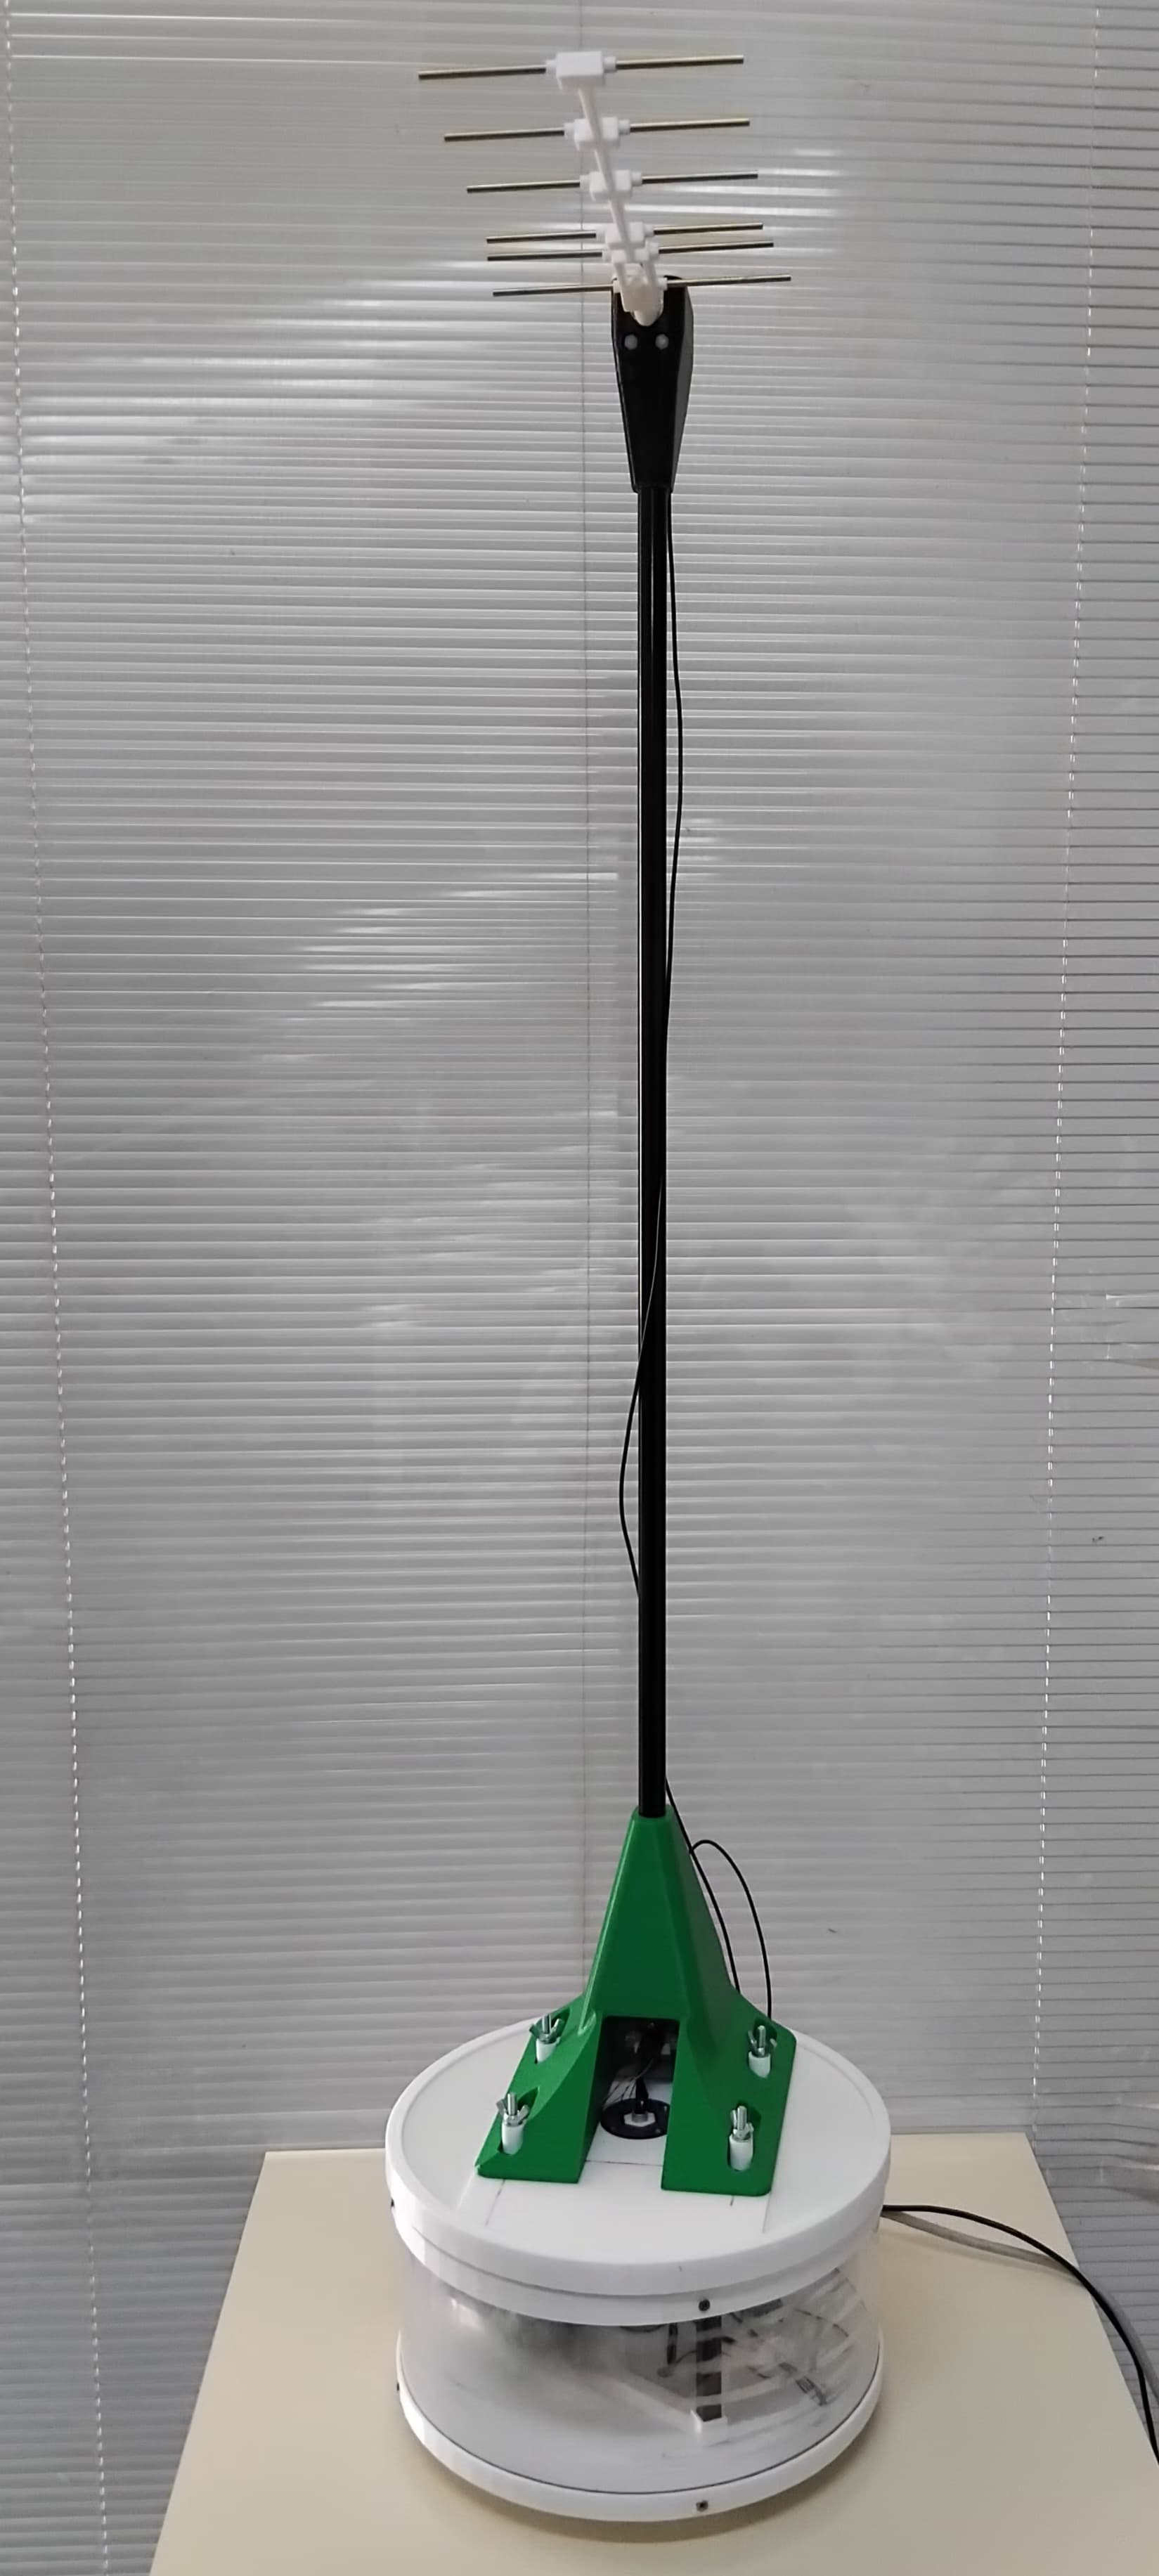
\includegraphics[width=\textwidth]{Imagens/front_view.jpg}
\caption{Front view}
\label{cap1:sec1:fig1:a}
\end{subfigure}
\hspace{3mm}
\begin{subfigure}{0.2555\textwidth}
\centering
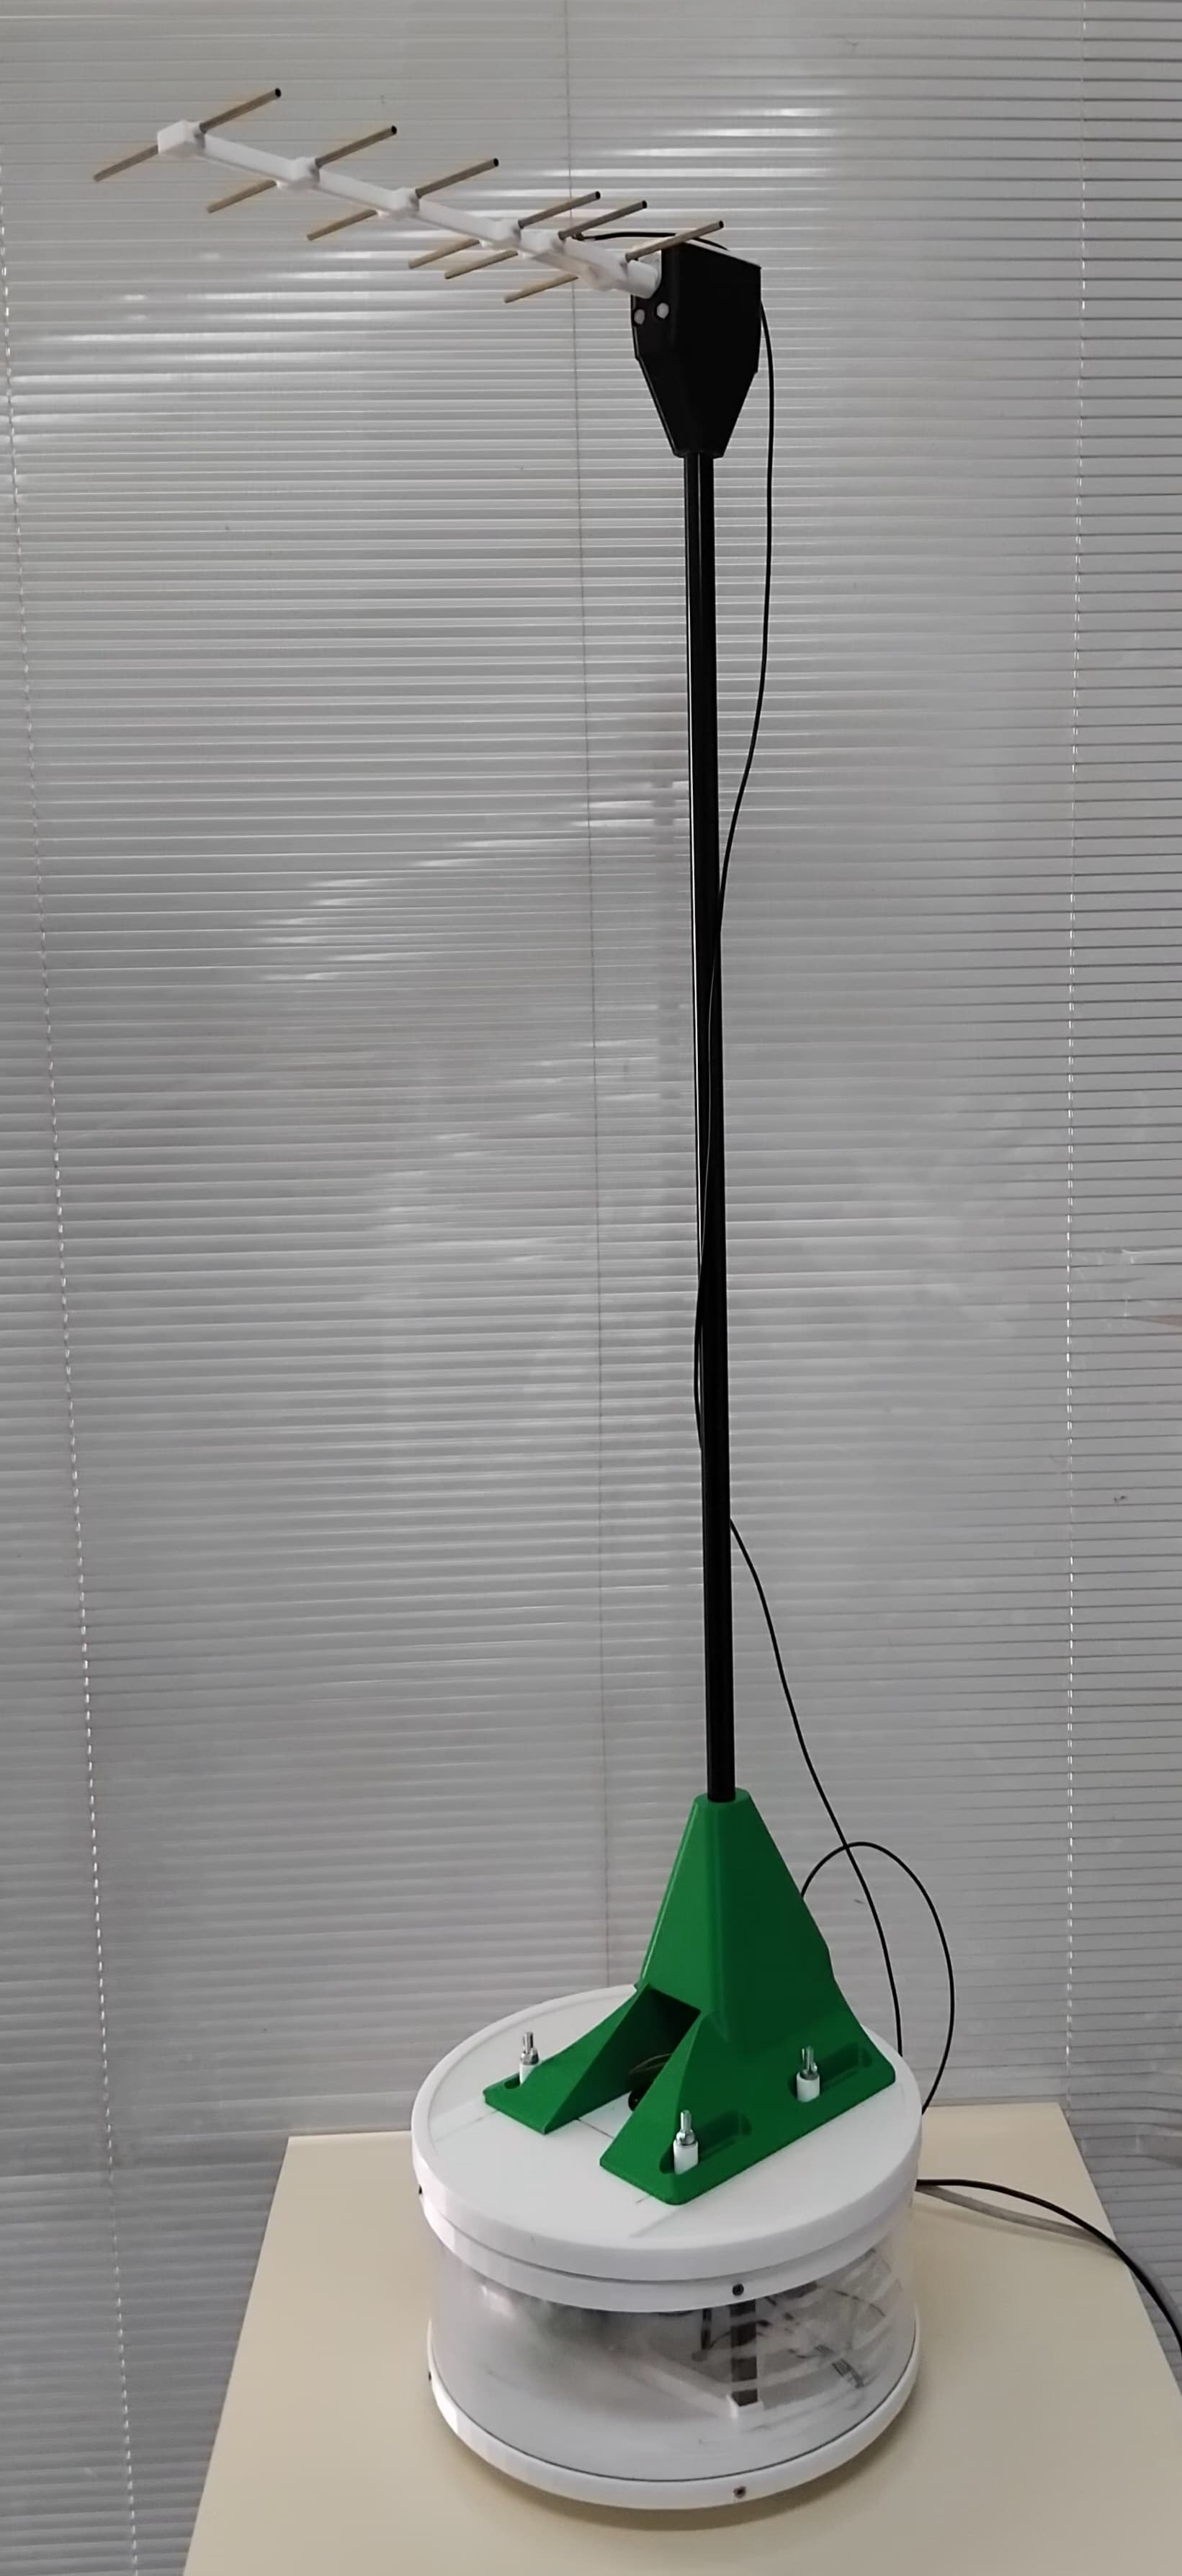
\includegraphics[width=\textwidth]{Imagens/side_view.jpg}
\caption{Side view}
\label{cap1:sec1:fig1:b}
\end{subfigure}
\hspace{3mm}
\begin{subfigure}{0.25\textwidth}
\centering
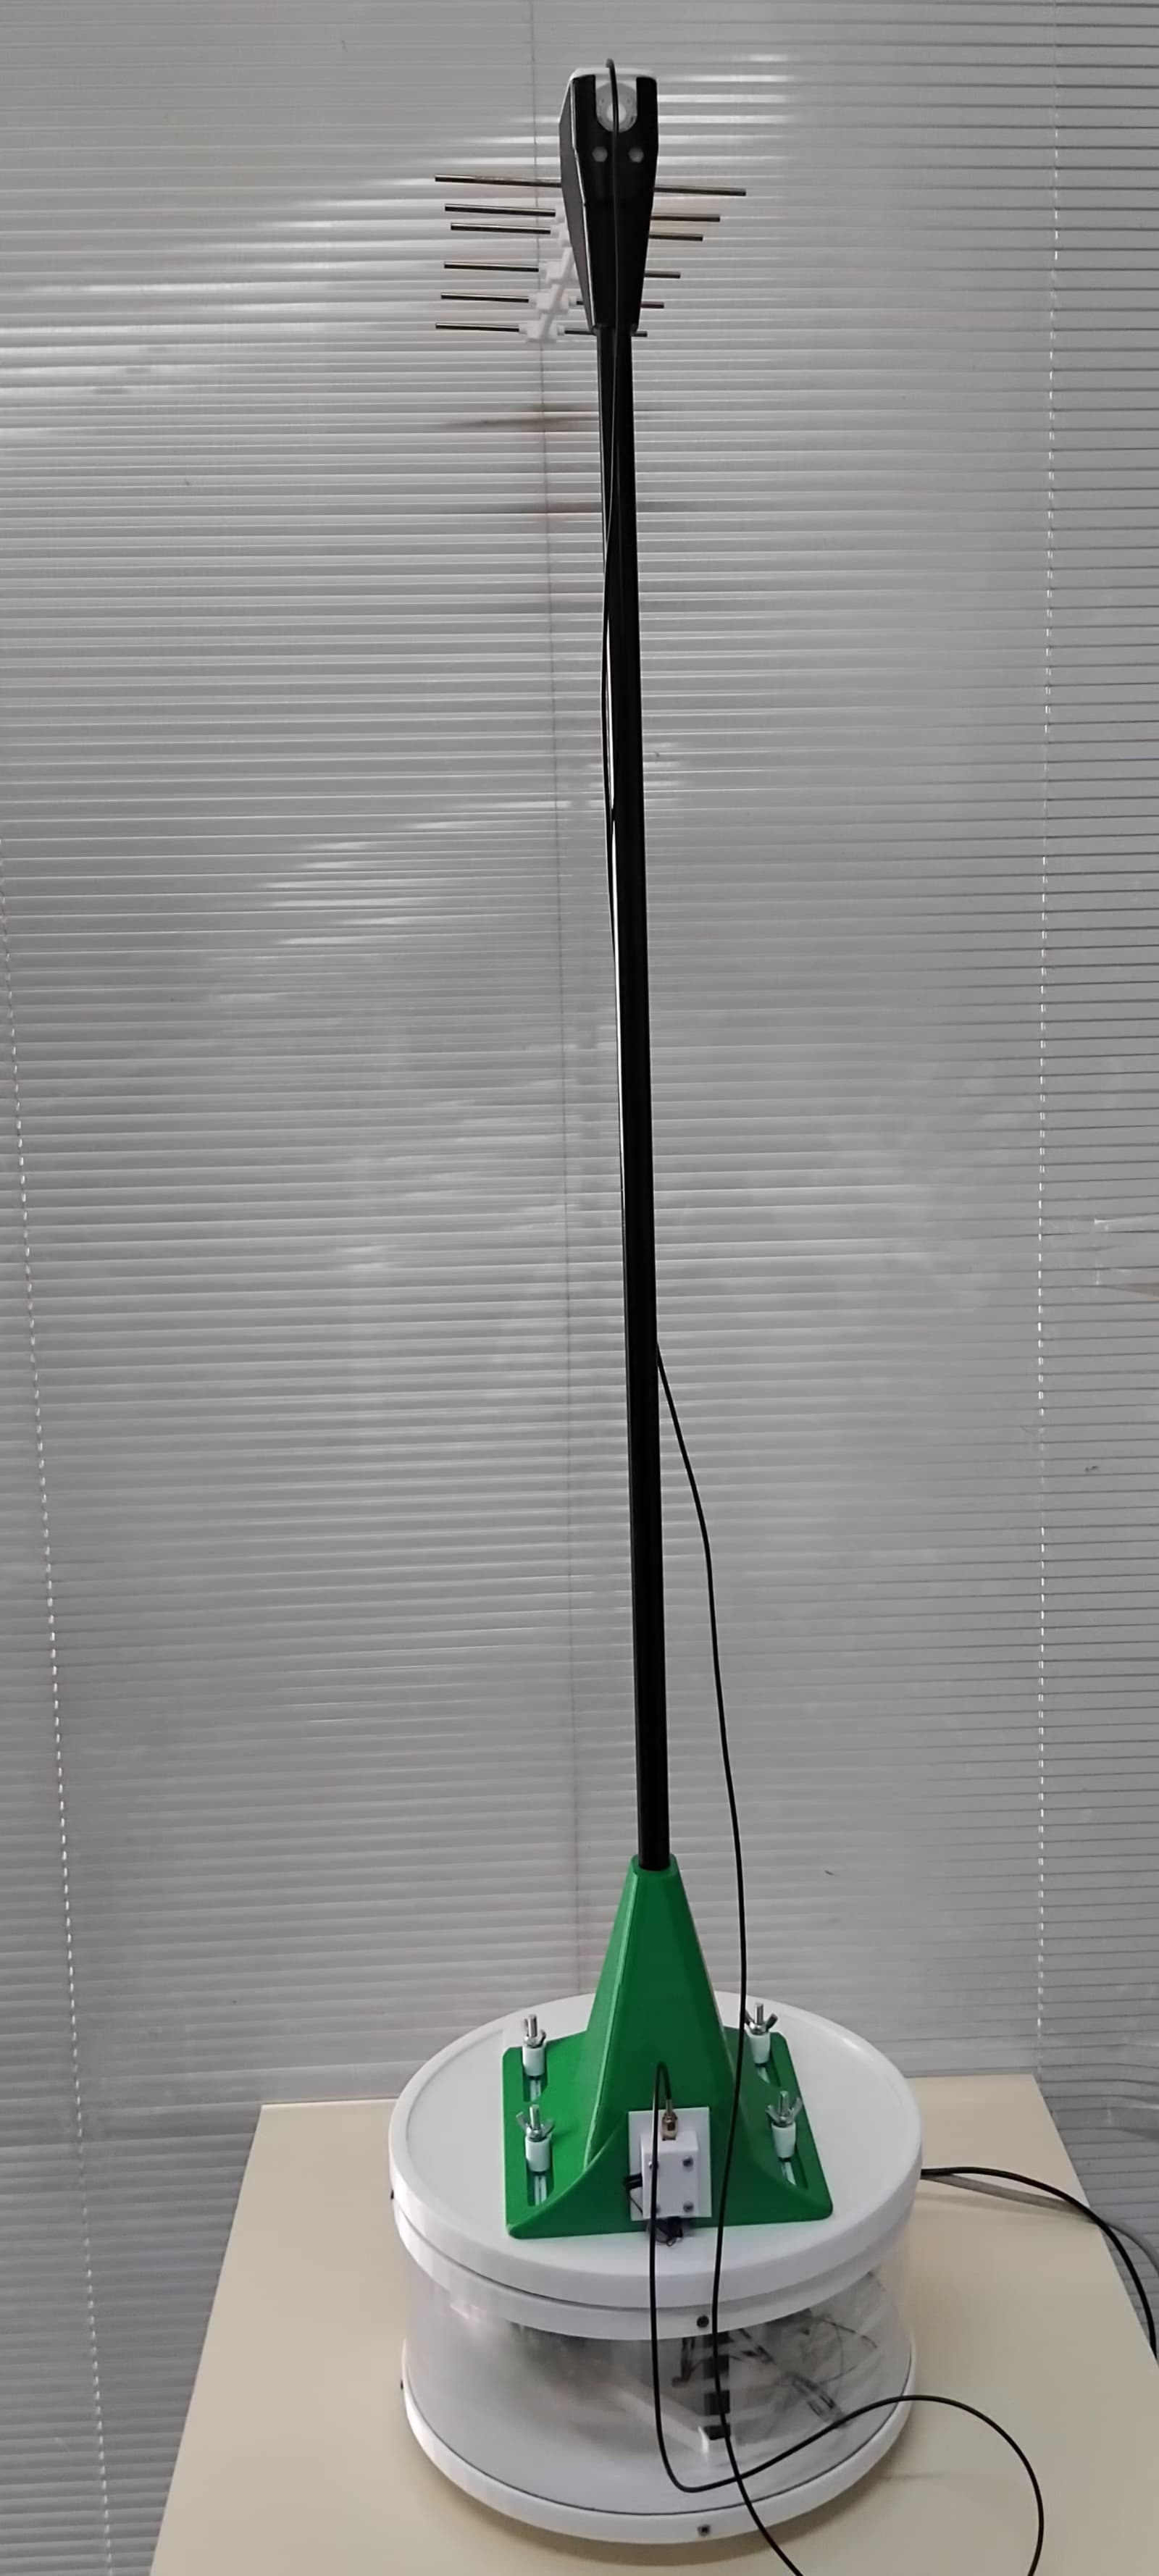
\includegraphics[width=\textwidth]{Imagens/back_view.jpg}
\caption{Back view}
\label{cap1:sec1:fig1:c}
\end{subfigure}
\caption{Overview of the complete antenna radiation pattern measurement system.}
\label{cap1:sec1:fig1}
\end{figure}

%-----------------------------------------------------------------------------------------------------
\section{Objectives}
%-----------------------------------------------------------------------------------------------------

The main objective of this work is to design and implement a low-cost computerised system for measuring antenna radiation patterns, suitable for educational and experimental use. This primary goal emphasises the development of a system that is accessible, reliable, and capable of providing meaningful practical experience in an academic context.

In addition to this, the project also addresses secondary objectives that contribute to the overall functionality and validation of the system. These include the construction of two Yagi–Uda antennas, to transmit and receive signals, the development of a two-axis rotating platform with angular control for antenna positioning, the integration of electronic subsystems for motor control, RF power detection, and data acquisition. Collectively, these secondary objectives support the achievement of the primary goal while ensuring the usability of the system and its educational usefulness.


%-----------------------------------------------------------------------------------------------------
\section{Document Structure}
%-----------------------------------------------------------------------------------------------------

The document is organised into five main chapters, each addressing a specific aspect of the work:

\begin{itemize}
    \item \textbf{Chapter 2 – State of the Art:} Reviews existing commercial antenna measurement systems and related research initiatives, emphasising the need for accessible, low-cost alternatives and setting the context for the proposed system.
    \item \textbf{Chapter 3 – Materials and Methods:} Describes the proposed system in detail, including its mechanical design, electronic subsystems, software development, and validation strategy. The chapter also covers the design and characterisation of the Yagi–Uda antenna, as well as the implementation of impedance matching and balun circuits.
    \item \textbf{Chapter 4 – Results:} Presents the experimental outcomes obtained from the characterisation of individual system components and the complete measurement setup, and compares them with simulated data to evaluate accuracy and repeatability.
    \item \textbf{Chapter 5 – Conclusions and Future Work:} Summarises the main findings, discusses limitations, and suggests ideas for future improvements.
\end{itemize}



%-----------------------------------------------------------------------------------------------------
\section{Scientific Publications}
%-----------------------------------------------------------------------------------------------------

The work developed in this project has also contributed to scientific publication. Two articles have already been produced: one presented at the \textit{5th Symposium of Applied Science for Young Researchers (SASYR)}, and another accepted for presentation at the \textit{13th Technological Ecosystems for Enhancing Multiculturality (TEEM)} conference, the latter being an indexed venue, which reinforces the scientific relevance of the results. 

In addition, the outcomes obtained from the design and validation of the Yagi–Uda antenna provide material for a potential third article, which may be developed in future work.
 
%-----------------------------------------------------------------------------------------------------
\chapter{State of the Art}
\label{cap2:State_Of_The_Art}
%-----------------------------------------------------------------------------------------------------

%-----------------------------------------------------------------------------------------------------
\section{Introduction}
%-----------------------------------------------------------------------------------------------------

Over the last few decades, technology has advanced rapidly, especially in telecommunications. Antennas have a crucial role in this context as they are key elements in the communication chain, upon which the overall performance of the system strongly depends. Since World War I, the design and development of antennas has been a topic of great relevance, initially driven by military applications. Over time, this importance has increased with the introduction of new technologies, such as television, and continues to grow in the current era of mobile communications, including 5G and high-frequency Wi-Fi. The need to characterize and evaluate an antenna's performance has become even more crucial to ensure the efficiency and reliability of communication systems.


To ensure that antennas operate within expected parameters, it is essential to use measurement and calibration systems. These systems allow the evaluation of various antenna characteristics, including radiation pattern, gain, efficiency, and bandwidth. Measuring and validating antenna performance is vital to make sure they meet technical and regulatory specifications.


Radiation pattern measurement is a key step in the design process of antennas and wireless devices. The results of these measurements are used to validate simulated designs and identify potential performance issues before final testing.


While commercially available antenna measurement systems are designed to provide precise and repeatable measurements, they are often expensive. Therefore, custom-made solution are the way when budget is a constraint. These custom-made solutions offer a cost-effective alternative, while addressing specific needs that commercial systems may not cover.

In this chapter, some available commercial solutions for antenna radiation patterns measurement will be first presented. Then, a review is made regarding research and development works that aim to develop similar devices. The goal is to provide a theoretical and practical basis that supports the decision to develop an cost-effective and accurate solution, aligning with the objectives of this project.

%-----------------------------------------------------------------------------------------------------
\section{Commercially Available Products}
\label{cap2:sec2:Commercially Available Products}
%-----------------------------------------------------------------------------------------------------

This section presents commercially available solutions for measuring antenna radiation patterns. These solutions are used in research and development laboratories as well as in companies that need to validate antenna performance across different frequencies. The following descriptions provide a detailed overview of the main features and the purpose for which each system is most suitable. It should be noted that the list presented is not exhaustive and only includes companies that were contacted as part of this study.


\subsection{MegiQ RMS-0460}

According to the supplier, the MegiQ RMS-0460 system, manufactured in the Netherlands, is designed to perform antenna radiation pattern measurements in environments such as laboratories or offices, without requiring an anechoic chamber, as shown in Figure \ref{cap2:sec2:fig1}. It operates over a frequency range of 370 MHz to 6 GHz and supports measurements along three axes. The system offers a measurement accuracy of $\pm 1$ dB and repeatability of $\pm 0.5$ dB. Depending on the configuration, the system can handle loads up to 30 kg. The approximate price is \euro\;16,950.


\begin{figure}[H]
    \centering
    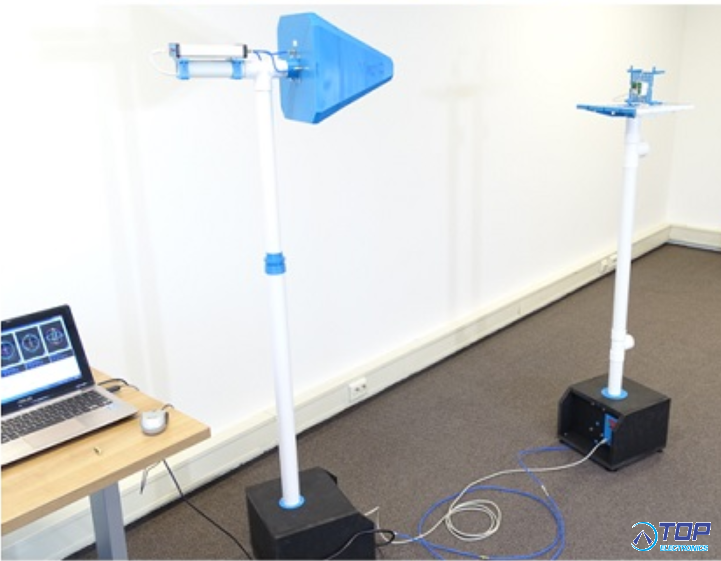
\includegraphics[scale=0.8]{Imagens/MegiQ RMS-0460.png}
    \caption{MegiQ RMS-0460 Measurement System.}
    \label{cap2:sec2:fig1}
    
    \vspace{2mm} % Espaço entre legenda e a fonte
    \small \textit{Source: MegiQ, 2024.} % Fonte da imagem
\end{figure}



\subsection{D6050 Diamond Engineering}

The D6050, produced by Diamond Engineering in the United States, is designed to perform measurements over a frequency range up to 67 GHz, and up to 110 GHz when using waveguides. It offers an angular precision of $0.02^\circ$ and supports loads up to 11.5 kg. The system, depicted in Figure \ref{cap2:sec2:fig2}, features a modular configuration that allows the addition of linear axes for automated measurement. Additionally, it includes software for control and data analysis. The starting price is \euro\;12,880.

\begin{figure}[H]
    \centering
    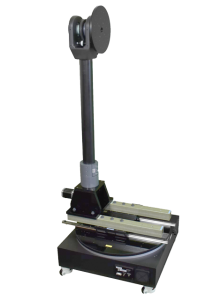
\includegraphics[scale=1.2]{Imagens/D6050.png}
    \caption{D6050 Measurement System.}
    \label{cap2:sec2:fig2}
    
    \vspace{2mm} % Espaço entre legenda e a fonte
    \small \textit{Source: Diamond Engineering, 2024.} % Fonte da imagem
\end{figure}




\subsection{Microwave Factory Co., Ltd. (MWF)}

Microwave Factory Co. Ltd., from Japan, offers an option for measuring antenna radiation patterns, operating in a range from 0.4 GHz up to 300 GHz, depending on the configuration. As shown in Figure \ref{cap2:sec2:fig3}, the system includes an antenna tower, azimuth positioner, elevator, RF absorbers, and control software (MATEOS.NET), enabling 2D radiation pattern measurements and antenna gain analysis. The system is customizable to accommodate equipment with varying weights, with a capacity of up to 1000 kg, which allows it to be used for large-scale projects in controlled environments. It offers an angular precision of $0.03^\circ$ and repeatability of $\pm 0.03^\circ$. However, it requires an anechoic chamber to ensure measurement accuracy. The total price for the complete system is approximately \euro\;368,000.

\begin{figure}[H]
    \centering
    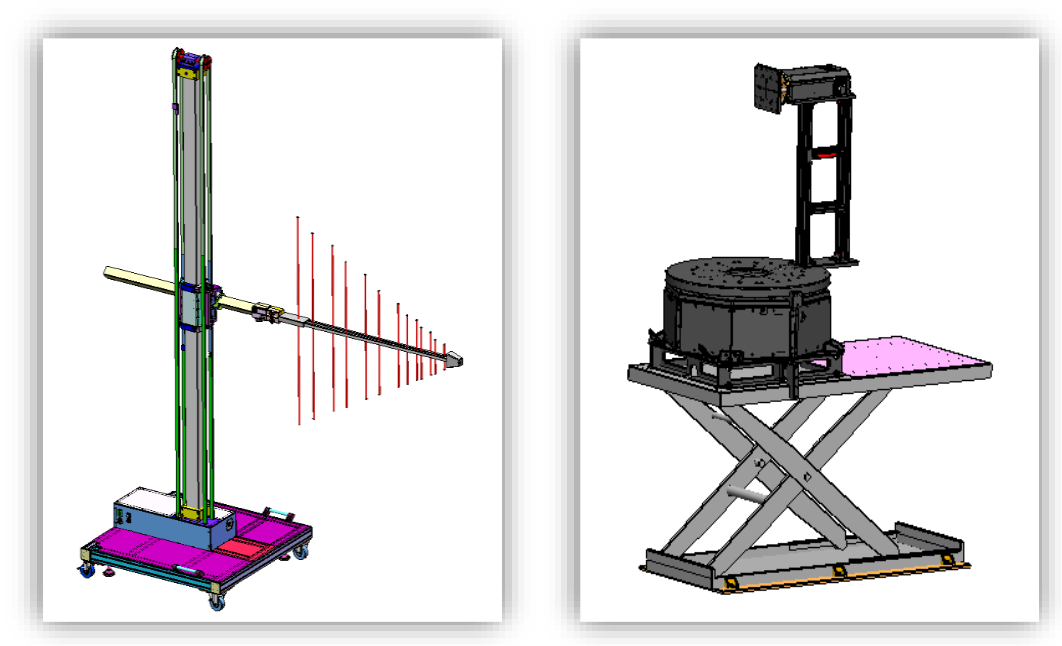
\includegraphics[width=\textwidth]{Imagens/MWF.png}
    \caption{Microwave Factory (MWF) Measurement System representation.}
    \label{cap2:sec2:fig3}
    
    \vspace{2mm} % Espaço entre legenda e a fonte
    \small \textit{Source: Microwave Factory Co. Ltd., 2024.} % Fonte da imagem
\end{figure}


\subsection{S7601A Antenna Measurement System}

The S7601A Antenna Measurement System, developed by Keysight Technologies, a United States company, is also a product for antenna characterization. It operates within a frequency beginning from 10 MHz to 50 GHz and allows for both near-field and far-field measurements. This system supports 2-axis positioning and can handle antennas weighing up to 10 kg. According to the manufacture, it enable measurement accuracy up to $\pm 0.8$ dB, delivering results for various antenna systems, including 5G, satellite, and radar applications. The system includes an integrated anechoic chamber, which, for reference, the price of the S7601A anechoic chamber alone is approximately \euro\;856,000. Additional measurement devices are offered by the same company and can be acquired based on the specific needs of the user. The system is illustrated in Figure \ref{cap2:sec2:fig4}.


\begin{figure}[H]
    \centering
    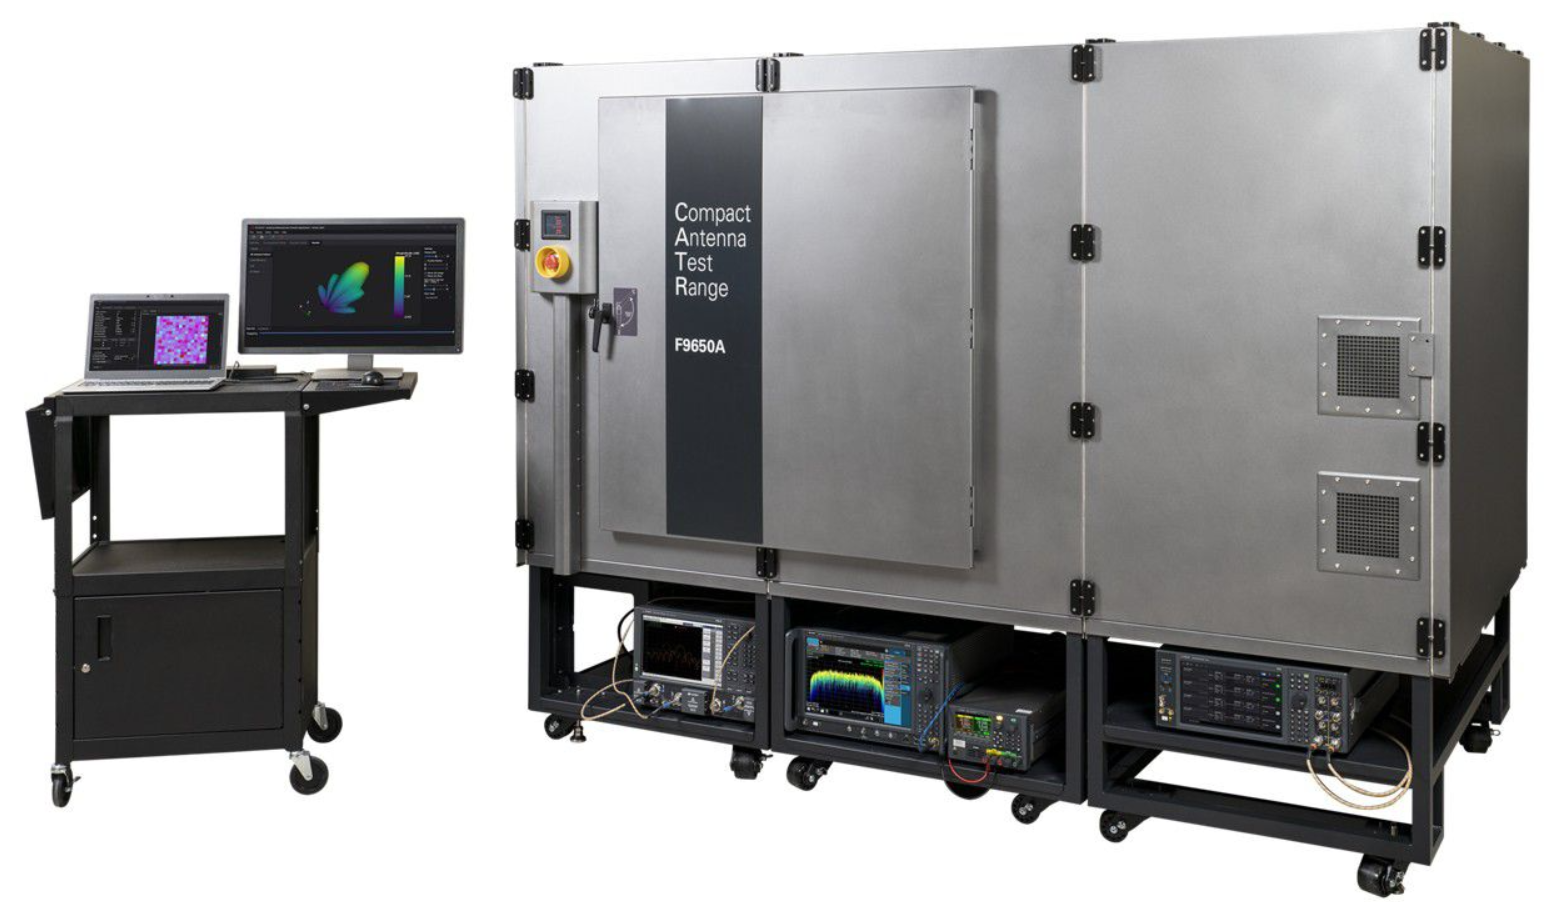
\includegraphics[scale=0.45]{Imagens/S7601A.png}
    \caption{S7601A Antenna Measurement System.}
    \label{cap2:sec2:fig4}
    
    \vspace{2mm} % Espaço entre legenda e a fonte
    \small \textit{Source: Keysight Technologies, 2024.} % Fonte da imagem
\end{figure}


As referred in the beginning of this section, contact was made via email with the companies that manufacture these systems. Despite this, some specific information regarding certain features, such as signal accuracy or load capacity, was either not provided or is not applicable due to possible configurations of the system. This explains the gaps in the comparison provided in Table \ref{cap2:sec2:table1} where data is unavailable or subject to change based on client requirements.

\begin{table}[H]
\centering
\caption{Comparison of Commercial Antenna Measurement Systems}
\resizebox{\textwidth}{!}{%
\begin{tabular}{|l|l|l|l|l|}
\hline
\textbf{Feature}               & \textbf{MegiQ RMS-0460}   & \textbf{D6050 Diamond Eng.} & \textbf{Microwave Factory}   & \textbf{S7601A}             \\ \hline
\textbf{Frequency Range}       & 370 MHz – 6 GHz           & Up to 67 GHz (110 GHz)       & 0.4 GHz – 6 GHz            & 10 MHz – 50 GHz             \\ \hline
\textbf{Measurement Axes}      & 3-axis                    & 2-axis                      & 2-axis                       & 2-axis                      \\ \hline
\textbf{Signal Accuracy (dB)}  & $\pm 1$ dB                     & Not Specified               & Not Specified                & $\pm 0.8$ dB                     \\ \hline
\textbf{Angular Precision ($^\circ$)} & Not specified             & $0.02^\circ$                       & $0.03^\circ$                        & Customizable               \\ \hline
\textbf{Load Capacity}         & Up to 30 kg           & 11.5 kg                     & Up to 1000 kg                & 10 kg                       \\ \hline
\textbf{Environment}           & No chamber required       & No chamber required         & Needs chamber                & Chamber included            \\ \hline
\textbf{Price}                 & \euro\;16,950                   & \euro\;12,880                     & \euro\;368,000                     &  \euro\;856,000 (Chamber only)             \\ \hline
\end{tabular}%
}

\label{cap2:sec2:table1}
\end{table} \vspace{0.15cm}

In conclusion:
\begin{itemize}

\item The MegiQ RMS-0460 system is designed for smaller to medium-sized antennas, with a load capacity of up to 30 kg, depending on the configuration. It operates without requiring an anechoic chamber, making it applicable for environments like laboratories or educational settings, where portability and ease of setup are necessary.

\item The D6050 Diamond Engineering system provides an angular precision of $0.02^\circ$, suitable for applications that require accurate positioning of antennas. It operates within a frequency range up to 110 GHz when using waveguides, and supports high-frequency measurements for medium-sized antennas.

\item The Microwave Factory Co., Ltd. system has the highest load capacity among the compared systems, supporting up to 1000 kg. This makes it the choice for large-scale projects, such as those involving heavy or large antennas. It also provides a frequency range up to 300 GHz, making it suitable for advanced applications in aerospace or defence industries where high precision and anechoic chamber-controlled environments are critical.

\item The S7601A Antenna Measurement System has a load capacity of up to 10 kg and operates within a frequency range of 10 MHz to 50 GHz. It includes an integrated anechoic chamber, allowing measurements without the need for a separate chamber, making it applicable for industries such as telecommunications and satellite testing.

\end{itemize}

The baseline is that any of the solution, even the most cost-effective, is way outside the grasp of many educational institutions. For this reason, do-it-yourself (DIY) solutions provide the most practical approach. In this reference frame, the following section will be devoted to explore academic published researches that describe the development of custom-made antenna radiation pattern measurement rigs.

%-----------------------------------------------------------------------------------------------------
\section{Research and Development Work}
%-----------------------------------------------------------------------------------------------------

Based on the characteristics of the commercial equipment discussed above, it is possible to conclude that, even if they are highly effective and precise, they can also be quite expensive. For many individuals, organizations, and companies, the high costs of these systems may not be justifiable, especially when financial resources are limited.\\
\vspace{0.1em}
\indent As a result, custom-made solutions emerge as an alternative. These solutions allow for the construction of customized measurement systems that can focus on specific antenna characteristics without the need to acquire complete and expensive commercial systems. Additionally, these solutions can be adapted to include functionalities not covered by commercial systems, providing greater flexibility and cost savings.\\
\vspace{0.1em}
\indent \textbf{Research Methodology:} The literature review was conducted using two major academic databases: Google Scholar and IEEE Xplore (Institute of Electrical and Electronics Engineers Xplore). The search aimed to identify existing commercial antenna measurement systems, as well as academic and open-source solutions focusing on low-cost and customisable alternatives. A set of keyword combinations was used to ensure a comprehensive search, including: ``antenna measurement'', ``antenna measurement system'', ``radiation pattern'', ``automated antenna measurement'', ``low-cost antenna measurement'', ``open-source antenna measurement'', ``SDR antenna measurement'', ``Arduino antenna system'', and ``3D-printed antenna measurement''. Boolean operators such as AND were used to refine the queries (e.g., ``antenna measurement'' AND ``radiation pattern''; ``open-source antenna'' AND ``antenna measurement system'').\\
\vspace{0.1em}
\indent Picco and Martin (2011) developed ``An Automated Antenna Measurement System Utilizing Wi-Fi Hardware''. On their work a device was built using commercial Wi-Fi hardware\cite{6157745}. In particular, specifically modified Linksys brand? routers, to measure RF signals at 2.4 GHz. By replacing the original firmware with open-source DD-WRT firmware, they enabled the routers to function as cost-effective tools for measuring the received signal strength indicator (RSSI). Additionally, the system integrates with LabVIEW software to automate the positioning of the antenna under test using stepper motors. Although the system operates in a non-anechoic environment, the published results suggest that inaccuracies are kept controlled while providing a viable low-cost solution for educational and research settings.

In Junfithrana \textit{et al.} (2017), ``Development of Automated Antenna Radiation Pattern Measurement Using Rotator Application Model to Increase Accuracy'', the authors proposed an automated system that uses a two-axis rotator model controlled by microcontrollers\cite{8308101}. This setup is integrated with a vector network analyzer and the control software was developed in LabVIEW. The work highlights how the use of accessible components can increase measurement accuracy, making the system a practical and economical alternative to commercial solutions.

Simanjuntak \textit{ et al.} (2019), presents the ``Preliminary Design of Automatic Antenna Radiation Pattern Measurement System for Antenna and Propagation Laboratory Course'', in which the authors develop an automated radiation pattern measurement system using microcontrollers\cite{Simanjuntak2019/02}. This study demonstrates that an accessible and portable system can be implemented to be used in educational environments, providing quick and accurate measurements without the need for expensive commercial equipment.


All the above papers exemplify how custom solutions can be adapted to meet specific needs, offering an efficient alternative to commercial systems. They offer a solid foundation for developing new approaches that combine cost-effectiveness, flexibility, and innovation, which is aligned with the goal of this project.


Within the maker community, open-source solutions have gained prominence in the field of antenna measurement due to their flexibility, cost-effectiveness, and adaptability to different research and educational contexts. Examples of such approaches include the work developed by Weber State University, which proposed an antenna pattern measurement system using open-source components, such as Software-Defined Radios (SDRs), Arduino microcontrollers, and GNU Radio software. These studies present the continuous evolution and improvement of accessible and highly effective antenna measurement systems.


Also, in ``Open-Source Antenna Pattern Measurement Validation Using FEKO'' (2020) an antenna pattern measurement system developed using SDRs and 3D-printed hardware, is presented\cite{9196138}. The system validation was conducted by comparing experimental measurements of antenna radiation patterns with theoretical simulations generated by the FEKO simulation software. The results demonstrated that the low-cost system could replicate measurements with a high degree of accuracy, making it an ideal tool for undergraduate-level investigations on antenna theory and practical measurements.


In the same year, ``Open-Source Antenna Pattern Measurement System'' (2020) presents the development of a measurement system by replacing Wi-Fi routers with SDRs to expand the frequency range (30 MHz to 6 GHz) over which measurements can be performed\cite{9280870}. This enhanced version of the system addresses challenges related to position control and measurement accuracy, using stepper motors controlled by an Arduino with open-source GRBL firmware. The study highlights how the replacement of components and the integration of new control and signal processing methods helped improve the system's precision and versatility while keeping it accessible and suitable for educational environments.


Finally, the most recent work among the studies reviewed, "Open-Source Antenna Pattern Measurement System: SDR-based Student Research and Development" (2022)\cite{finger2022open}, presents the latest updates to the system, including significant hardware and software improvements. Hardware upgrades include replacing Polyvinyl Chloride (PVC) components with Computer-Aided Design (CAD)-modelled and 3D-printed parts, increasing the system's mobility and adaptability for use in multiple noisy environments. The software was enhanced with new versions of Python, GNU Radio, and Linux, and advanced noise mitigation techniques and modulation control were incorporated to further improve measurement accuracy. The article highlights the system's success as a robust and flexible educational tool, creating opportunities for collaborative research and project development among electrical engineering students.


%-----------------------------------------------------------------------------------------------------
\chapter{Materials and Methods}
\label{chap:materials_methods}
%-----------------------------------------------------------------------------------------------------


Following the review of commercial systems and research initiatives discussed previously, this chapter presents the practical implementation of a low-cost antenna radiation pattern measurement system. Designed to meet educational and experimental needs around the 868 MHz ISM band, the proposed setup combines mechanical design, custom electronics, and software integration. This chapter describes the materials used, the configuration of each subsystem, and the validation methodology. Additionally, it highlights RF-related improvements, including a custom-designed air-core choke balun and an impedance matching network.
\vspace{0.1em}

%-----------------------------------------------------------------------------------------------------
\section{Proposed System Description}
\label{sec:system_description}
%-----------------------------------------------------------------------------------------------------

The antenna radiation pattern measurement system was developed with an emphasis on low cost, modularity, and suitability for educational and experimental applications. Built using commercially available components and custom-fabricated parts, the system allows for easy replication and future enhancements. It is composed of the following main subsystems:

\begin{itemize}
    \item \textbf{Mechanical substructure} with two independent rotational axes (azimuth and perpendicular) for the receiving antenna.
    \item \textbf{Electronic control system} based on the ATmega328P microcontroller (Arduino Uno).
    \item \textbf{RF power measurement circuit} using the AD8313 logarithmic detector.
    \item \textbf{MATLAB software suite} for motor control, data acquisition, and real-time visualization.
\end{itemize}

\subsection{System Architecture}
\label{subsec:system_architecture}

The system includes two rotational axes: the azimuth axis, located at the base, and a perpendicular axis at the top, which enables angular scanning in an orthogonal plane. Depending on the antenna mounting orientation, this perpendicular axis can be adapted to perform elevation, as shown in Figure \ref{cap3:sec1:fig1}. Both axes are actuated by NEMA 17 stepper motors with $1.8^\circ$ step angle, driving belt-and-pulley mechanisms. To prevent twisting of the coaxial cable and transmission wires, the motor moves up to $180^\circ$ in one direction, returns to the home position, and then moves up to $180^\circ$ in the opposite direction.

\begin{figure}[H]
    \centering
    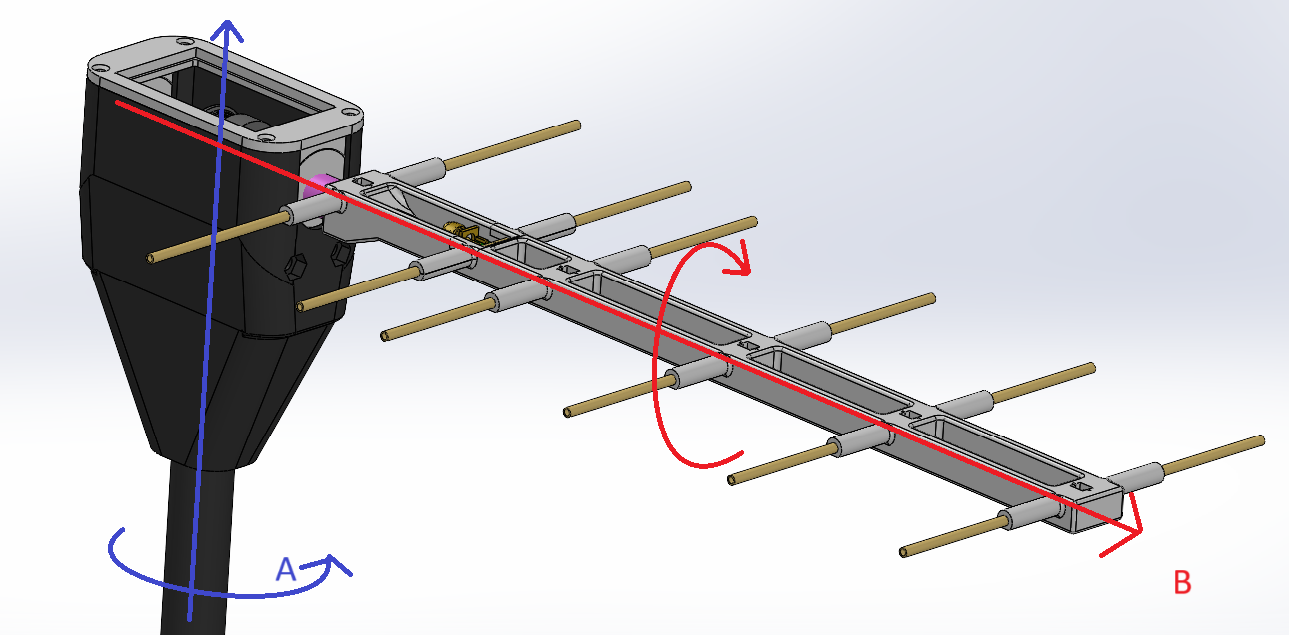
\includegraphics[width=0.85\textwidth]{Imagens/antenna_rotation.png}
    \caption{CAD model of the rotating platform with two degrees of freedom. Axis ``A'' corresponds to the azimuth rotation and axis ``B'' to the perpendicular rotation, which can be configured as the elevation axis.}
    \label{cap3:sec1:fig1}
\end{figure}

The mechanical transmission system, based on belts and polies, was specifically designed to achieve a resolution of approximately $1 ^ \circ$ of revolution per motor step. This was achieved by using custom-designed gears with a 1.8:1 ratio. The rotating assembly is supported by low-friction components to ensure smooth motion and reproducibility of measurements.

It is worth noting that despite the mobile platform responsible for rotating the antenna under test, the complete system also includes a fixed structure that acts as a transmitting station. This fixed base has dimensions and construction characteristics similar to the rotational platform, such as mounting height and accommodation of the transmitting antenna. Even without motorised degrees of freedom, the antenna installed on this base can be manually oriented on different axes, allowing for various configurations, such as azimuth or orthogonal alignment, according to the desired experiment. Thus, the assembly consists of two complementary mechanisms, assisting in the measurement of radiation patterns in different scenarios.


\subsection{Components Used}
\label{subsec:components_used}

The main components used in the construction of the system are:

\begin{itemize}
 \item \textbf{Stepper Motors}: NEMA 17 bipolar stepper motors with $1.8 ^ \circ$ per step, configured for 1/16 microstepping using DRV8825 drivers. These motors were selected over commun low-cost servo motors due to their superior precision and high torque, which are crucial for achieving accurate angular positioning required for antenna pattern measurements. 
\item \textbf{Microcontroller}: Arduino Uno board, based on the ATmega328P, is responsible for coordinating motor motion, executing homing routines, and reading sensor data. The Arduino Uno was chosen for its ease of programming, widespread community support, and cost-effectiveness, making it an ideal platform for an educational and experimental system.
 \item \textbf{RF Power Sensor}: Analog Devices AD8313 module, operating from 100~MHz to 2.5~GHz range, with a dynamic range of up to 70~dB. This sensor was selected because it can be supplied inexpensively from the Asian market. %due to its wide operating frequency range and high dynamic range, which are essential for accurately measuring varying RF power levels across the target ISM band of 868 MHz.
\item \textbf{Magnetic Position Sensors}: Hall-effect magnetic sensors (KY-035 49E), used for homing reference detection on each rotational axis. These sensors provide a reliable and low-cost solution for precise homing, ensuring consistent starting positions.
\item \textbf{Power Supply}: Industrial 12~V DC, 2~A power supply (Orno OR-ZL-1631), rated at 24~W with IP20 protection and 230~V Alternating Current (AC) input, providing regulated voltage to all system components. A standard power supply was chosen for its reliability and capability to provide stable and sufficient power to all active components of the system.
\item \textbf{Mechanical Structure}: The platform consists of a one-meter fibreglass tube (non-conductive and lightweight), 3D-printed pulleys and brackets, and a wooden base in circular shape. Non-metallic materials were deliberately selected near the antenna to avoid reflections or distortions by the radiation pattern. Even the internal bearings are from nylon materials. Some components of the mechanical structure, such as the wooden base, were sourced in a manner that did not significantly impact the final cost of the project, further aligning with the low-cost objective. Fibreglass and Polylactic Acid (PLA) were chosen for their non-conductive, lightweight properties, minimizing interference and ensuring the structural integrity of the rotating assembly without affecting RF measurements.
\item \textbf{RF Generator}: It is a handheld RF signal generator which is used as a signal source. It operates in a frequency range from 100 kHz up to 6 GHz, offering both CW (Continuous Wave) and sweep modes, with output power from approximately –60 dBm to +15 dBm. Detailed characterisation of both the signal generator and the antenna systems in transmitter and receiver configurations will be present later.

\end{itemize}

% \subsection{Transmitter}

% It is important to mention that, although a commercial RF source was employed, the transmitting antenna and its support structure are functionally identical to the receiving system. The transmitter is a fixed installation, and has the same non-conductive fibreglass tube support, PLA antenna mount, and wooden base as the receiver.

% A handheld RF Explorer Signal Generator was used as the signal source. The device operates in a frequency range from 100 kHz up to 6 GHz, offering both CW and sweep modes, with output power from approximately –40 dBm to +10 dBm. Detailed characterisation of both the signal generator and the antenna systems in transmitter and receiver configurations will be present later.

%-----------------------------------------------------------------------------------------------------
\section{Electrical Subsystem}
\label{subsec:electrical_subsystem}
%-----------------------------------------------------------------------------------------------------



As illustrated in the block diagram in Figure~\ref{cap3:sec2:fig1:a}, the electrical control system is based on an Arduino Uno board (ATmega328P), combined with a dual stepper motor driver shield. This shield integrates two DRV8825 drivers, each configured for 1/16 microstepping via onboard Dual In-line Package (DIP) switches. It simplifies the electrical connections and consolidates the power and control interfaces for the stepper motors.
\begingroup
\setlength{\textfloatsep}{2pt}
\setlength{\intextsep}{2pt}
\begin{figure}[H]
    \captionsetup{aboveskip=1pt,belowskip=1pt}
     \centering
     \begin{subfigure}{0.48\textwidth}
         \centering
         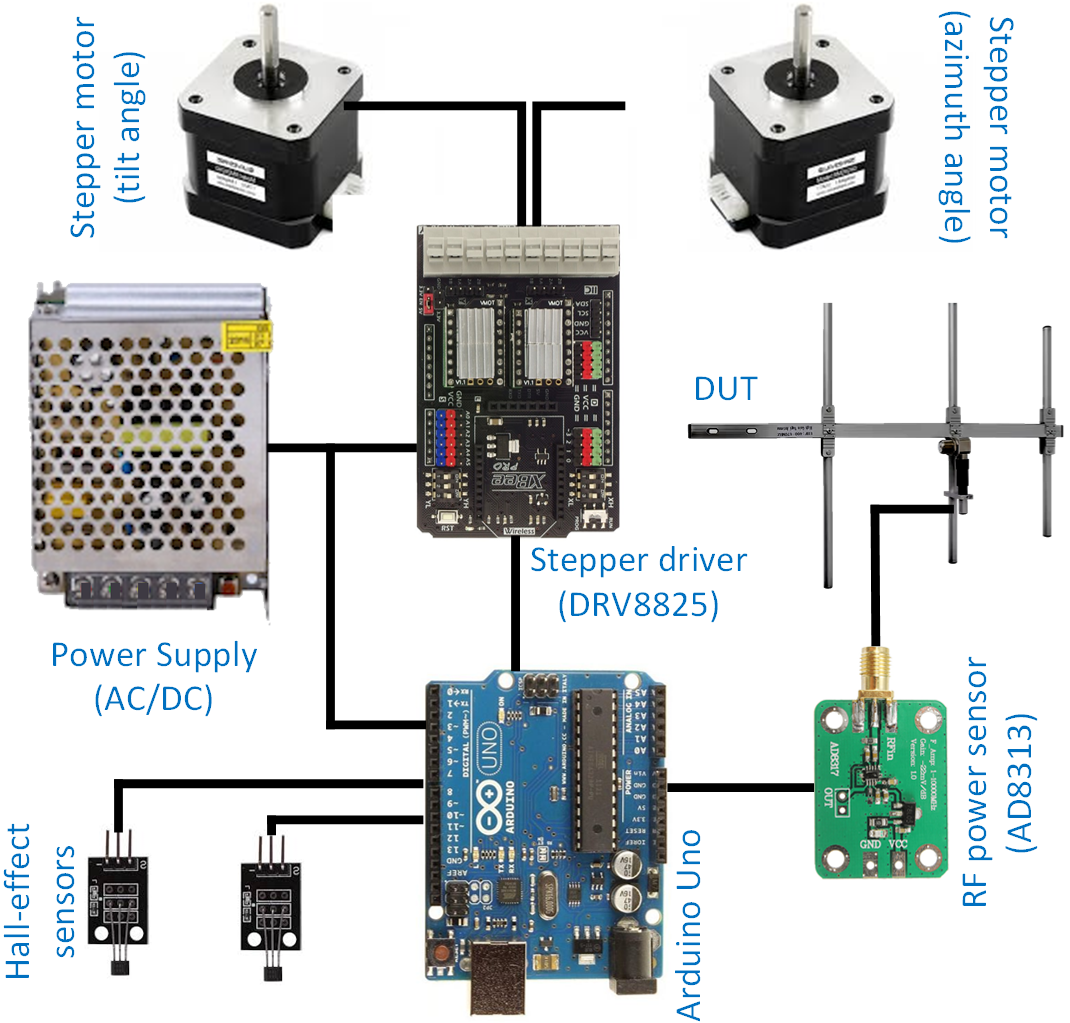
\includegraphics[width=\textwidth]{Imagens/hardware_block_diagram_v2.png}
         \caption{Block diagram of the electrical system}
         \label{cap3:sec2:fig1:a}
     \end{subfigure}
     \hspace{1mm}
     \begin{subfigure}{0.48\textwidth}
         \centering
         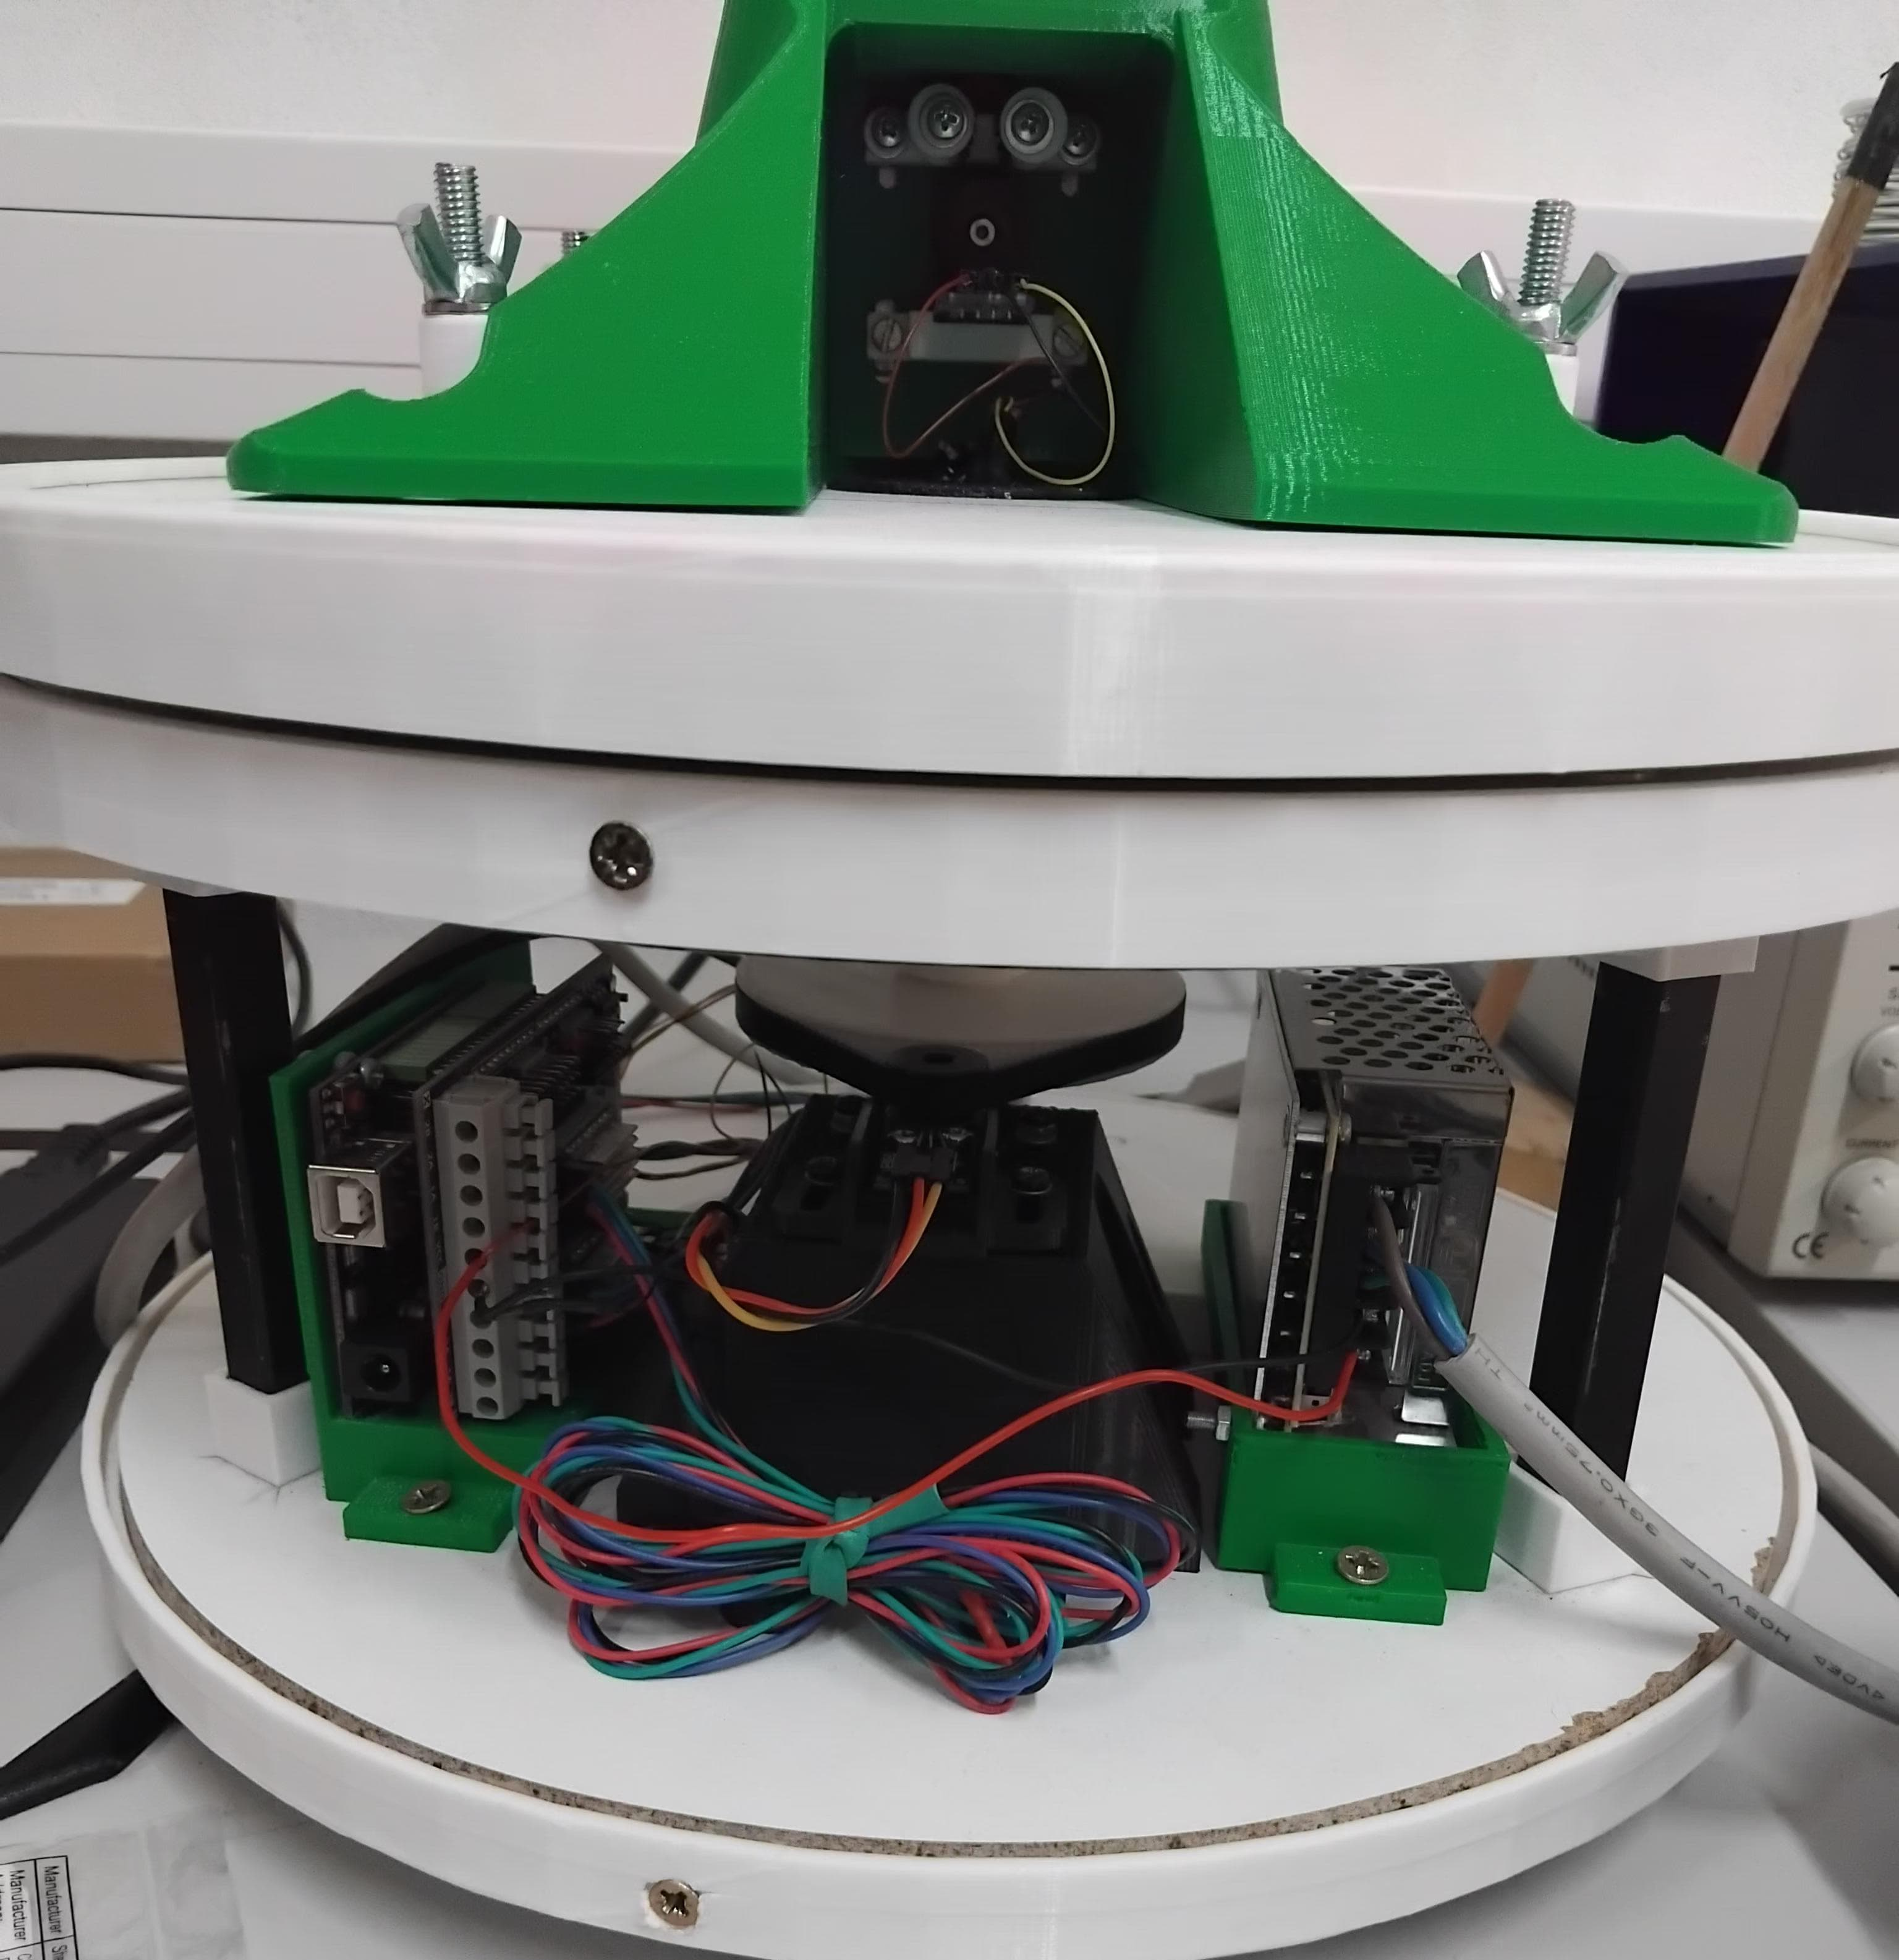
\includegraphics[width=\textwidth]{Imagens/system_real_photo.jpg}
         \caption{Assembled base of the measurement system}
         \label{cap3:sec2:fig1:b}
     \end{subfigure}
        \caption{Block diagram and photo of the electrical system, including key components like the Arduino Uno, DRV8825 driver shield, power supply, sensors, RF detector (AD8313), Device Under Test (DUT), stepper motors, and internal wiring.}
        \label{cap3:sec2:fig1}
\end{figure}
\endgroup
\vspace{-0.1em}

The H-bridge shield receives 12~V from the external power supply, which is then distributes power to the stepper motors and Arduino board. It also powers auxiliary components, such as the Hall-effect sensors and the RF power detector module. The AD8313 module, crucial for the measurement process, converts the incoming RF signal (from 0.1 to 2.5 GHz, with an input impedance of $50~\Omega$) into a DC voltage output, typically ranging from 0.5~V to 1.65~V. Its detection slope is approximately 18~mV/dBm, allowing the conversion of RF power to a measurable voltage signal for the microcontroller. The onboard voltage regulation supports both 5~V and 12~V levels as required by each module.

\indent Each of the two rotational axes includes a Hall-effect sensor positioned to detect a small magnet mounted on the corresponding gear. These sensors are used to perform an automated homing procedure during system initialisation. A dedicated routine implemented in the firmware enables the system to identify the reference position (zero-degree point) of both axes. This ensures reliable absolute positioning throughout the measurement process, compensating for the lack of closed-loop feedback in typical stepper motor systems.\\
\vspace{0.1em}
\indent The wiring of the system is organised and modular, as illustrated by the assembled base in Figure~\ref{cap3:sec2:fig1:b}, and is facilitated by screwless terminals in the shield and the clear allocation of digital I/O (Input/Output)  pins (D4 to D8 and D12) for motor control. The shield also offers expansion capabilities, including $I^2C$ (Inter-Integrated Circuit) headers and XBee-compatible sockets, although wireless features were not used in the present implementation.

%-----------------------------------------------------------------------------------------------------
\section{Assembly}
\label{sec:electrical_wiring_assembly}
%-----------------------------------------------------------------------------------------------------

This section details the specific electrical interconnections and physical assembly of the system's components, providing understanding of the wiring implementation. The complete electrical schematic, illustrating all pin-level connections, is presented in Figure~\ref{cap3:sec3:fig1}.

The central control unit, an Arduino Uno board, interfaces with the various modules of the system primarily through a dedicated Dual Bipolar Stepper Motor Shield. This shield occupies all available pins on the Arduino, simplifying the overall wiring by consolidating power and control interfaces. The shield includes dedicated slots for the two DRV8825 stepper motor drivers (D1 and D2), which control the azimuth and perpendicular axes.

The stepper motors (M1 and M2) are connected to the DRV8825 drivers via specific terminals in the shield. For both motors, the wiring follows a standard bipolar configuration, with coil wires from 1 to 4 connected to pins 2B, 2A, 1B, and 1A on their respective DRV8825 drivers.

\begingroup
\setlength{\textfloatsep}{4pt}
\setlength{\intextsep}{4pt}
\begin{figure}[H]
    \captionsetup{aboveskip=2pt,belowskip=2pt}
    \centering
    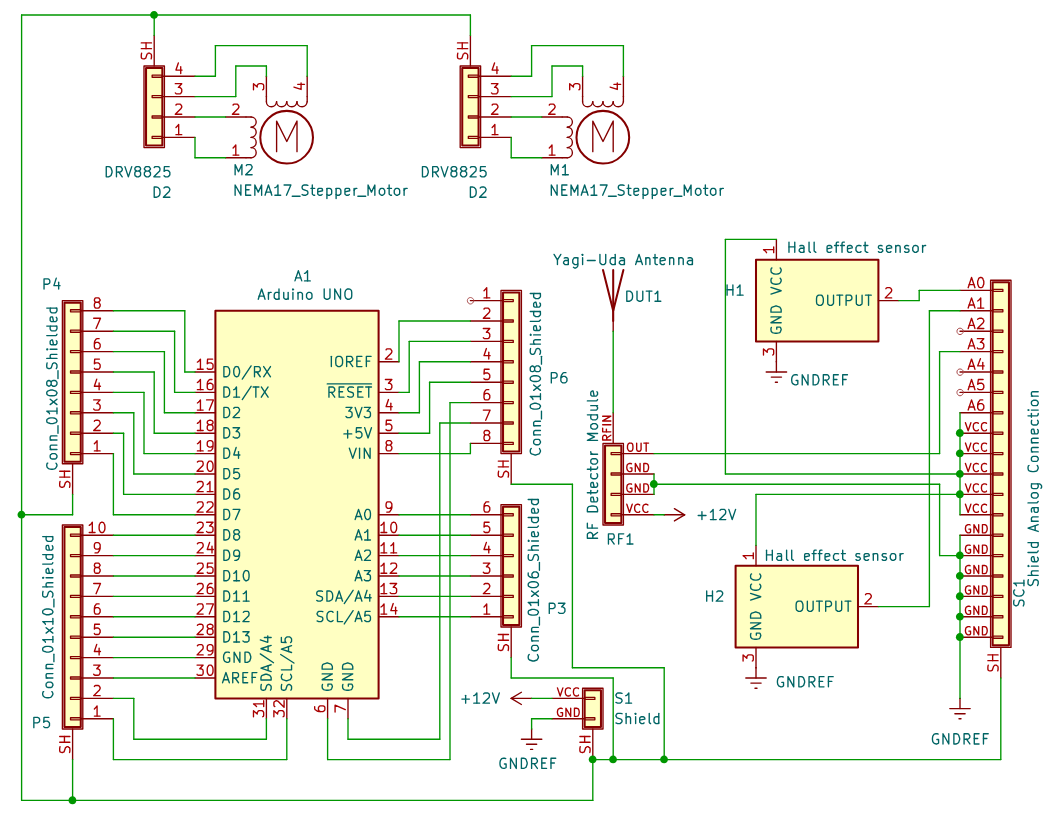
\includegraphics[width=0.7\textwidth]{Imagens/esquematico_ligacao.png}
    \caption{Detailed electrical schematic of the measurement system, illustrating component interconnections and pin assignments.}
    \label{cap3:sec3:fig1}
\end{figure}
\endgroup

\vspace{-0.1\baselineskip}

\indent Auxiliary components, such as the Hall-effect magnetic position sensors and the RF power detector module, connect to specific analog input pins provided by the shield. Sensor 1 is connected to analog pin A0, and Sensor 2 to analog pin A1. The AD8313 RF power module's analog output is connected to analog pin A3 of the shield, allowing the Arduino Uno to read the converted RF power signal.\\
\vspace{0.1cm}
Power distribution is managed centrally by the shield. An external 12V DC power supply provides the primary input to the shield. From this input, the shield directly supplies 12~V to both the stepper motors (via the DRV8825 drivers) and the AD8313 RF power module. Additionally, the shield incorporates an onboard voltage regulator that steps down the 12~V input to provide a stable 5~V supply, which powers the Arduino Uno board itself and the Hall-effect sensors. This integrated power management simplifies the wiring and ensures proper voltage levels for all components.\\
\vspace{0.1cm}
The shield also provides 5~V or 12~V output, depending on the physical configuration. In addition to the analog pins, the shield has digital pins, which were not used in this project but may be decisive in different approaches.



%-----------------------------------------------------------------------------------------------------
\section{Software Development}
\label{sec:software_development}
%-----------------------------------------------------------------------------------------------------
The software for the antenna radiation pattern measurement system comprises two main modules: Firmware implemented on an Arduino board, for motor control and a data acquisition and visualisation module developed in MATLAB.

The MATLAB and Arduino interact through the UART (Universal Asynchronous Receiver-Transmitter) protocol, following a sequence that begins with MATLAB, which initiates the measurement process by sending the scan parameters such as angular resolution and rotation range. The Arduino then executes the commands, moving the stepper motors through their drivers, performing the homing function with the Hall-effect sensors, and coordinating the acquisition of RF power values from the detector module. As the platform rotates stage by stage, the Arduino collects the corresponding measurements and transmits them back to MATLAB. In the meantime, MATLAB stores the data in a matrix, and after all measurements, the radiation pattern is plotted. This command $\rightarrow$ execution $\rightarrow$ response loop gives synchronisation between mechanical actuation and signal acquisition, helping in the measurement results.

The Arduino module controls the stepper motors, also performing a homing procedure to align the antenna to a $0 ^ \circ$ reference point. This reference detection is achieved by Hall-effect sensors. Rotations is carried out in increments (e.g., $1 ^ \circ$) according to commands received from MATLAB. Status confirmations are sent back via UART to ensure synchronisation. 

The MATLAB script communicates with the Arduino via a virtual communication (COM) port, employing the built-in \textit{serialport()} interface of MATLAB. The MATLAB function acquires RF signal data from the RF Module and stores it in a data matrix. It processes parameters such as directivity and generates polar plots (2D/3D) to visualise the antenna radiation pattern. 

The UART communication, established over a USB (Universal Serial Bus) connection, follows a command-response pattern, with MATLAB acting as the master and the Arduino as the slave. MATLAB sends rotation commands, and the Arduino returns measured power data in dBm. The data flow, illustrated in Figure~\ref{cap3:sec4:fig1}, begins with configuration in MATLAB, followed by command transmission, platform rotation, signal measurement, data storage, processing, and visualisation. 




\begin{figure}[H]
    \centering
    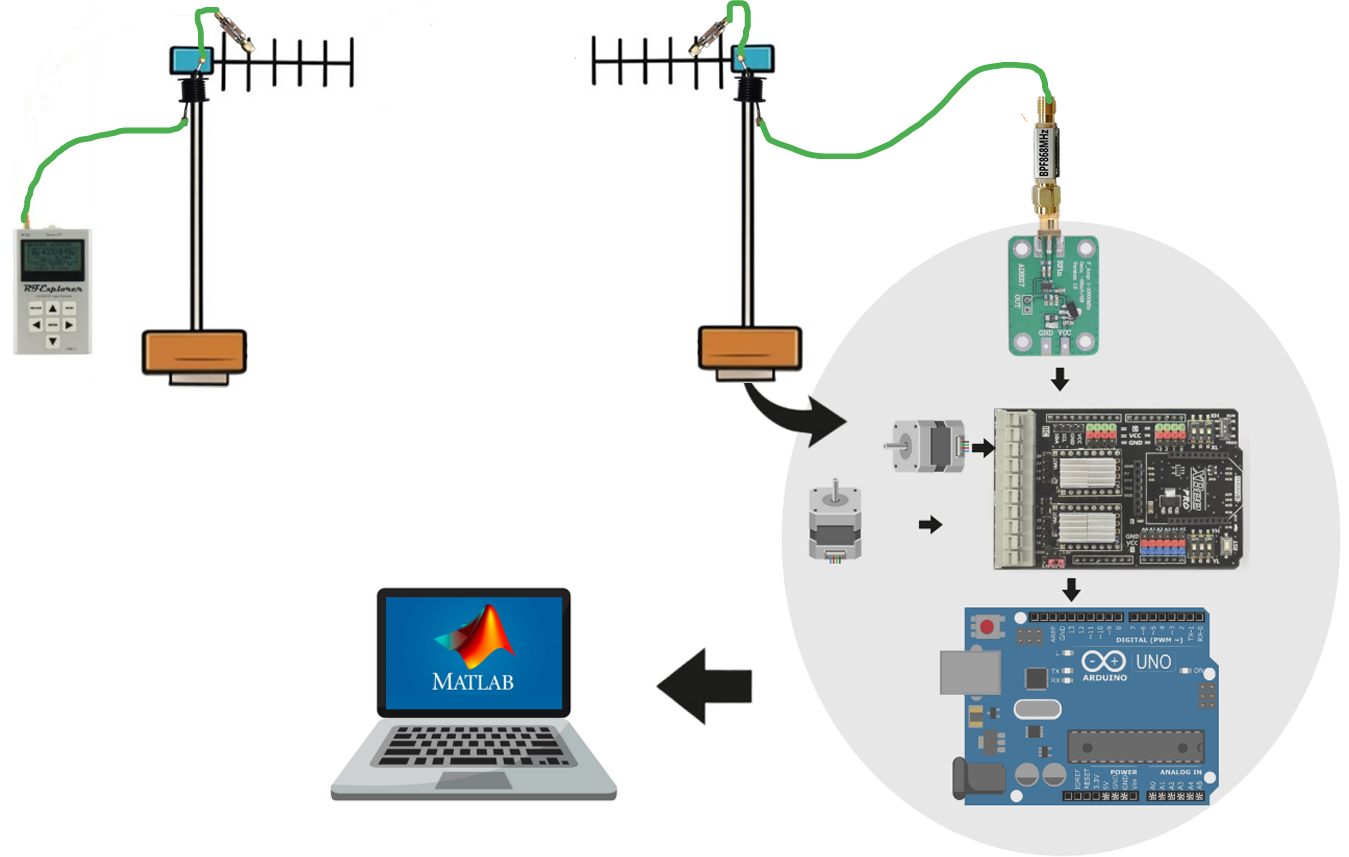
\includegraphics[width=0.9\textwidth]{Imagens/hardware_schematic.png}
    \caption{Schematic showing the flow of the signal from generation to analysis.}
    \label{cap3:sec4:fig1}
\end{figure}



%-----------------------------------------------------------------------------------------------------
\section{Validation Strategy}
\label{sec:validation_strategy}
%-----------------------------------------------------------------------------------------------------

To confirm the accuracy and reliability of the system, a series of validation tests were conducted following a structured testing protocol. This protocol began with characterisation of the transmitting and receiving antennas, as well as the bandpass filter, using a nanoVNA at 868 MHz in the ISM band. The filter, centred at 868 MHz with a bandwidth of 10 MHz, was selected for its ability to mitigate noise, though it introduced approximately 3 dB insertion loss attenuation. A linear model for signal power conversion was derived from the characterisation of the module, aligning closely with the datasheet specifications of the manufacturer.

The measurements were performed in an open environment to minimise unwanted reflections, as indoor settings would introduce excessive interference. In an ideal scenario, tests would be carried out in vacuum or an anechoic chamber, but, due to practical constraints, an outdoor setup was employed with consistent conditions across all trials. The radiation pattern was measured across azimuth angles ($0 ^ \circ$ to $360 ^ \circ$, $5 ^ \circ$ resolution), with 100 samples were averaged at each angle to reduce noise. To minimise cumulative angular errors and prevent cable entanglement (as wires were routed through tubes), measurements were performed bidirectionally: the platform rotated $180 ^ \circ$ in one direction, returned to the initial position, and then rotated $180 ^ \circ$ in the opposite direction. Ten measurement cycles were carried out to assess repeatability, with the averages plotted to verify consistency. The experimental results were compared with CST Studio Suite\footnote{The free educational version of this software was used in the simulations.} simulations, showing patterns that were closely aligned with those expected in the literature.\\
\vspace{0.1em}
\indent Antenna oscillation during rotation presented a challenge, resolved by increasing the pulley size on the stepper motor to enhance torque, enabling slower and more precise movements at the expense of measurement speed. The software was verified through command window messages in MATLAB and the Arduino IDE (Integrated Development Environment) to confirm reliable communication without errors.\\
\vspace{0.1em}
\indent The system supports other antennas, though only the Yagi-Uda was considered due to its richer characteristic radiation pattern. The validation, whose results will be provided in the next section, demonstrated that the system provides reliable and repeatable measurements, with limitations such as supported antenna size and reduced measurement speed for greater precision and reduced DUT (Device Under Test) oscillation. It therefore represents a cost-effective alternative to expensive commercial equipment for educational antenna studies.

%-----------------------------------------------------------------------------------------------------
\section{Development and Construction of the Yagi-Uda Antenna}
%-----------------------------------------------------------------------------------------------------

The Yagi-Uda antenna, first proposed by Shintaro Uda and popularised by Hidetsugu Yagi in 1926, is a directional antenna widely used for its high gain, relatively simple construction, and well-understood behaviour\cite{yagi1926}. Nearly a century after its conception, it remains a popular choice in applications ranging from broadcasting and amateur radio to modern wireless systems.

The operating frequency selected for the present project was 868 MHz, which lies within the ISM band allocated for licence-free operation in Europe \cite{etsi300220}. Although other ISM bands such as 433\,MHz could be used, the physical size of a half-wavelength element is inversely proportional to the frequency \cite{balanis2016}. Consequently, an antenna for 433\,MHz would be almost twice as large, making it impractical for the intended application. On the other hand, for frequencies above 1\,GHz, the resulting antenna would become very small, which could compromise mechanical robustness and ease of construction. Thus, the 868\,MHz frequency was chosen as an appropriate trade off between electrical performance and mechanical feasibility.

The Yagi-Uda antenna consists of a driven element (typically a half-wavelength dipole), a reflector placed behind it, which can take different configurations such as wire-grid, solid-plane, or curved-surface designs, and one or more directors positioned in front. In this work, a simple linear reflector was selected for its compatibility with the target frequency and ease of construction \cite{balanis2016, pozar2011}. The theoretical length $L$ of a half-wave element in free space is expressed as:
\begin{equation}
L \approx \frac{\lambda}{2} = \frac{c}{2 f}
\end{equation}
where $c$ is the speed of light in vacuum ($3 \times 10^{8}$\,m/s), $f$ is the operating frequency, and $\lambda$ is the wavelength. For $f = 868$\,MHz, $\lambda \approx 0.345$\,m and $L \approx 0.1725$\,m (172.5\,mm) before end-effect corrections.\\

However, in practice, due to the finite diameter of the elements and end effects, these ideal values require slight adjustments. Practical designs apply correction factors depending on the element diameter. Typical dimensions are \cite{balanis2016}:
\begin{align}
L_\text{reflector} &\approx (1.03 \pm 0.01) \times \frac{\lambda}{2} \\
L_\text{driven} &\approx (0.98 \pm 0.01) \times \frac{\lambda}{2} \\
L_\text{director} &\approx (0.95 \pm 0.01) \times \frac{\lambda}{2}
\end{align}
The spacing $S$ between elements is usually expressed as a fraction of the wavelength:
\begin{equation}
0.1\lambda \lesssim S \lesssim 0.25\lambda
\end{equation}
\vspace{-0.1em}
\indent When the reflector is placed closer to the driven element, the front-to-back ratio increases, but impedance matching may degrade. In contrast, increasing reflector spacing can broaden bandwidth at the expense of front-to-back performance. For directors, reducing spacing increases gain up to a point, but excessive closeness can raise mutual coupling and narrow bandwidth. Larger director spacing reduces coupling, but may decrease gain and introduce sidelobes. Figure~\ref{cap3:sec6:fig1} shows the simulated antenna in CST Studio Suite.
\vspace{-0.1em}\\
\indent It should be noted that the mechanical support structure, namely the boom, fabricated in PLA during the construction stage, was not represented in the simulation model. This omission is justified since PLA exhibits a relative permittivity of approximately $2.7-2.9$ and a relative permeability close to $1$, which makes it effectively transparent to RF radiation \cite{8323386}. As a result, including the boom in the CST model would not significantly affect the simulated radiation pattern or input impedance. The physical implementation of the PLA boom and its role in the antenna assembly will be detailed in the subsequent section.


\begin{figure}[H]
\centering
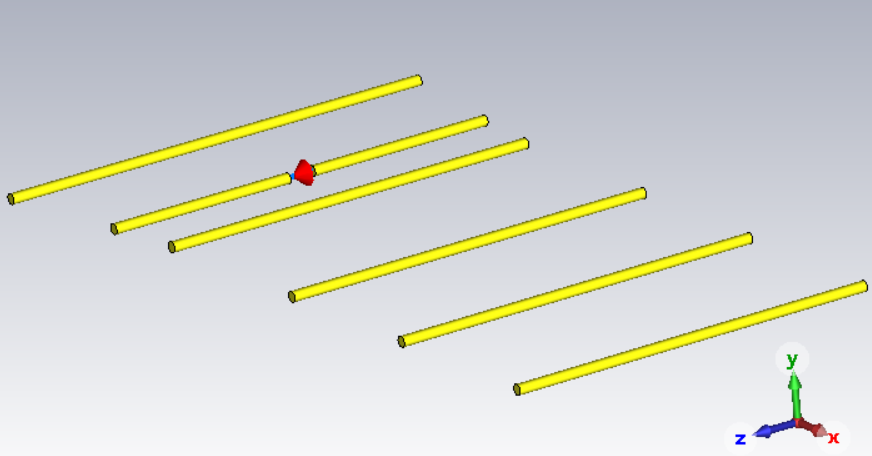
\includegraphics[width=0.9\linewidth]{Imagens/CST_Antenna.png}
\caption{Yagi-Uda antenna simulated in CST Studio Suite.}
\label{cap3:sec6:fig1}
\end{figure}

\subsection{Simulation and Dimensions}

The optimised element lengths and spacings obtained in CST Studio Suite are given in Table~\ref{cap3:sec6:table1}\protect\footnotemark\footnotetext{The reference position is measured from the midpoint between the two halves of the driven dipole element. The boom is aligned with the central axis of the elements.}, and the constructed prototype is shown in Figure~\ref{cap3:sec6:fig2: b}. 
Two identical Yagi-Uda antennas were constructed based on these specified dimensions: one dedicated to transmission and the other to reception. This configuration enabled testing the antenna performance within a representative communication link scenario.


\begin{table}[H]
\centering
\caption{Element lengths and spacings for the Yagi-Uda antenna.}
\label{cap3:sec6:table1}
\begin{tabular}{lcc}
\hline
Element & Length (mm) & Position (mm) \\
\hline
Reflector & 166.41 & -51.964 \\
Driven & 150.98 & 0.0 \\
Director 1 & 143.85 & 30.104 \\
Director 2 & 142.16 & 102.131 \\
Director 3 & 140.48 & 166.814 \\
Director 4 & 139.51 & 234.902 \\
\hline
\end{tabular}
\end{table}


\subsection{Building the Yagi-Uda Antenna}
\label{cap3:sec6:subsec2:build_antenna}

The antenna was modelled mechanically in SolidWorks\footnote{Educational version licensed to the Polytechnic Institute of Bragança.} (Figure~\ref{cap3:sec6:fig2: a}) and the boom was fabricated using fused deposition modelling (FDM) with PLA, as shown in Figure \ref{cap3:sec6:fig2: b}. The radiating elements were made from solid brass rods with a diameter of 3\,mm\footnote{Brass composition was approximately two-thirds copper and one-third zinc.}. %, with conductivity $\sigma = 15.9 \times 10^{6}$\,S/m and thickness $d = 0.68 \times 10^{-3}$\,m.%



\begin{figure}[H]
     \centering
     \begin{subfigure}{0.552\textwidth}
         \centering
         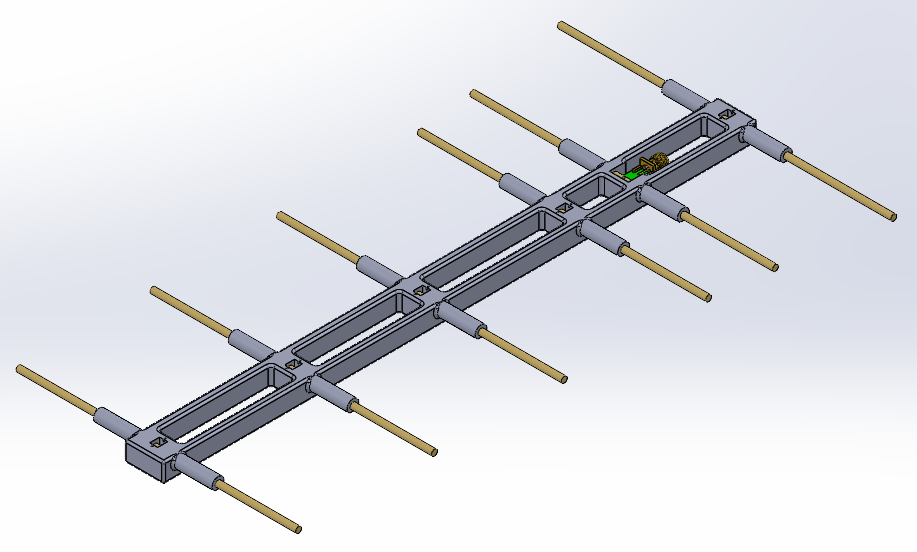
\includegraphics[width=\textwidth]{Imagens/Solidworks_antena.png}
         \caption{Mechanical model in SolidWorks}
         \label{cap3:sec6:fig2: a}
     \end{subfigure}
     \hspace{1mm}
     \begin{subfigure}{0.405\textwidth}
         \centering
         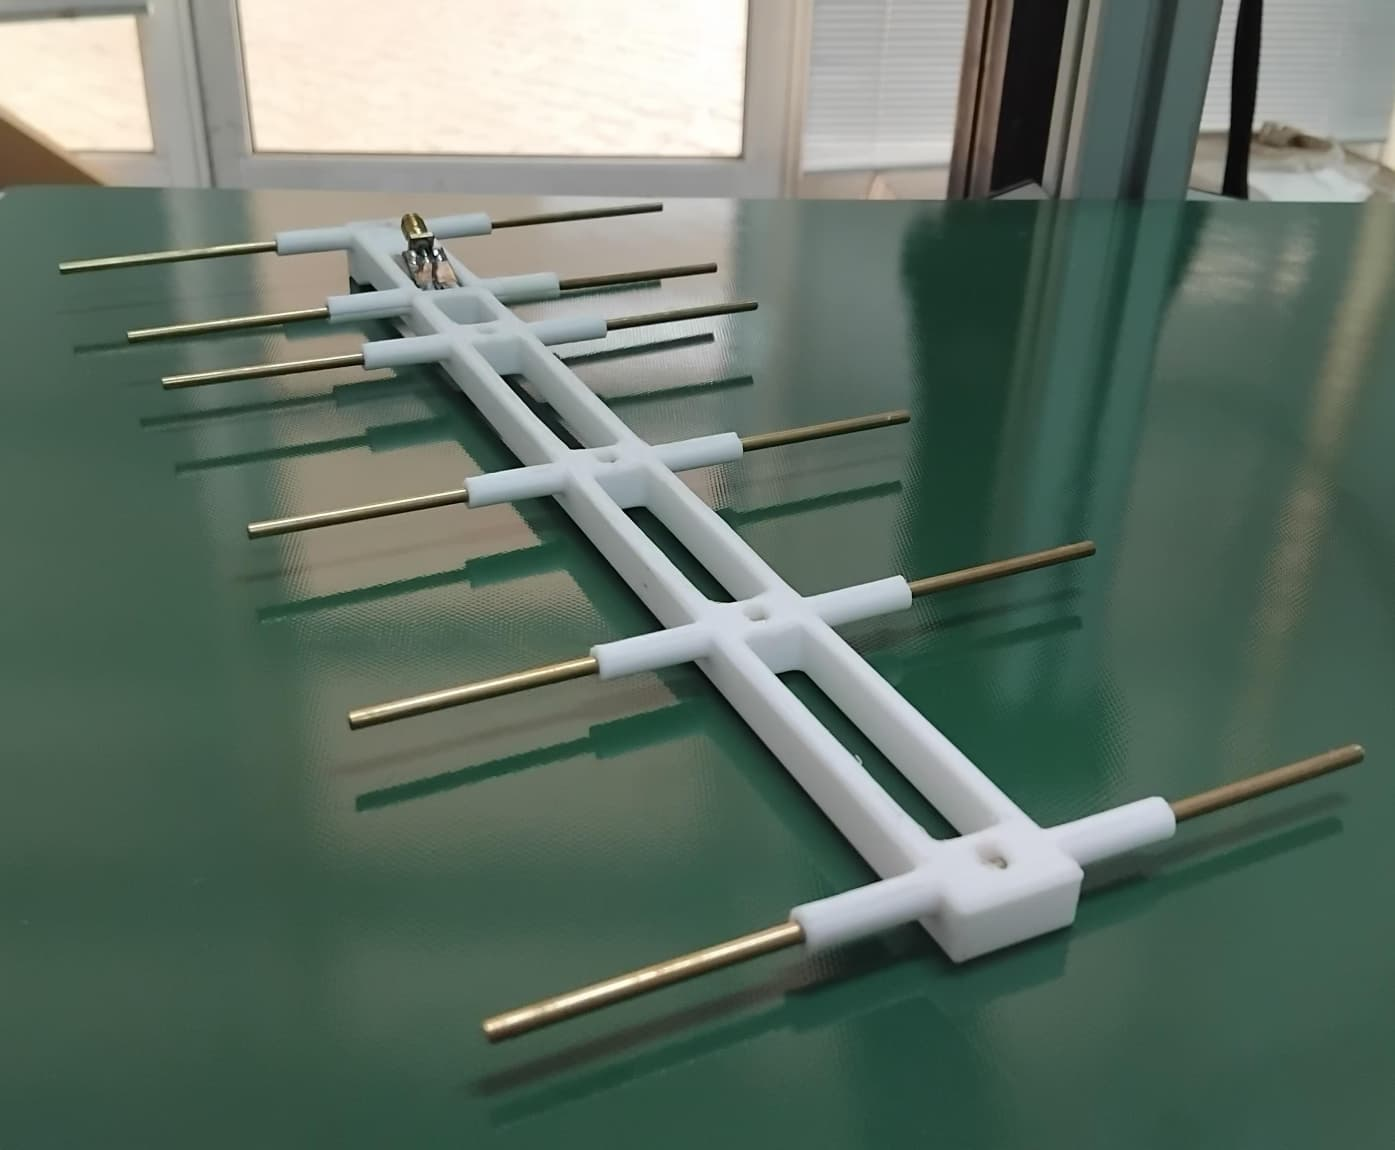
\includegraphics[width=\textwidth]{Imagens/antenna_prototype.jpeg}
         \caption{Constructed prototype}
         \label{cap3:sec6:fig2: b}
     \end{subfigure}
        \caption{Mechanical model of the antenna developed in SolidWorks and the constructed Yagi-Uda antenna prototype.}
        \label{cap3:sec6:fig2}
\end{figure}


%-----------------------------------------------------------------------------------------------------
\subsection{Antenna Characterisation}
\label{cap3:sec6:subsec3}
%-----------------------------------------------------------------------------------------------------

The reflection coefficient $S_{11}$ and the VSWR of the transmitting and receiving antennas were measured with the NanoVNA. both antennas exhibited nearly identical responses, as expected from their close design, with only minor construction tolerances causing negligible deviations; therefore, only one set of results is presented in Figure~\ref{cap3:sec6:subsec3:fig1} for conciseness. Minor variations between them are expected due to construction tolerances, but no significant deviations were observed.

The resonance occurs close to the intended frequency of 868~MHz. The optimum impedance matching condition was obtained at approximately 876~MHz, where $S_{11}$ reached around $-13$~dB and the VSWR was 1.58. At 868~MHz, the measured values were $S_{11} \approx -11$~dB and VSWR $\approx 1.77$, corresponding to an input impedance of about $30 + j0.7~\Omega$. The $-10$~dB bandwidth extends from 865~MHz to 890~MHz, resulting in approximately 25~MHz, which is consistent across both NanoVNA and QucsStudio measurements.

\begin{figure}[H]
    \centering
    \begin{subfigure}{0.99\textwidth}
        \centering
        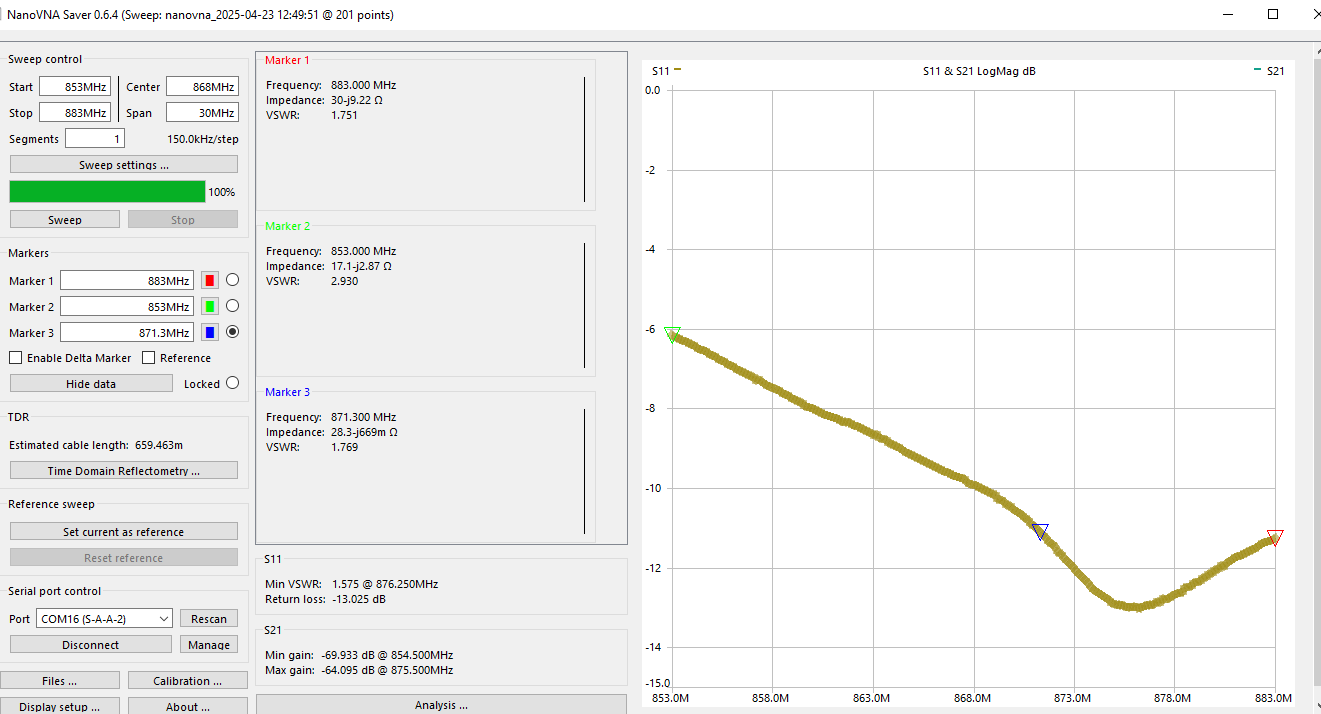
\includegraphics[width=\textwidth]{Imagens/Antena Transmissora/Caraterização VNA/Fig2.png}
        \caption{$S_{11}$}
        \label{cap3:sec6:subsec3:fig1:a}
    \end{subfigure}
    \hfill
    \begin{subfigure}{0.99\textwidth}
        \centering
        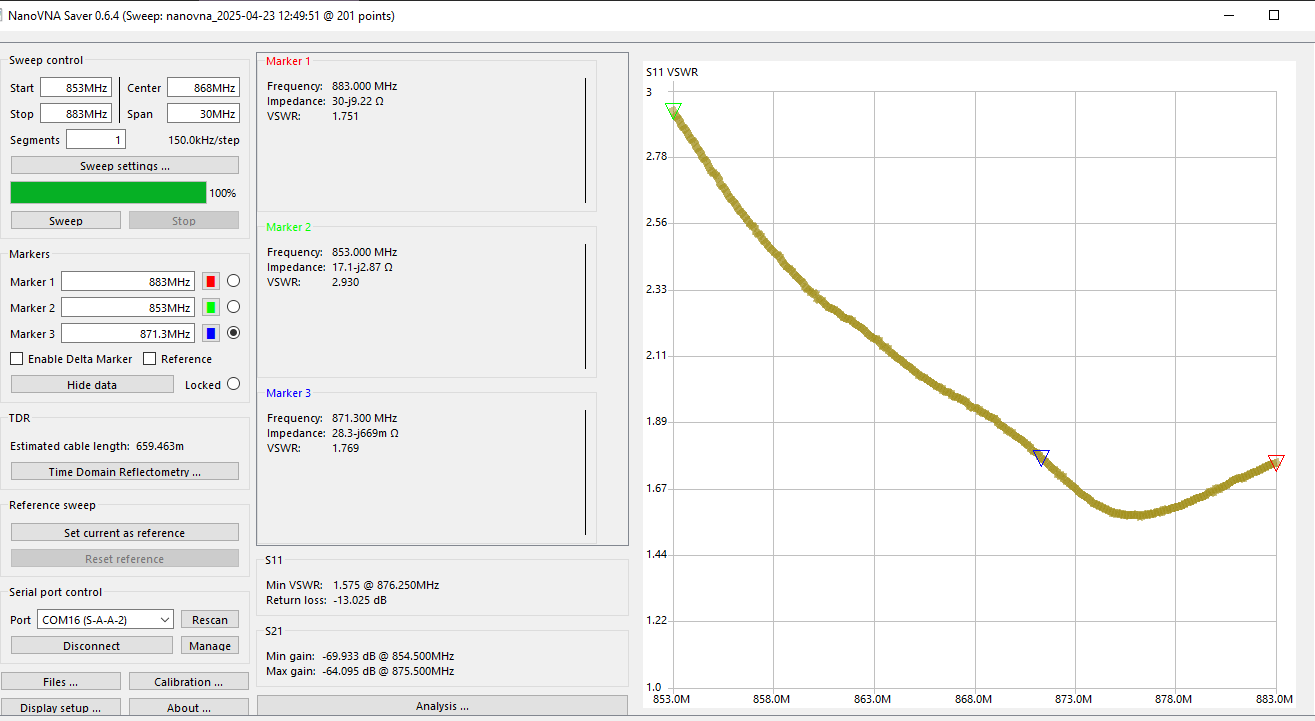
\includegraphics[width=\textwidth]{Imagens/Antena Transmissora/Caraterização VNA/Fig4.png}
        \caption{VSWR}
        \label{cap3:sec6:subsec3:fig1:b}
    \end{subfigure}
    \caption{Characterisation of the antenna using the NanoVNA.}
    \label{cap3:sec6:subsec3:fig1}
\end{figure}

Overall, the antennas demonstrate acceptable matching around the ISM band, validating their suitability for the subsequent radiation pattern measurements. Nevertheless, clearly could be better parameters.

%-----------------------------------------------------------------------------------------------------
\section{RF Signal Integrity: Balun and Impedance Matching Network}
\label{sec:Balun_Impedance-matching}
%-----------------------------------------------------------------------------------------------------

In RF systems, optimal power transfer and signal integrity depend not only on the antenna geometry but also on suppressing undesired current modes and ensuring accurate impedance matching between interconnected components \cite{balanis2016}. Since the nominal characteristic impedance of most RF systems is $50,\Omega$, particular attention was given to this requirement during the antenna design.

Therefore, two strategies were  implemented: (i) mitigation of common-mode currents through the use of a balun, and (ii) the design of an impedance matching network to ensure a $50\,\Omega$ interface between the antenna and the transmission line, as well the RF sensor module.

\subsection{Balun for Common-Mode Current Suppression}

When a balanced antenna, such as the Yagi-Uda, is connected to an unbalanced coaxial transmission line, common-mode currents can propagate along the shield of the coaxial cable. These currents can cause radiation from the feed line itself, altering the antenna radiation pattern and impedance characteristics \cite{Fiorelli2011,Icheln2004}. To mitigate this effect, a current balun was implemented, functioning as a choke to suppress common-mode currents without affecting the desired differential-mode signal \cite{Duffy2022, Sevick2001}.

The balun geometry was designed using analytical calculations that considered the type of coaxial cable (RG-174) and its physical dimensions, as the conductor diameter and dielectric properties directly influence the inductance, the skin effect, and the ability to suppress common-mode currents at RF. A MATLAB script was used to determine the optimal number of turns and winding diameter for operation at the target frequency\footnote{The MATLAB script in Appendix~\ref{apendice5} was used for the geometric design of the balun.}.\\
\vspace{0.1em}
\indent The design and evaluation stages included both simulation and measurement. After confirming through VNA measurements, as seen in Figure \ref{fig:balun_fotos_all}, that the geometry provided effective suppression, the balun was manufactured as illustrated in Figure~\ref{cap3:sec7:fig1}.

\begin{figure}[H]
    \centering
    % Esquerda: imagem grande
    \begin{subfigure}[b]{0.482\textwidth}
        \centering
        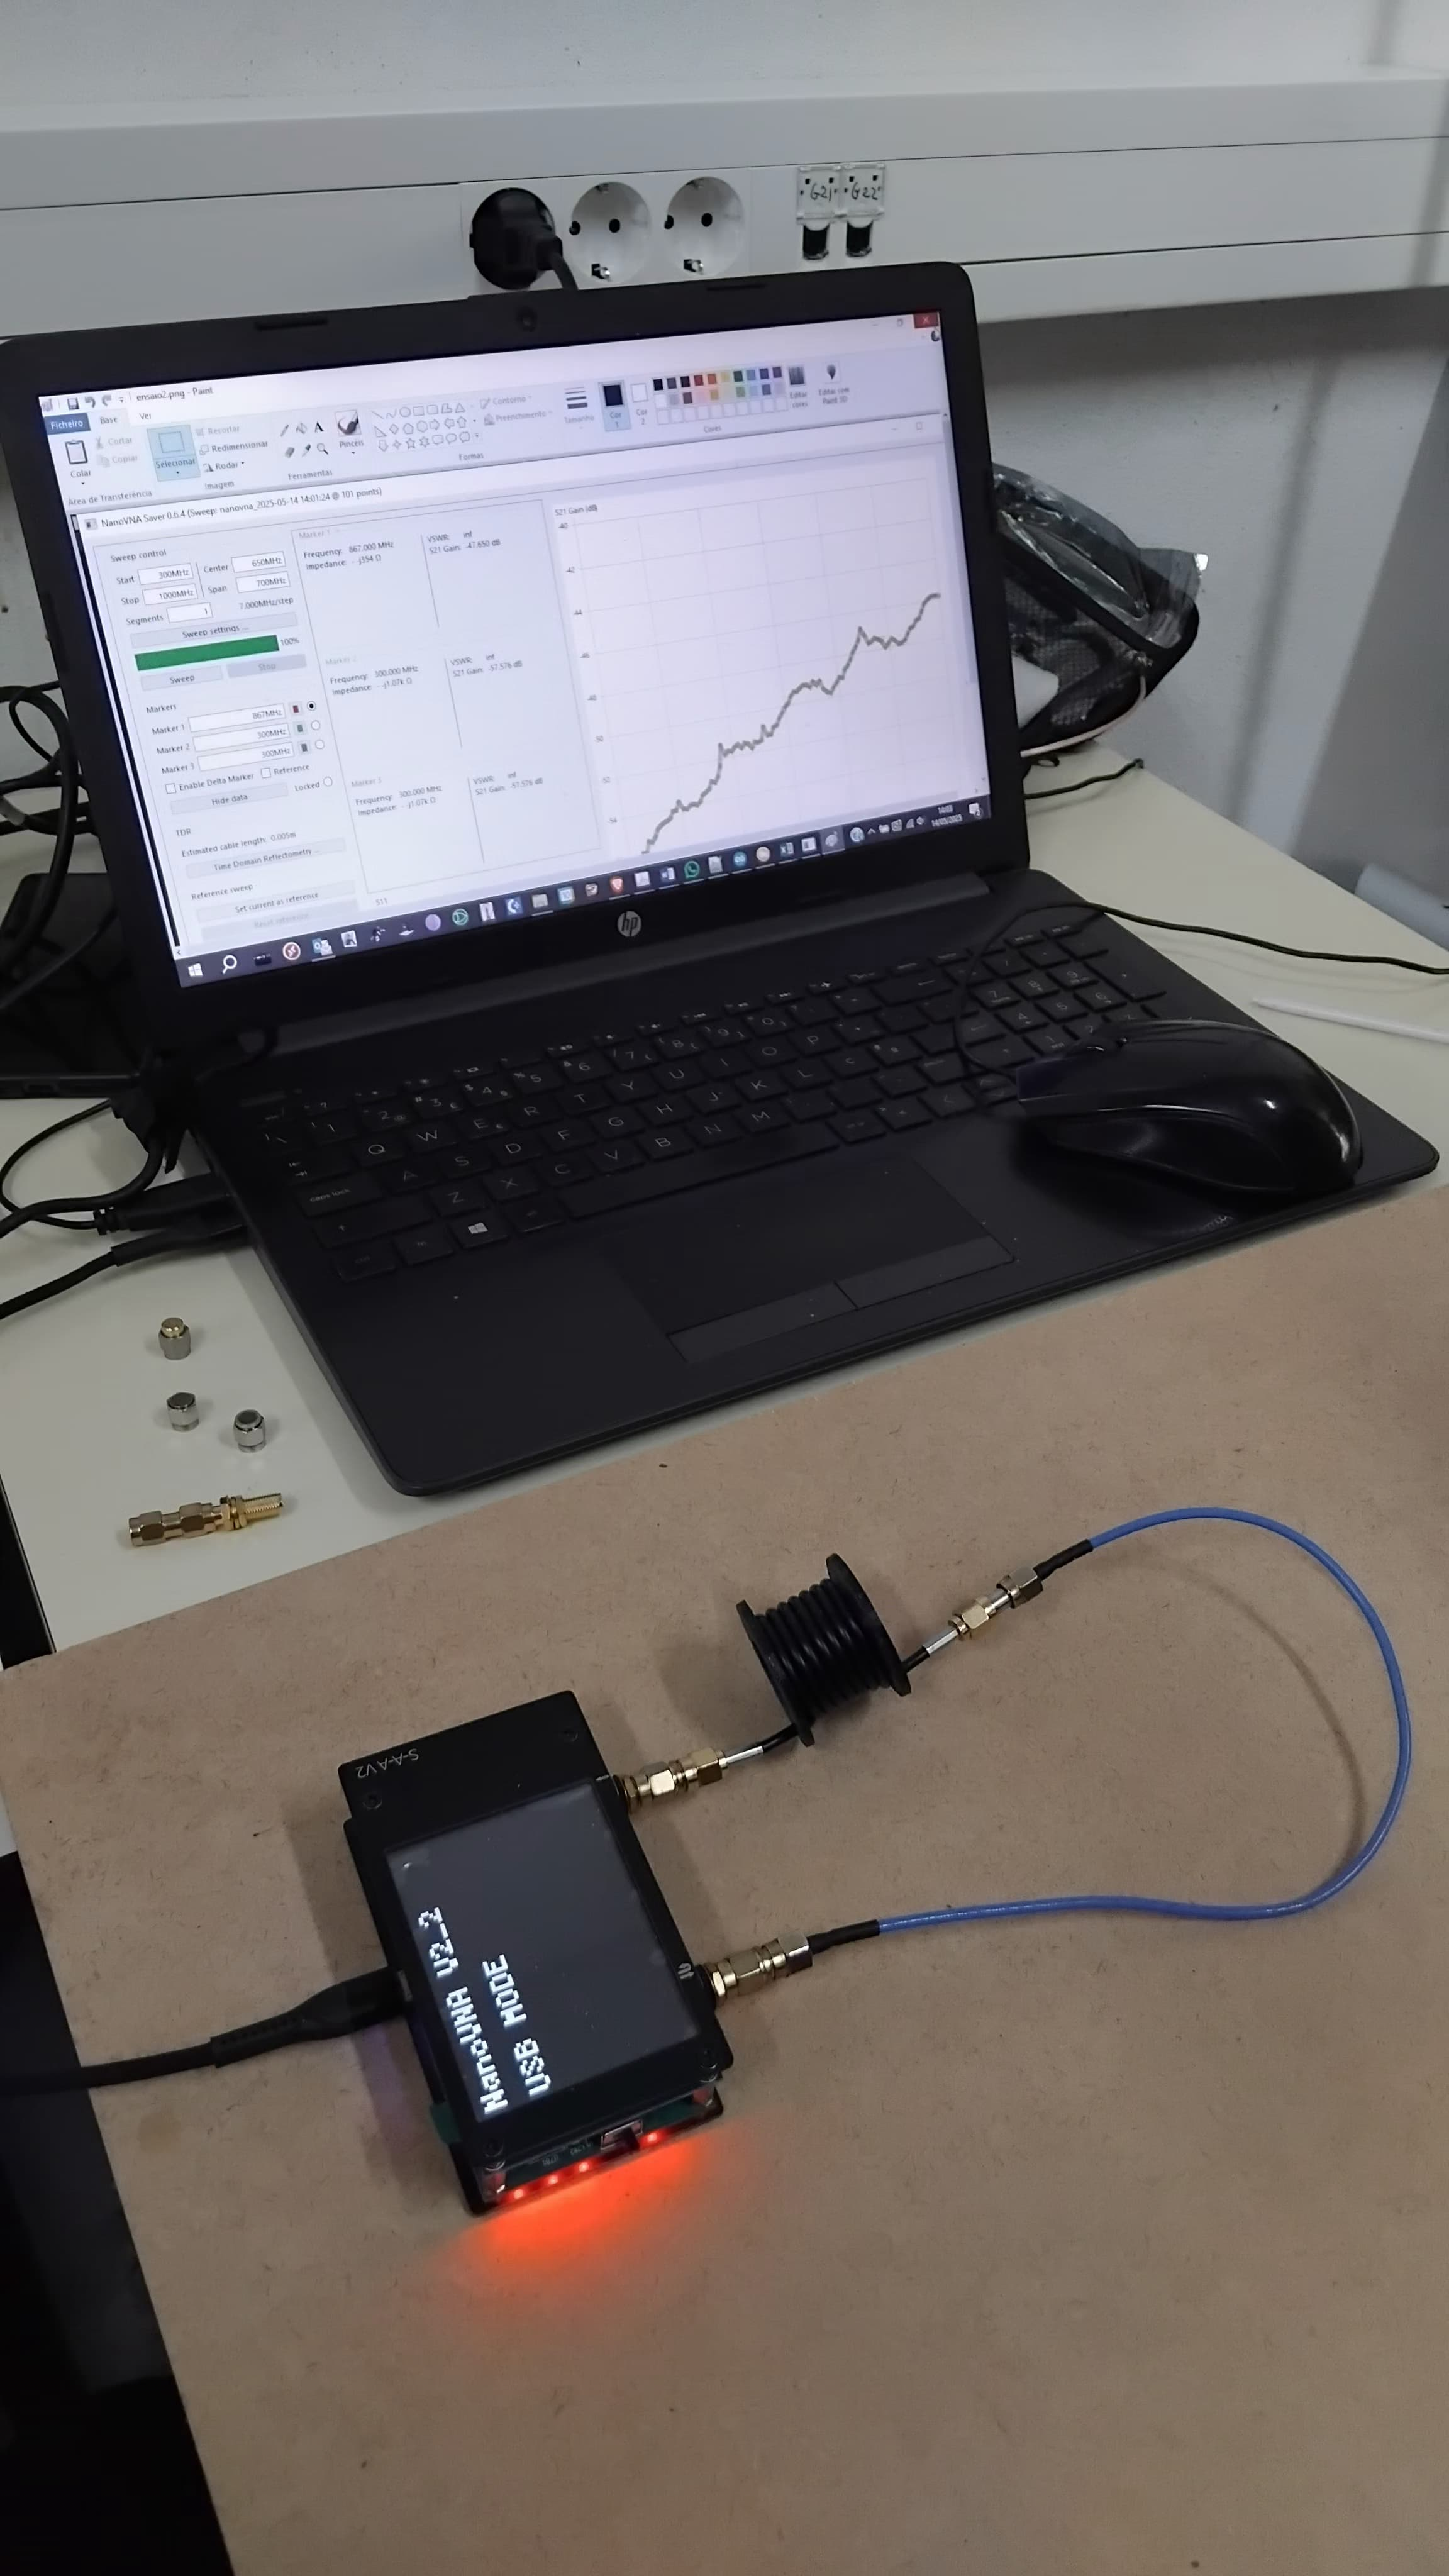
\includegraphics[width=\textwidth]{Imagens/balun3.jpg}
        \caption{Balun during characterisation.}
        \label{fig:balun_foto_lateral}
    \end{subfigure}
    \hspace{2mm}
    % Direita: duas imagens menores empilhadas
    \begin{subfigure}[b]{0.48\textwidth}
        \centering
        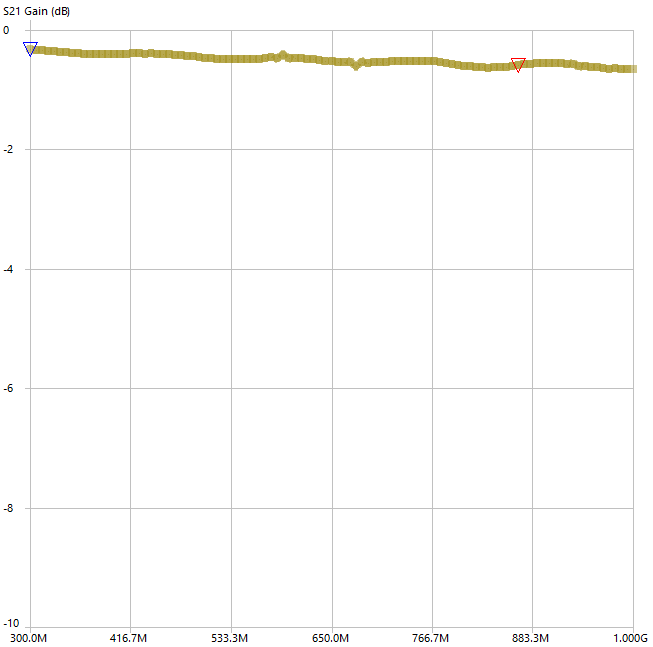
\includegraphics[width=0.845\textwidth]{Imagens/balun_caract/insertion_loss.png}
        \caption{Differential mode.}
        \label{fig:balun_foto_regua}
        \vskip 2mm
        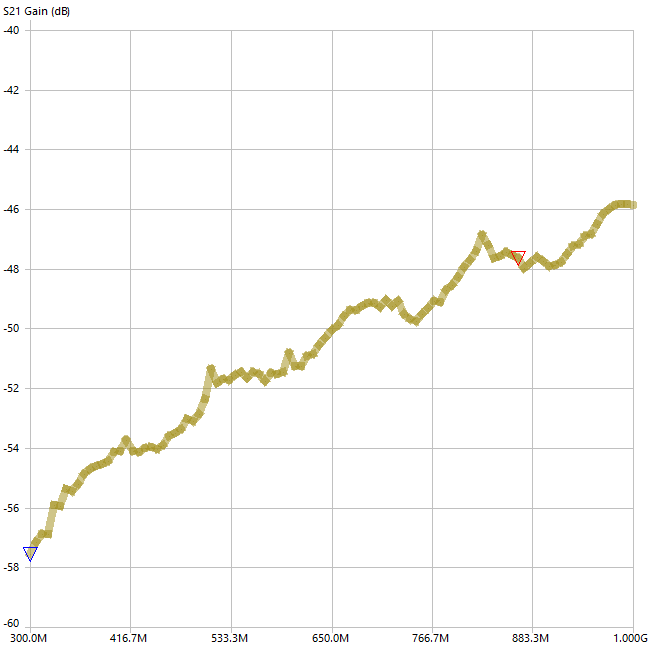
\includegraphics[width=0.845\textwidth]{Imagens/balun_caract/insertion_loss2.png}
        \caption{Common mode.}
        \label{fig:balun_foto_superior}
    \end{subfigure}
    \caption{Characterisation of the air choke balun.}
    \label{fig:balun_fotos_all}
\end{figure}

\begin{figure}[H]
    \centering
    \begin{subfigure}{0.427\textwidth}
        \centering
        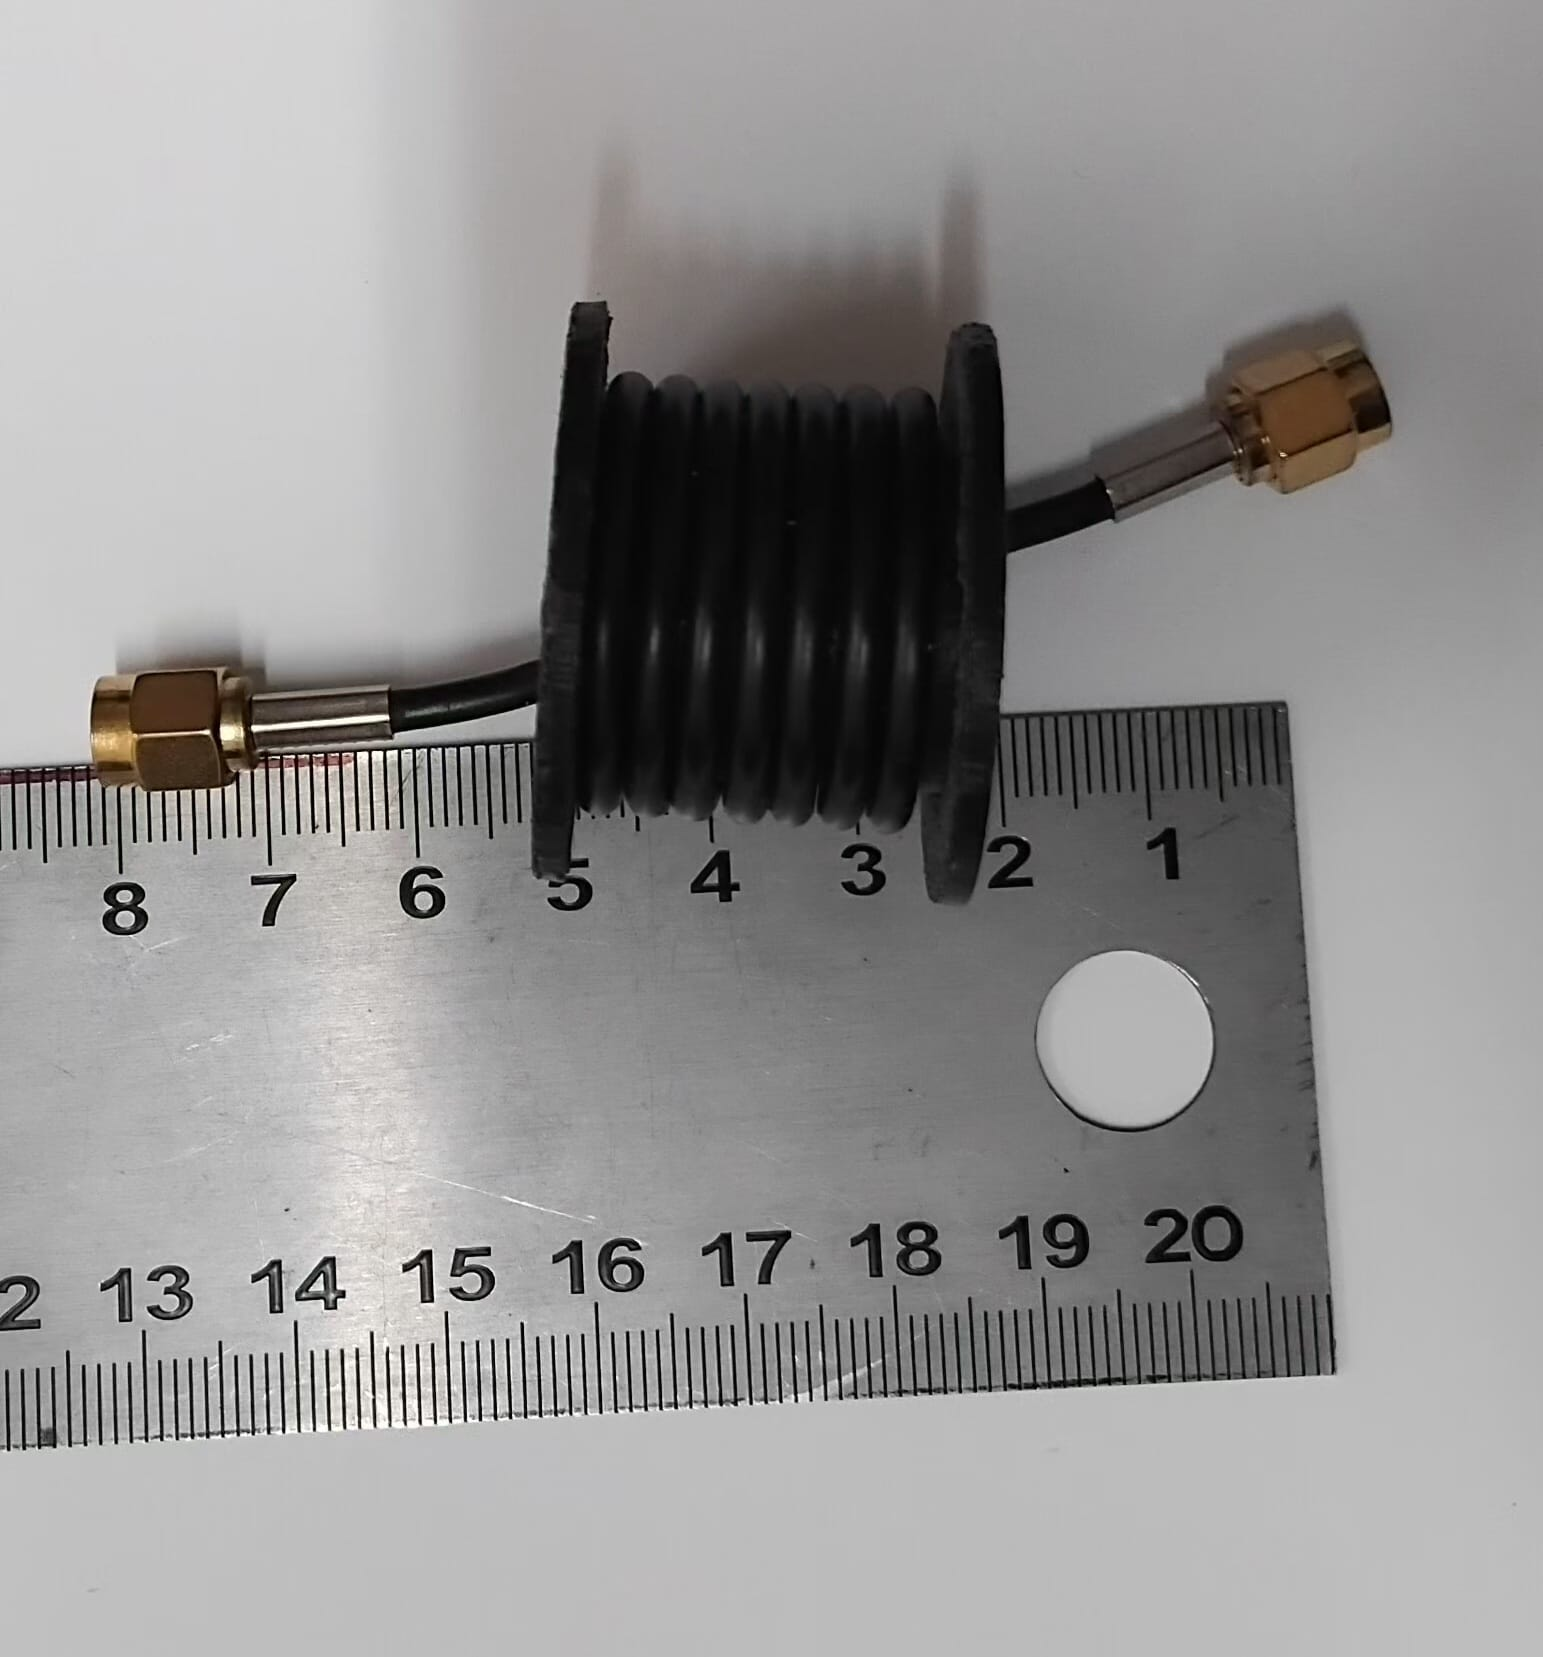
\includegraphics[width=\textwidth]{Imagens/balun.jpg}
        \caption{Balun and a measuring tape.}
        \label{cap3:sec7:fig1:a}
    \end{subfigure}
    \hspace{1mm}
    \begin{subfigure}{0.4875\textwidth}
        \centering
        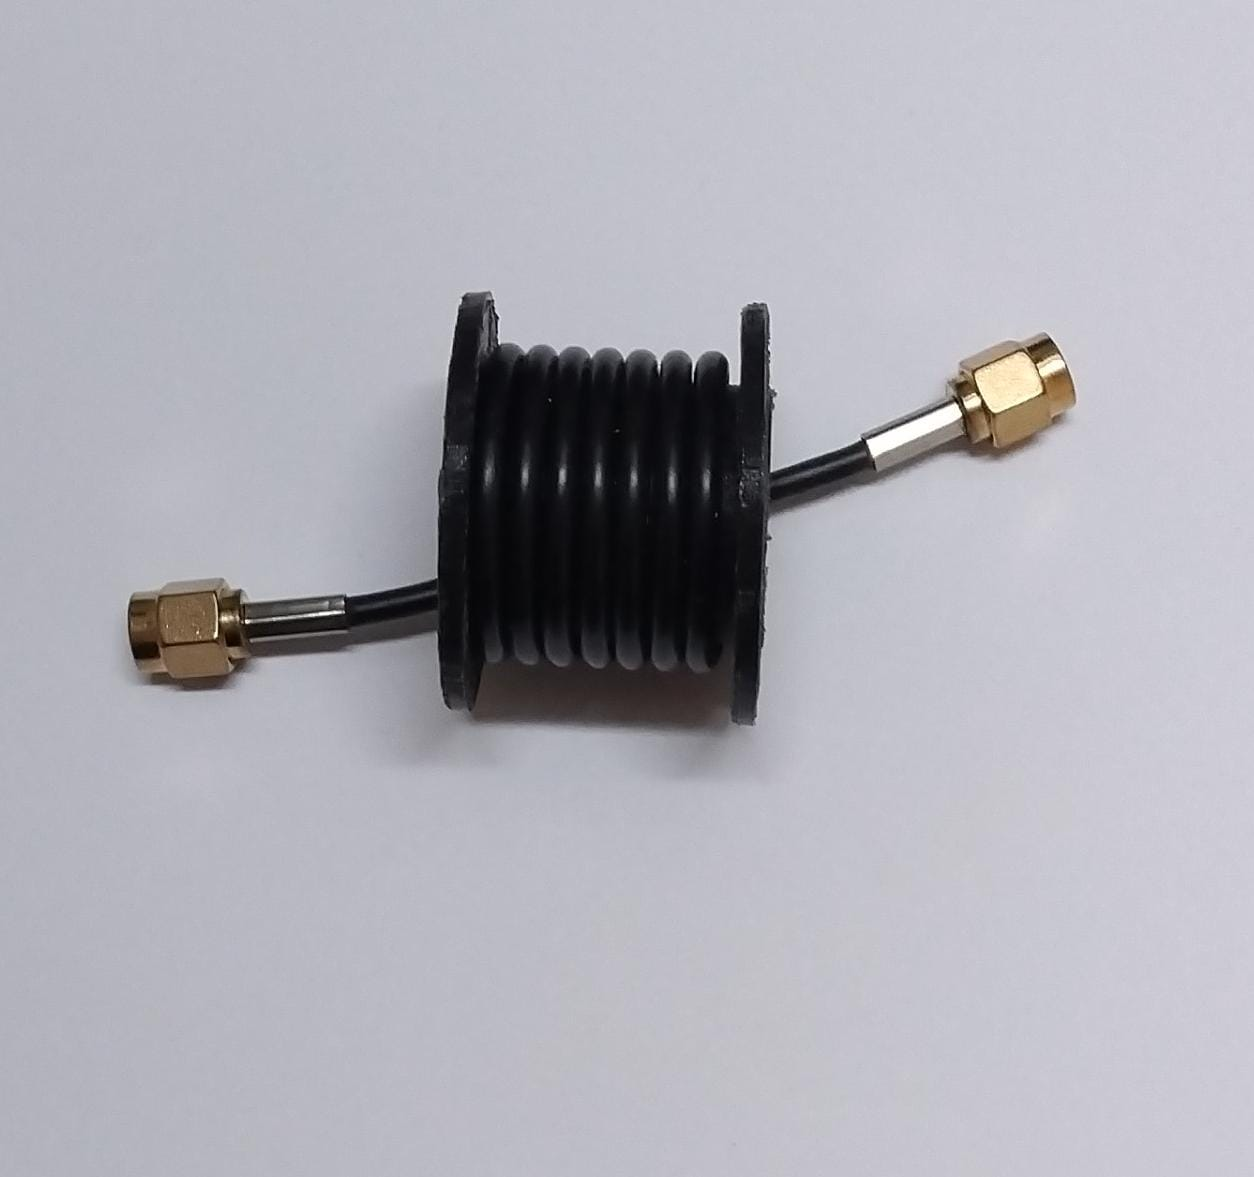
\includegraphics[width=\textwidth]{Imagens/balun2.jpg}
        \caption{Top view of the balun.}
        \label{cap3:sec7:fig1:b}
    \end{subfigure}
    \caption{Photos of the air choke balun manufactured using RG174 cable, with 3D printed support.}
    \label{cap3:sec7:fig1}
\end{figure}

%-----------------------------------------------------------------------------------------------
\subsection{Impedance Matching Network Design}
%-----------------------------------------------------------------------------------------------


After antenna characterisation, as seen in Subsection~\ref{cap3:sec6:subsec3}, it became evident that impedance matching was required due to the observed mismatch with the $50\,\Omega$ reference\cite{ARRL2023}. Initial estimates for the matching network components (capacitor and inductor) were obtained using QucsStudio and CST simulations, considering the antenna response alone. However, these values needed refinement once the effect of the PCB layout was included. For this reason, the PCB was first characterised in its bare form, without components, to quantify its intrinsic parasitic contributions.

The shunt PCB impedance, $|Z| \approx 21.5~\Omega$, was obtained from the measured $S_{21}$, as shown in Figure \ref{fig:pcb_s21_curve}. Then, the corresponding parasitic capacitance follows from Equation~\eqref{eq:capacitance_from_impedance}. This measurement yielded $C \approx 8.5~\text{pF}$. Simulations independent of the PCB (CST and QucsStudio) gave $C \approx 7.8~\text{pF}$, in close agreement with the experimental result. Figures \ref{fig:cst_results} and \ref{fig:qucs_results} show the models and results obtained from the simulations.


\begin{figure}[H]
    \centering
    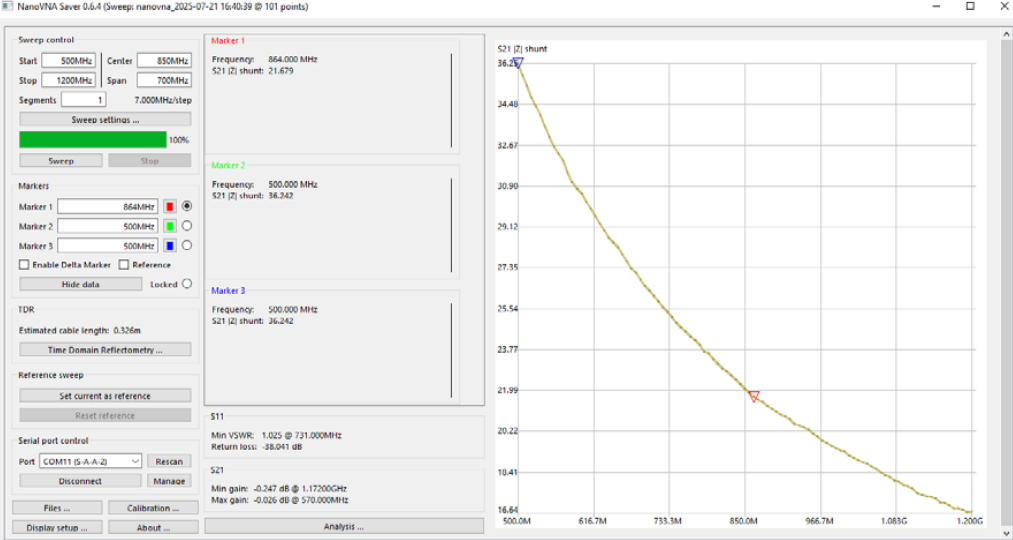
\includegraphics[width=0.75\linewidth]{Imagens/NanoVNA_PCB_S21.png}
    \caption{Measured $S_{21}$ curve of the bare PCB with NanoVNA Saver.}
    \label{fig:pcb_s21_curve}
\end{figure}


\begin{align}
C &= \frac{1}{2 \pi f |Z|} \label{eq:capacitance_from_impedance} = \frac{1}{2 \pi \cdot (868 \times 10^{6}) \cdot 21.5}
\approx 8.5~\text{pF}
\end{align}

\begin{figure}[H]
    \centering
    \begin{subfigure}{0.8\textwidth}
        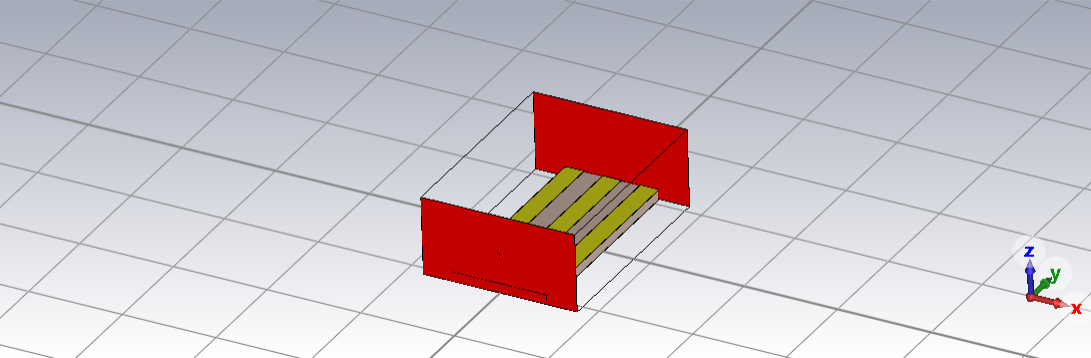
\includegraphics[width=\linewidth]{Imagens/CST_Model.png}
        \caption{CST PCB model}
        \label{fig:cst_model}
    \end{subfigure}\hfill
    \begin{subfigure}{0.8\textwidth}
        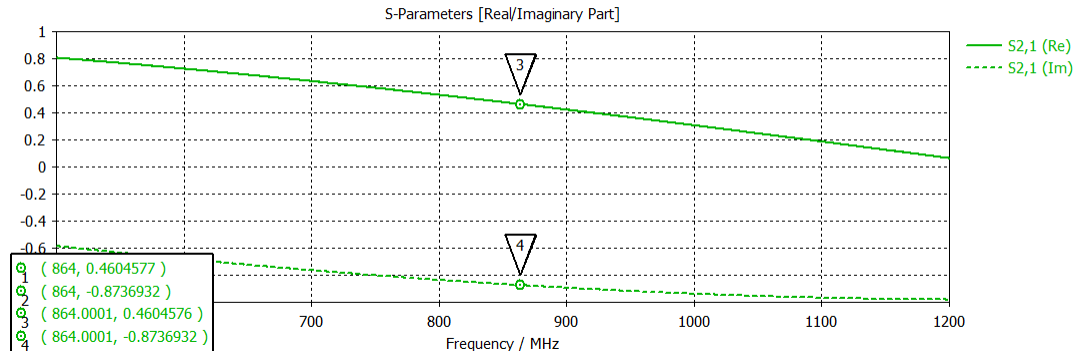
\includegraphics[width=\linewidth]{Imagens/CST_Results.png}
        \caption{CST simulation result}
        \label{fig:cst_resultb}
    \end{subfigure}
    \caption{CST Studio Suite simulation of the PCB}
    \label{fig:cst_results}
\end{figure}

\begin{figure}[H]
    \centering
    \begin{subfigure}{0.85\textwidth}
        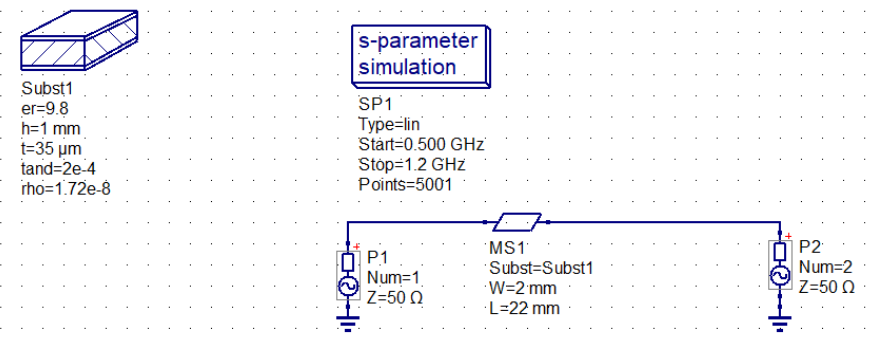
\includegraphics[width=\linewidth]{Imagens/Qucs_Model.png}
        \caption{QucsStudio PCB model}
        \label{fig:qucs_model}
    \end{subfigure}\hfill
    \begin{subfigure}{0.75\textwidth}
        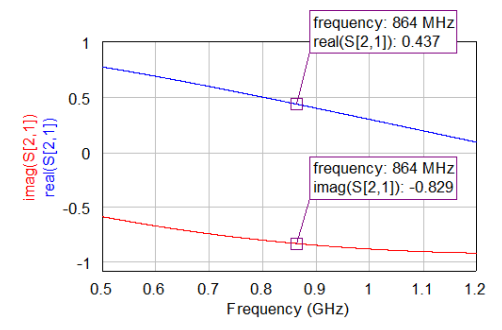
\includegraphics[width=\linewidth]{Imagens/Qucs_Results.png}
        \caption{QucsStudio simulation result}
        \label{fig:qucs_result}
    \end{subfigure}
    \caption{QucsStudio simulation of the PCB: (a) model and (b) result.}
    \label{fig:qucs_results}
\end{figure}

\begin{equation}
Z = Z_0 \cdot \frac{S_{21}}{2(1 - S_{21})}, \quad Z_0 = 50~\Omega
\label{eq:impedance_from_s21}
\end{equation}

\begin{equation}
Z_{\text{CST}} = 50 \cdot \frac{0.460458 - j0.873693}{2\left(1 - (0.460458 - j0.873693)\right)}
\approx -12.21 - j20.71~\Omega
\label{eq:Z_CST}
\end{equation}

\begin{equation}
|Z_{\text{CST}}| = \sqrt{(-12.21)^2 + (-20.71)^2} \approx 24.04~\Omega
\label{eq:Z_CST_module}
\end{equation}

\begin{align}
C_{\text{CST}} &= \frac{1}{2 \pi \cdot 864 \times 10^{6} \cdot 24.04} \label{eq:C_CST} \\
C_{\text{CST}}&\approx 7.66 \times 10^{-12}\ \text{F}\\
C_{\text{CST}}&= 7.66~\text{pF}
\end{align}

\begin{align}
Z_{\text{Qucs}} &= 50 \cdot \frac{0.437 - j0.829}{2\left(1 - (0.437 - j0.829)\right)} \label{eq:Z_QUCS} \\
Z_{\text{Qucs}}&\approx -10.98 - j20.64~\Omega
\end{align}

\begin{equation}
|Z_{\text{Qucs}}| = \sqrt{(-10.98)^2 + (-20.64)^2} \approx 23.38~\Omega
\label{eq:Z_QUCS_module}
\end{equation}

\begin{align}
C_{\text{Qucs}} &= \frac{1}{2 \pi \cdot 864 \times 10^{6} \cdot 23.38} \label{eq:C_QUCS} \\
C_{\text{Qucs}}&\approx 7.87 \times 10^{-12}\ \text{F} \\
C_{\text{Qucs}}&= 7.87~\text{pF}
\end{align}

\vspace{0.1em}
\indent As noted, the results of the measurements and simulations (CST and QucsStudio) are in close agreement, producing parasitic capacitance values in the range of $7.66$ to $8.5$ pF. This consistency confirms that the PCB introduces significant capacitance, which would be an issue if it was not considered for the impedance matching design\cite{Saario2003}.\\
\vspace{0.1em}
\indent After, all S-parameters were acquired to build a Touchstone file of the PCB for co-simulation with the DUT. With the NanoVNA, the sweep was performed to obtain $S_{11}$ and $S_{21}$, and the ports were inverted to acquired the $S_{22}$ and $S_{12}$. Then, they were merged into a single two-port file. The measured responses are shown in Figure~\ref{fig:pcb_full_sparams}, while the resulting files were validated in Qucs before use, is illustrated in Figure~\ref{fig:touchstone}.

\begin{figure}[H]
    \centering
    \begin{subfigure}{0.49\textwidth}
        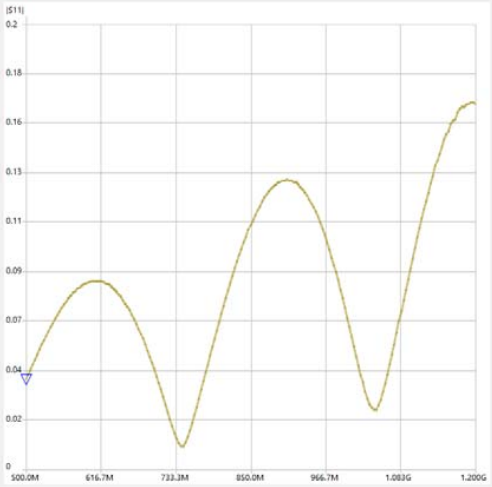
\includegraphics[width=\linewidth]{Imagens/NanoVNA_S11.png}
        \caption{Measured $S_{11}$}
        \label{fig:pcb_s11}
    \end{subfigure}
    \hfill
    \begin{subfigure}{0.49\textwidth}
        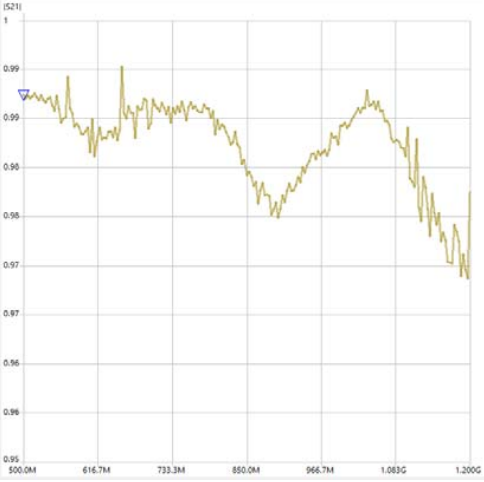
\includegraphics[width=\linewidth]{Imagens/NanoVNA_S21.png}
        \caption{Measured $S_{21}$}
        \label{fig:pcb_s21}
    \end{subfigure}
    \vskip 2mm
    \begin{subfigure}{0.49\textwidth}
        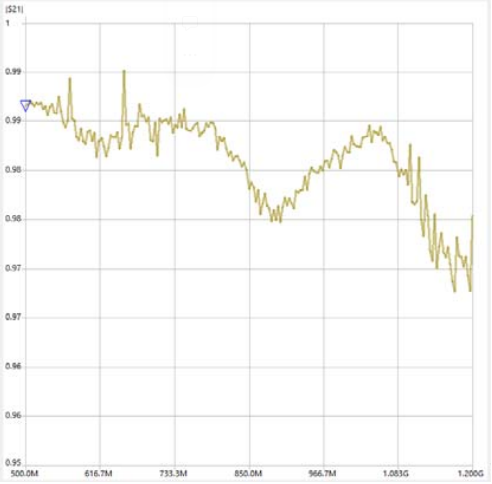
\includegraphics[width=\linewidth]{Imagens/NanoVNA_S12.png}
        \caption{Measured $S_{12}$}
        \label{fig:pcb_s12}
    \end{subfigure}
    \hfill
    \begin{subfigure}{0.49\textwidth}
        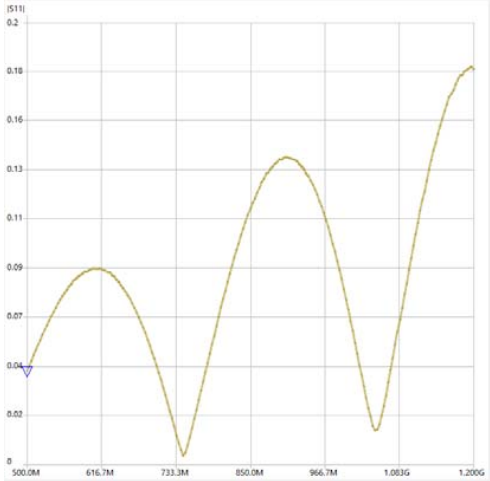
\includegraphics[width=\linewidth]{Imagens/NanoVNA_S22.png}
        \caption{Measured $S_{22}$}
        \label{fig:pcb_s22}
    \end{subfigure}
    \caption{Measured S-parameters of the PCB using NanoVNAsaver.}
    \label{fig:pcb_full_sparams}
\end{figure}



\begin{figure}[H]
    \centering
    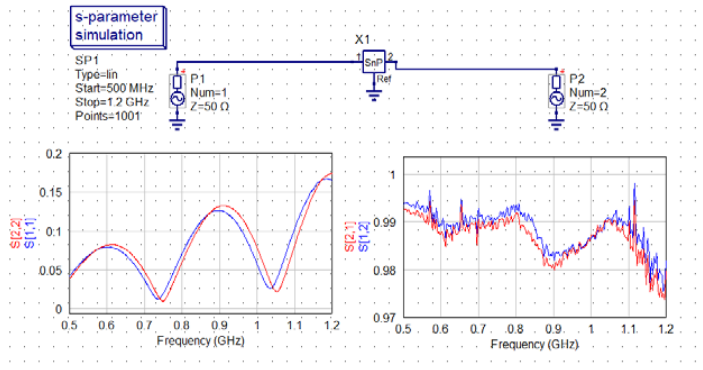
\includegraphics[width=0.9\linewidth]{Imagens/touchstone_validation.png}
    \caption{Validation of the Touchstone file in QucsStudio.}
    \label{fig:touchstone}
\end{figure}

When the PCB Touchstone model was combined with the antenna, a deterioration of the VSWR was observed, confirming the parasitic loading effect, as shown in Figure \ref{cap3:sec6:fig1585}. An updated matching network was therefore designed to restore the input impedance close to $50\,\Omega$. Figure~\ref{fig:matching_results} compares the results obtained in QucsStudio and SimNEC after optimisation.

\begin{figure}[H]
\centering
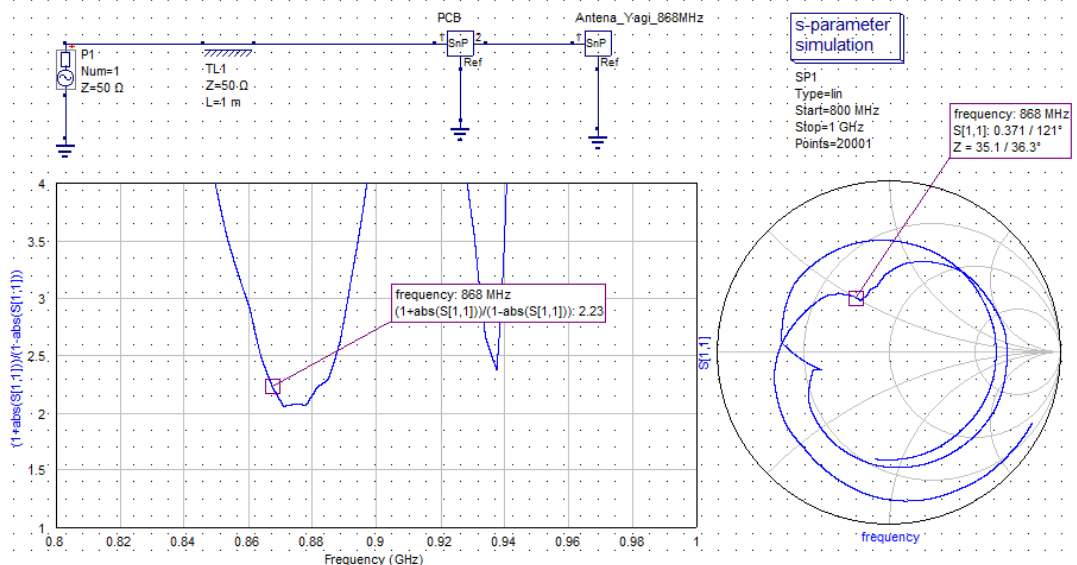
\includegraphics[width=0.9\linewidth]{Imagens/antena antes.png}
\caption{before impedance matching network.}
\label{cap3:sec6:fig1585}
\end{figure}

\begin{figure}[H]
    \centering
    \begin{subfigure}{0.8\textwidth}
        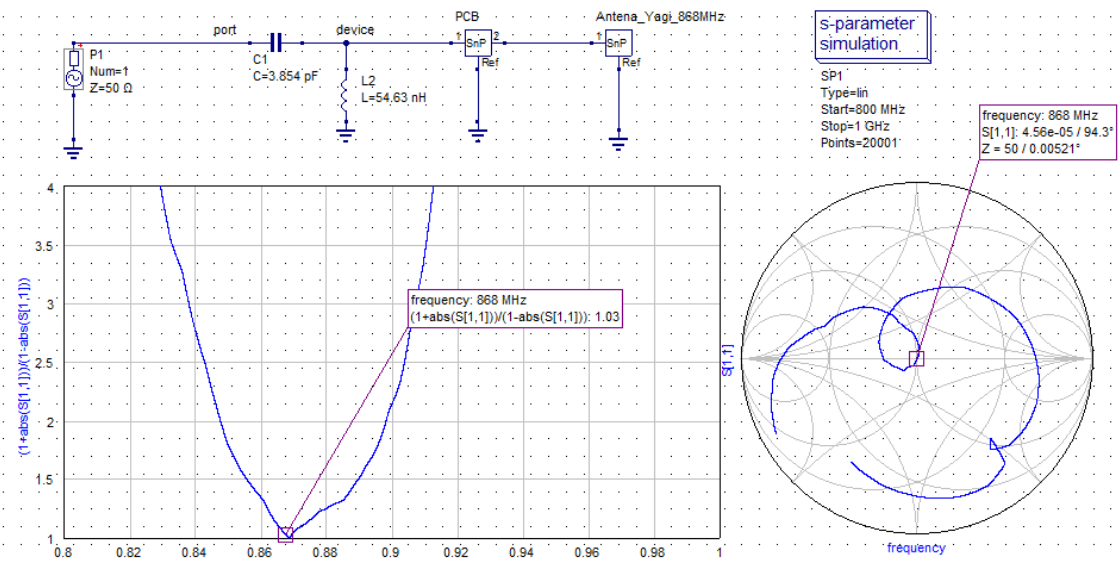
\includegraphics[width=\linewidth]{Imagens/antena depois.png}
        \caption{Impedance matching in QucsStudio.}
    \end{subfigure}\hfill
    \begin{subfigure}{0.8\textwidth}
        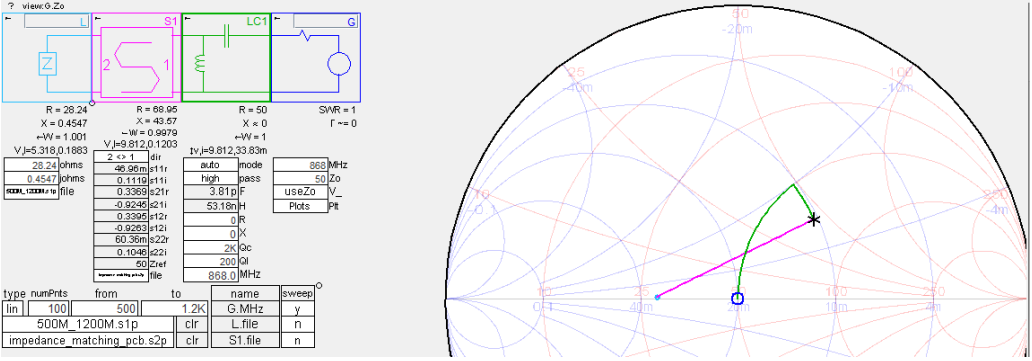
\includegraphics[width=\linewidth]{Imagens/Simnec_Matching.png}
        \caption{Matching network validation in SimNEC.}
    \end{subfigure}
    \caption{Results of the optimised matching network.}
    \label{fig:matching_results}
\end{figure}

The final values of network component are listed in Table~\ref{tab:lc_values}. These elements were used in the manufactured PCB.

\begin{table}[H]
\centering
\caption{Final LC matching network component values.}
\label{tab:lc_values}
\begin{tabular}{|l|c|c|}
\hline
Element & Estimated & Used \\ \hline
$L$     & 54.6~nH   & 56~nH \\ \hline
$C$     & 3.8~pF    & 3.9~pF \\ \hline
\end{tabular}
\end{table}


Finally, Figure~\ref{cap3:sec7:fig3} shows the complete PCB design workflow: (a) layout model in QucsStudio, (b) schematic design in EasyEDA\footnote{EasyEDA is a free, online PCB design software.}, and (c) the manufactured board.

\begin{figure}[H]
    \centering
    \begin{subfigure}{\textwidth}
        \centering
        \fbox{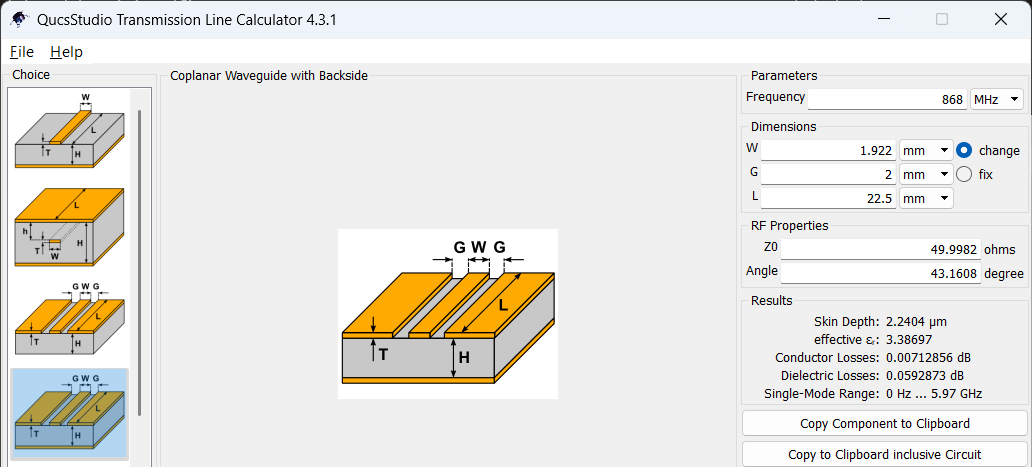
\includegraphics[width=0.6\linewidth]{Imagens/calculo da placa.png}}
        \caption{QucsStudio PCB layout model}
        \label{cap3:sec7:fig3:a}
    \end{subfigure}
    \vskip 2mm
    \begin{subfigure}{\textwidth}
        \centering
        \fbox{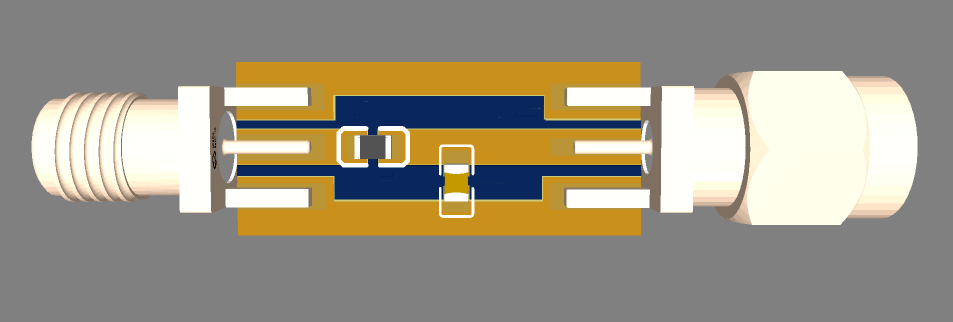
\includegraphics[width=0.6\linewidth]{Imagens/PCB3.png}}
        \caption{PCB design in EasyEDA}
        \label{cap3:sec7:fig3:b}
    \end{subfigure}
    \vskip 2mm
    \begin{subfigure}{\textwidth}
        \centering
        \fbox{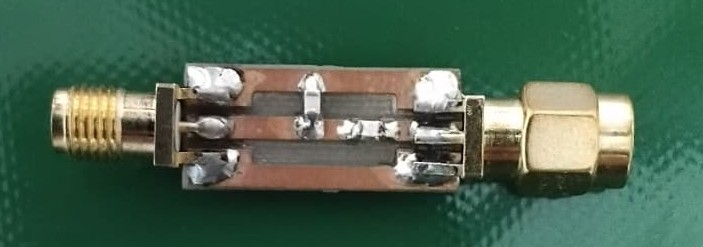
\includegraphics[width=0.6\linewidth]{Imagens/PCB_real.jpg}}
        \caption{Manufactured PCB photograph}
        \label{cap3:sec7:fig3:c}
    \end{subfigure}
    \caption{PCB layout model in QucsStudio , design in EasyEDA, and photograph of the manufactured.}
    \label{cap3:sec7:fig3}
\end{figure}


\section{Estimated Component Costs}
Table~\ref{tab:component_prices} summarises the average prices of the main components used in this project, both in Portugal and in the Asian market. Although these values are only indicative, they provide a realistic estimate of the typical costs involved. The total amount is modest, underscoring the low-cost nature of the design. When compared with the commercial equipment discussed in Chapter \ref{cap2:State_Of_The_Art}, the cost of this project represents only a small fraction.


\newpage

\begin{table}[H]
\centering
\caption{Estimated cost of components used in the project.}
\label{tab:component_prices}
\begin{tabular}{|l|c|c|}
\hline
\textbf{Component} & \textbf{Portugal} & \textbf{Asian Market} \\ \hline
Arduino UNO & \euro\;29.50 & \euro\;3.80 \\ \hline
Dual Bipolar Stepper Motor Shield for Arduino (DRV8825) & \euro\;34.50 & \euro\;6.80 \\ \hline
2 Hall-effect sensors & \euro\;5.38 & \euro\;0.44 \\ \hline
2 NEMA17 stepper motors & \euro\;24.00 & \euro\;16.54 \\ \hline
1.5 m GT2 timing belt (6 mm) & \euro\;3.60 & \euro\;2.58 \\ \hline
20-teeth pulley for NEMA17 stepper motor & \euro\;3.70 & \euro\;2.56 \\ \hline
Power supply 230V$\sim$12V - 2A & \euro\;4.97 & \euro\;4.68 \\ \hline
2 m fibreglass tube, 18 mm (12 mm inner) & \euro\;52.28 & \euro\;22.70 \\ \hline
1 Kg PLA filament (1.5 mm) & \euro\;15.49 & \euro\;7.00 \\ \hline
Electronic wires for connection & \euro\;15.52 & \euro\;6.32 \\ \hline
RF sensor detector & \euro\;20.70 & \euro\;8.58 \\ \hline
868 MHz band-pass filter & \euro\;14.95 & \euro\;5.57 \\ \hline
2 m copper rod (3 mm or 4 mm) & \euro\;7.60 & \euro\;4.25 \\ \hline
FR-4 copper-clad laminate (20X30 cm) & \euro\;6.96 & \euro\;5.24 \\ \hline
4 RF connector SMD (Male and Female) & \euro\;29.92 & \euro\;4.92 \\ \hline
Capacitor and Inductor SMD 0805  & \euro\;0.90 & \euro\;0.50 \\ \hline
Screws and Threads & \euro\;8.46 & \euro\;3.27 \\ \hline
2 nylon bearings & \euro\;3.86 & \euro\;1.35 \\ \hline
2 standard bearings & \euro3.94 & \euro\;3.15 \\ \hline
4 ball bearing with collar  & \euro\;15.25 & \euro\;3.85 \\ \hline
3 bases (wood or equivalent), Ø 30 cm & \euro\;4.80 & \euro\;8.10 \\ \hline
\textbf{TOTAL} & \textbf{\euro\;306.28} & \textbf{\euro\;122.20} \\ \hline
\end{tabular}
\end{table}

\indent The subsequent chapter presents the experimental results obtained and discusses their impact, considering the materials and methods described previously.
%-----------------------------------------------------------------------------------------------------
\chapter{Results}
\label{cap:resultados_obtidos}
%-----------------------------------------------------------------------------------------------------

%-----------------------------------------------------------------------------------------------------
\section{Introduction}
%-----------------------------------------------------------------------------------------------------

This chapter presents the experimental results obtained from the characterisation of the antennas, the balun, the impedance matching PCB, and the 868~MHz band-pass filter, as well as from the complete antenna radiation pattern measurement system. The band-pass filter, based on SAW (Surface Acoustic Wave) technology, was included in the setup to suppress out-of-band noise and interference. The initial objective of these measurements was to validate the performance of the antennas individually, both the transmitting and receiving antennas, which exhibit very similar, though not identical, behaviour due to slight manufacturing differences.

Measurements were carried out mainly with a VNA, supported by an RF signal generator and, in some cases, with a Spectrum Analyzer (SA). For each element, $S_{11}$ and, where relevant, $S_{21}$ parameters were measured to evaluate impedance matching, signal integrity, and the suppression of undesired common modes. All measurements are presented together with their corresponding plots for clarity.

Among the different characterisations, the antenna radiation pattern was of particular interest, as it directly reflects the Yagi-Uda design and provides a key indicator of the overall system performance.


%-----------------------------------------------------------------------------------------------------
\section{Measurement Setup}
%-----------------------------------------------------------------------------------------------------

The objective of this measurement setup was to obtain the horizontal (azimuth) radiation pattern of the antenna under test and to validate the far-field measurement conditions.

The transmitting and receiving antennas were initially characterised using a NanoVNA at 868~MHz. After that, the band-pass filter was also verified for compliance with the operating frequency requirements.

For the far-field radiation pattern measurement, the minimum far-field distance was calculated using (\ref{eq:farfield_distance}):

\begin{equation}
    d = \frac{2R^{2}}{\lambda}
    \label{eq:farfield_distance}
\end{equation}

where $R$ is the largest dimension of the antenna, equivalent to the boom length in the case of the Yagi-Uda, and $\lambda$ is the wavelength. For $R = 0.3~\text{m}$ and $\lambda \approx 0.345~\text{m}$, $d \approx 0.52~\text{m}$. To ensure far-field conditions, the antennas were spaced $D = 2.5~\text{m}$ apart.


The transmitting antenna was a Yagi-Uda with a gain of approximately $10~\text{dB}$, with a maximum input power of $0.5~\text{mW}$ ($-3~\text{dBm}$) to comply with an EIRP (Effective Isotropic Radiated Power) of 5~mW. Using the Friis equation (\ref{eq:friis}) \cite{Friis1946}, which relates transmitted and received power in free space, the expected received power can be calculated. Assuming an isotropic receiving antenna, the result is:

\begin{align}
    P_{\mathrm{rx}} &= P_{\mathrm{tx}} + G_{\mathrm{tx}} + G_{\mathrm{rx}} - 20 \log_{10} \left( \frac{4 \pi D}{\lambda} \right) \label{eq:friis} \\
    P_{\mathrm{rx}} &= -3 + 10 + 0 - 20 \log_{10} \left( \frac{4 \pi \times 2.5}{0.3456} \right)  \\
    P_{\mathrm{rx}} &\approx -32~\text{dBm (in free-space conditions).} 
\end{align}

Considering, however, that the receiving antenna is also a Yagi-Uda with a gain of about $10~\text{dB}$, the expected received power rises to approximately $-22$~dBm, which is in line with the measured results discussed later (between $-22$ and $-18$~dBm).

Measurements were performed outdoors to minimise multipath effects, with both antennas mounted at least 1~m above ground on fibreglass supports to reduce ground reflections. The receiving antenna was rotated in azimuth in $5^{\circ}$ steps, while the transmitting antenna remained fixed.

The signal power was measured using an AD8313 detector, calibrated before the measurements began. The calibration data were obtained from a reference measurement setup, as shown in Figure \ref{cap4:sec2:fig1}, and the relationship between the input signal power and the output voltage of the integrated circuit was determined using the weighted least squares method, as shown in:

\begin{equation}
    V_\text{out} = 0.0185 \cdot P_\text{in} + 1.8621
\end{equation}

yielding a sensitivity of approximately 19~mV/dBm, close to the 18~mV/dBm from the datasheet.

\begin{figure}[H]
    \centering
    % Left: larger image
    \begin{subfigure}{0.378\textwidth}
        \centering
        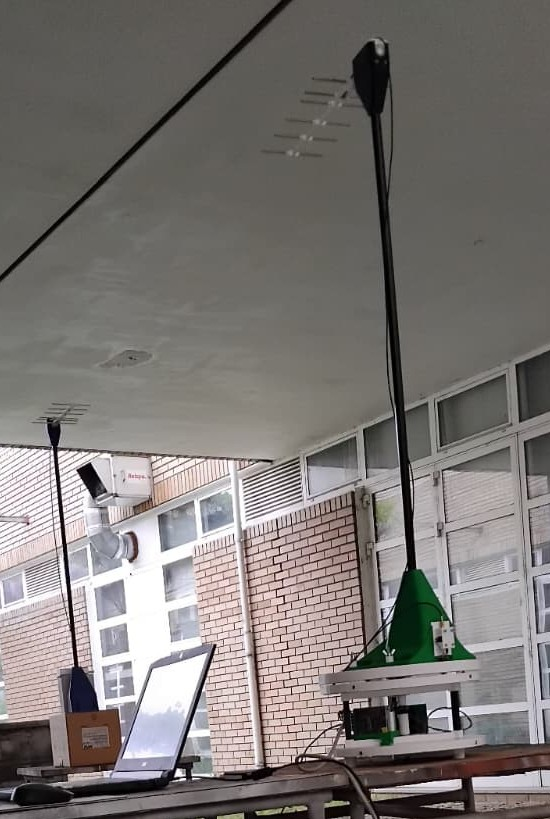
\includegraphics[width=\textwidth]{Imagens/setup1.jpg}
        \caption{Setup rear view}
        \label{fig:setup:a}
    \end{subfigure}
    \hspace{0.5mm}
    % Right: two smaller images stacked
    \begin{minipage}{0.6\textwidth}
        \begin{subfigure}{\textwidth}
            \centering
            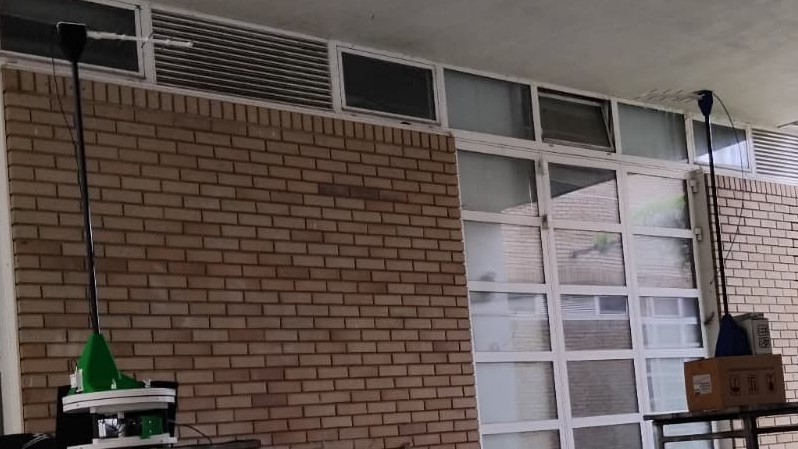
\includegraphics[width=0.76\textwidth]{Imagens/setup2.jpg}
            \caption{Setup side view(closer)}
            \label{fig:setup:b}
        \end{subfigure}
        \vskip 1mm
        \begin{subfigure}{\textwidth}
            \centering
            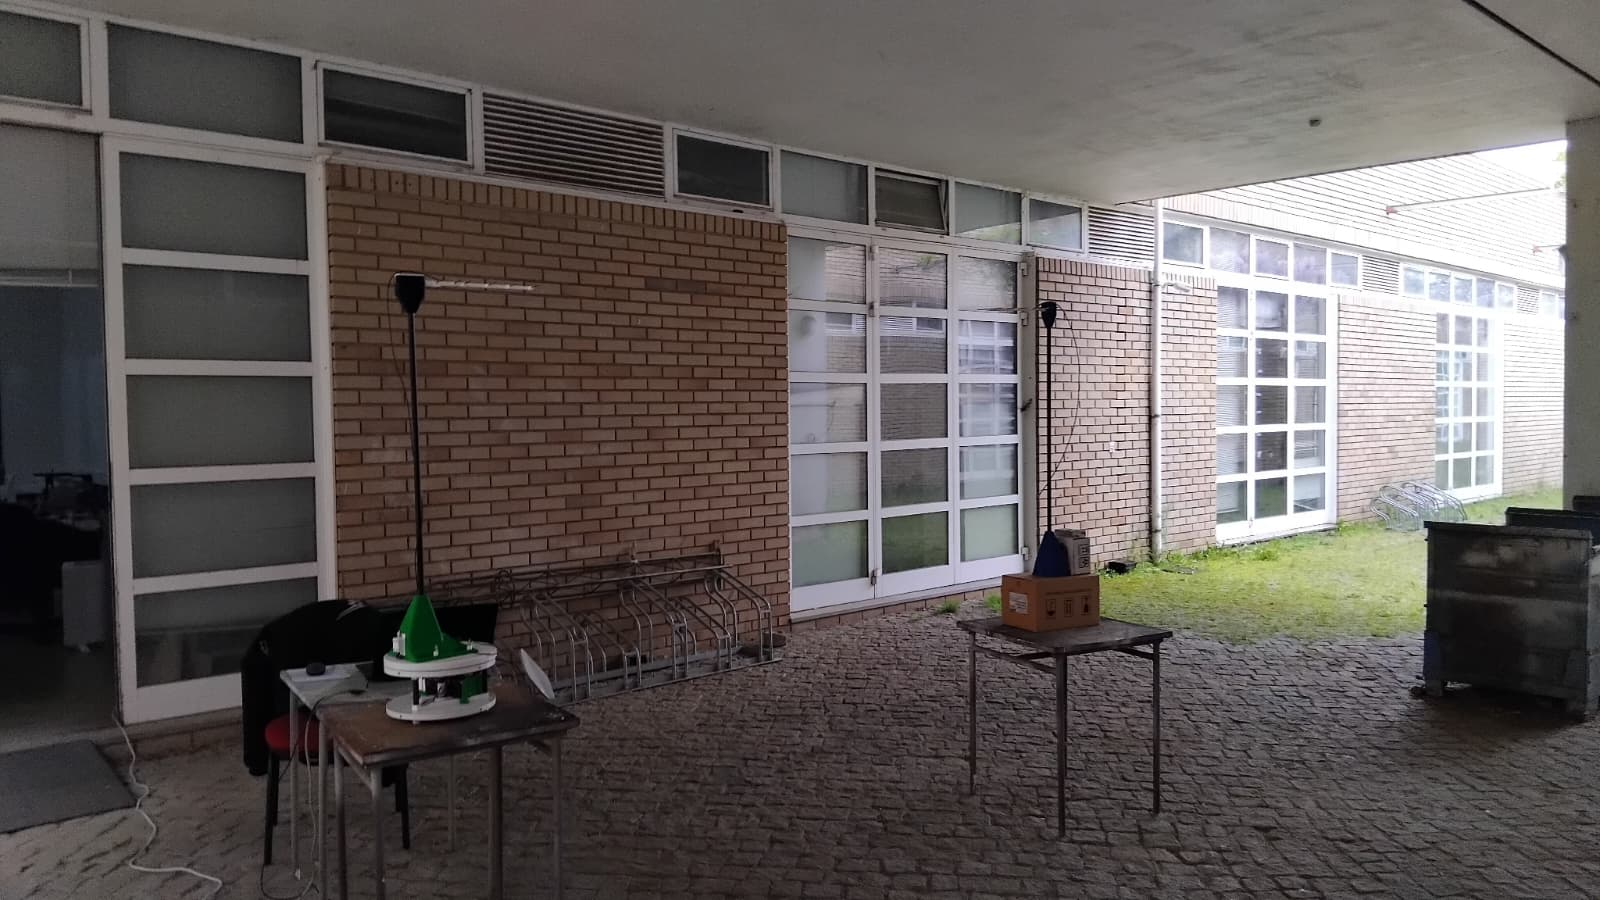
\includegraphics[width=0.76\textwidth]{Imagens/setup3.jpg}
            \caption{Setup side view}
            \label{fig:setup:c}
        \end{subfigure}
    \end{minipage}
    \caption{Experimental setup for transmitting and receiving antennas, showing rear and side perspectives.}
    \label{cap4:sec2:fig1}
\end{figure}


%-----------------------------------------------------------------------------------------------------
\section{Characterisation of Components}
%-----------------------------------------------------------------------------------------------------

The characterisation of the components was performed using the NanoVNAsaver\footnote{NanoVNAsaver is an open-source software that reads data from the NanoVNA and displays it on a computer.} and, where applicable, a TinySA (spectrum analyzer). Measurements focused on the relevant scattering parameters (S-parameters) of each component.

In this work, only the most relevant S-parameters are considered, namely $S_{11}$ and $S_{21}$. However, the others parameters are:

\begin{itemize}
    \item $S_{11}$: reflection coefficient at port 1, indicating the matching of the input impedance.

    \item $S_{21}$: forward transmission from port 1 to port 2, representing insertion loss or gain.

    \item $S_{22}$: reflection coefficient at port 2, indicating the matching of the output impedance.
    
    \item $S_{12}$: reverse transmission from port 2 to port 1, representing isolation or reverse gain.


\end{itemize}

In addition, to complement the analysis of impedance matching, the Voltage Standing Wave Ratio (VSWR) was also considered. VSWR is directly related to $S_{11}$ and indicates how effectively power is transferred from the source to the load, with values close to 1 indicating good matching, and values above 2 are generally considered poor.


%-----------------------------------------------------------------------------------------------------
\subsection{868~MHz Band-Pass Filter}
%-----------------------------------------------------------------------------------------------------

The measured response confirms that the filter effectively attenuates out-of-band signals and reduce unwanted noise, thereby improving the selectivity of the measurement system. Figure~\ref{cap4:sec3:subsec2:fig1} shows the measured $S_{21}$ parameter, representing the insertion loss.

\begin{figure}[H]
    \centering
    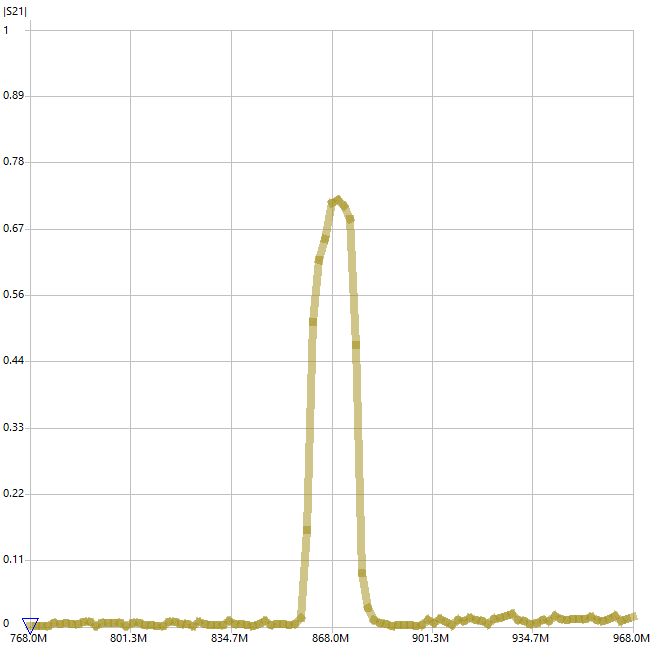
\includegraphics[width=0.72\textwidth]{Imagens/filtro/fig1.png}
    \label{cap4:sec3:subsec2:fig1:a}
    \caption{$S_{21}$ of the 868~MHz band-pass filter showing insertion loss and passband characteristics.}
    \label{cap4:sec3:subsec2:fig1}
\end{figure}

At the centre frequency of 868~MHz, the insertion loss is approximately 3~dB, which is consistent with the manufacturer’s specifications. The bandwidth extends from about 860~MHz to 880~MHz, typical of commercial ISM band-pass filters. This response ensures that the antenna operates effectively within the intended frequency range while suppressing frequencies outside it.


The measured attenuation will be taken into account in the subsequent radiation pattern measurements, as it directly affects the received signal strength.


%-----------------------------------------------------------------------------------------------------
\subsection{Balun}
%-----------------------------------------------------------------------------------------------------

The transmission coefficient $S_{21}$ of the balun was measured using a VNA to evaluate its performance in converting between balanced and unbalanced signals. The results, shown in Figure~\ref{cap4:sec3:subsec3:fig1}, indicate a differential mode insertion loss of approximately $-0.58$~dB at 868~MHz and a common mode attenuation greater than $-47$~dB at the same frequency. Additional measurements confirmed good impedance matching at both ports.
\vspace{-1em}
\begin{figure}[!ht]
    \centering
    \begin{subfigure}[b]{0.48\textwidth}
        \centering
        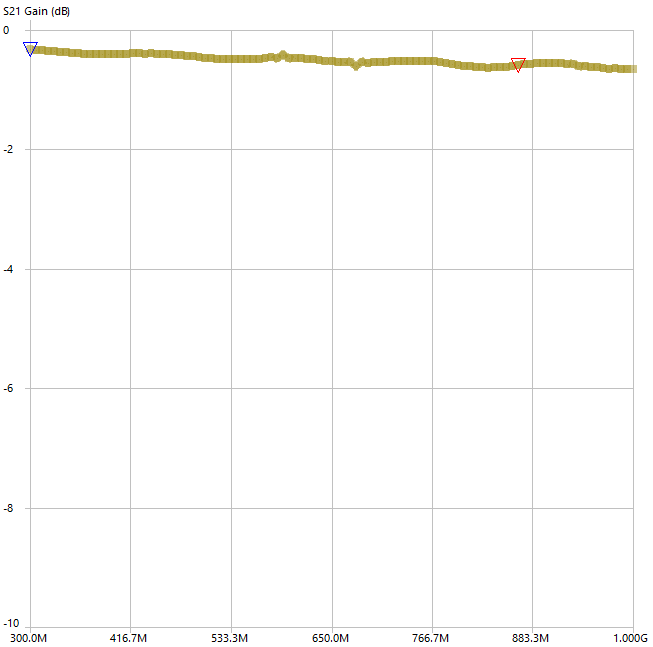
\includegraphics[width=\textwidth]{Imagens/balun_caract/insertion_loss.png}
        \caption{Differential mode: insertion loss of $\approx -0,58$~dB at 868~MHz.}
        \label{cap4:sec3:subsec3:fig1:a}
    \end{subfigure}
    \hfill
    \begin{subfigure}[b]{0.48\textwidth}
        \centering
        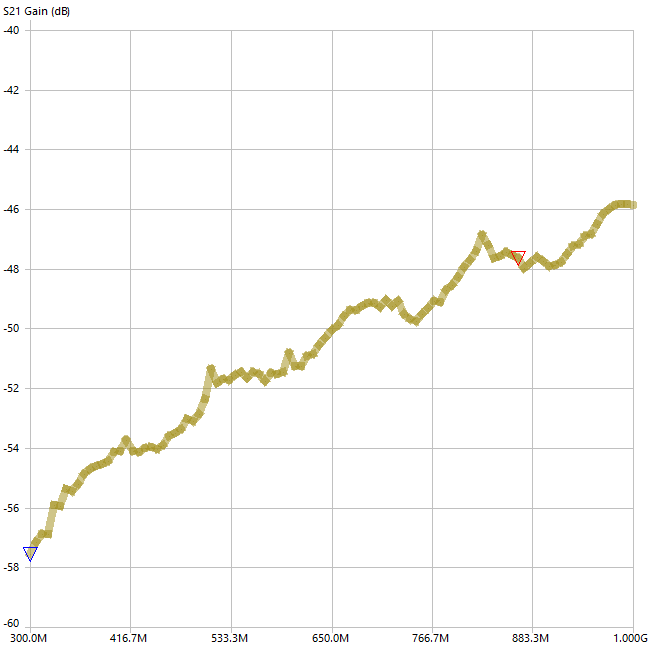
\includegraphics[width=\textwidth]{Imagens/balun_caract/insertion_loss2.png}
        \caption{Common mode: attenuation greater than $-47$ dB at 868 MHz.}
        \label{cap4:sec3:subsec3:fig1:b}
    \end{subfigure}
    \caption{Experimental S21 results for the air choke balun using VNA in differential and common modes.}
    \label{cap4:sec3:subsec3:fig1}
\end{figure}


%-----------------------------------------------------------------------------------------------------
\subsection{PCB for Impedance Matching}
%-----------------------------------------------------------------------------------------------------

The S-parameters of the PCB confirm the effectiveness of the impedance matching network, as shown in Figure \ref{cap4:sec3:subsec4:fig1}. 
At the 868~MHz frequency, the reflection coefficient at the input port is 
$S_{11} \approx -20.3$~dB. 
This translates to a VSWR of approximately $1.213$, close to the ideal value of~1. 
The input impedance measured at this frequency is $43.1 - j5.76~\Omega$, close to the nominal $50~\Omega$ reference. 
Such results demonstrate that the reflected power is reduced to below $1\%$, confirming an excellent matching performance. Other parameters were omitted, as they provided no further insight into the matching performance.

\begin{figure}[H]
    \centering
    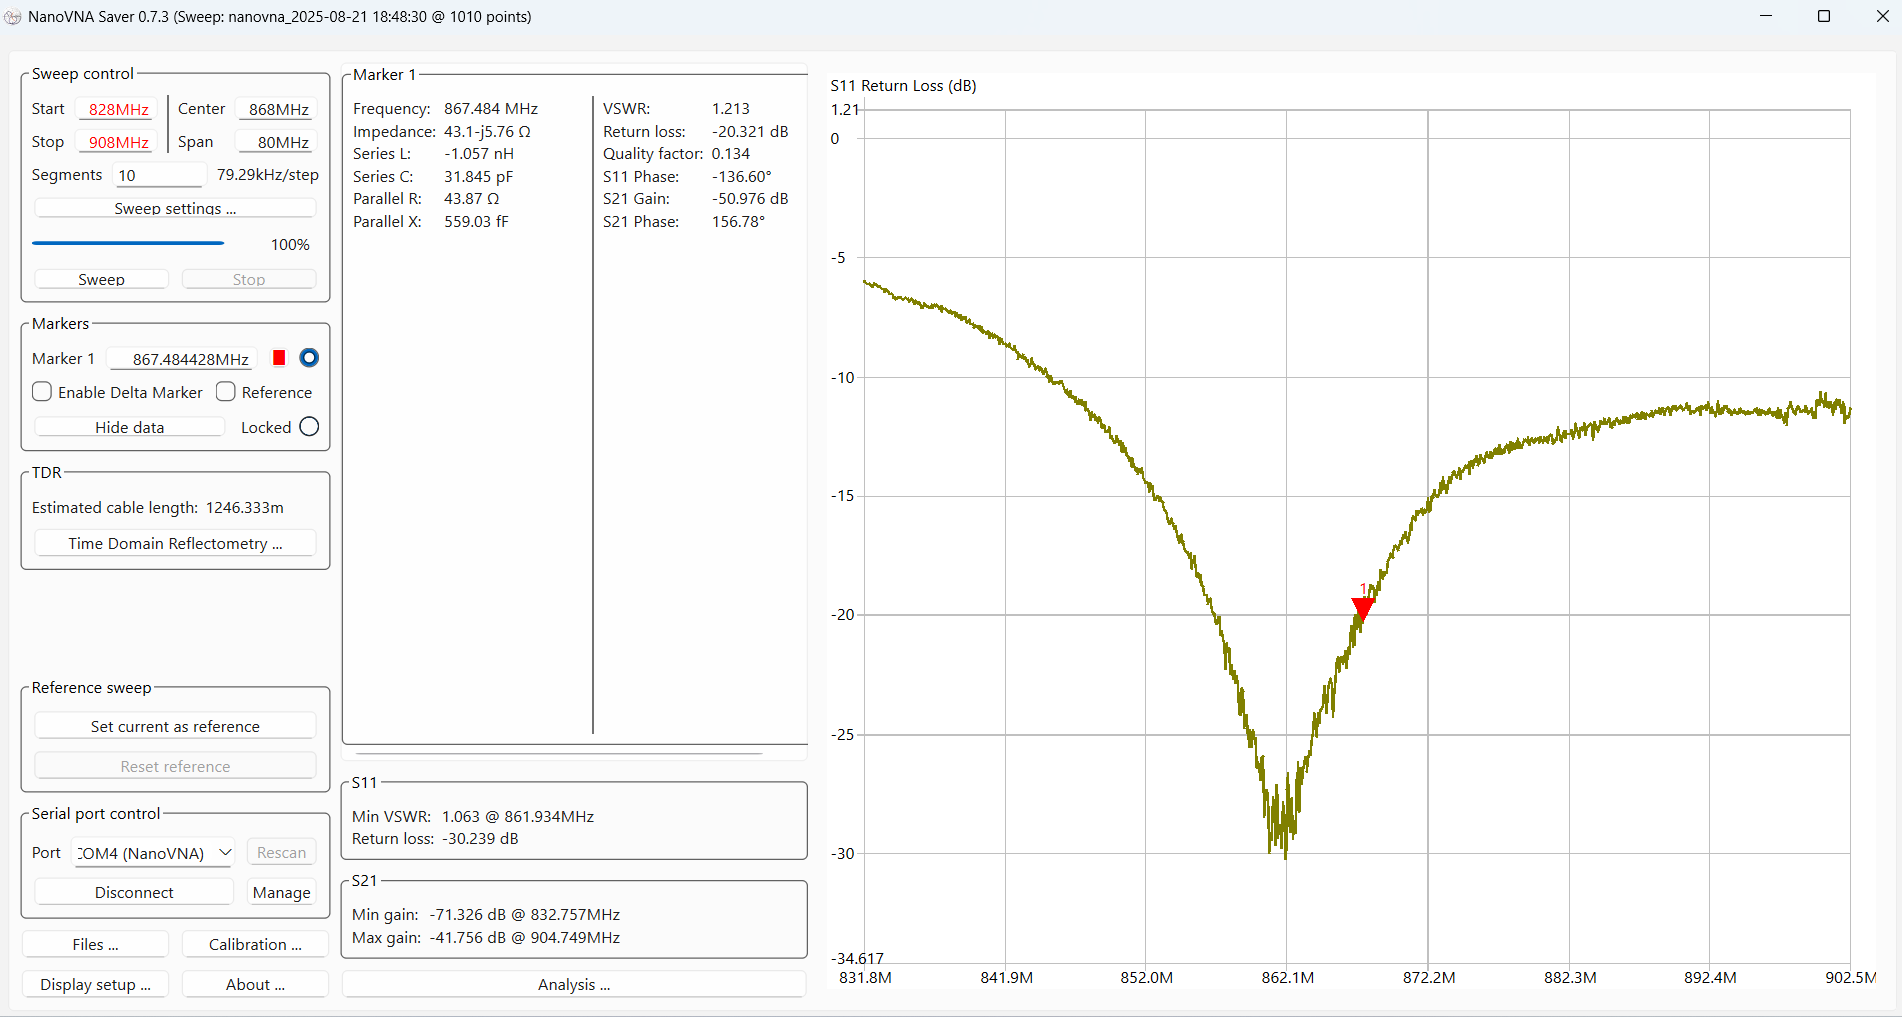
\includegraphics[width=0.98\textwidth]{Imagens/carcaterização do PCB/S11 e S21 v4 mais um L de 3.3 em serie complta Tx.png}
    \caption{$S_{11}$ graph and VSWR of the PCB used for impedance matching}
    \label{cap4:sec3:subsec4:fig1}
\end{figure}

%-----------------------------------------------------------------------------------------------------
\subsection{Reflection Coefficient and Matching Performance}
%-----------------------------------------------------------------------------------------------------

Matching improvement was quantified by evaluating the reflection coefficient ($\Gamma$) and reflected power. 
The relationships between return loss, reflection coefficient, and reflected power are well-established in microwave engineering \cite{pozar2011}.

The return loss (RL) is related to the voltage reflection coefficient $\Gamma$ as:
\begin{equation}
\label{eq:RL}
RL = -10 \log_{10}\left|\frac{P_{\text{refl}}}{P_{\text{inc}}}\right|
   = -20 \log_{10}\left|\frac{V_{\text{refl}}}{V_{\text{inc}}}\right|
   = -20 \log_{10}|\Gamma|
\end{equation}

Equivalently, the S-parameter $S_{11}$ is related to the reflection coefficient as:
\begin{equation}
\label{eq:S11}
S_{11} = -RL = 20 \log_{10} |\Gamma| \xrightarrow{} |\Gamma| = 10^{-\tfrac{RL}{20}}
\end{equation}

Finally, the fraction of reflected power can be expressed as:
\begin{equation}
\label{eq:Preflected}
P_{\text{refl}} = |\Gamma|^2
\end{equation}

These equations are directly related: the return loss determines the magnitude of the reflection coefficient, which in turn gives the fraction of reflected power. This allows an intuitive interpretation of matching performance in terms of the percentage of incident power that is reflected back. In practical terms, the complement $1-|\Gamma|^2$ corresponds to the fraction of power actually delivered to the load, providing a direct link between return loss and system efficiency. For instance, a return loss of 10~dB corresponds to about 10\% reflected power, while 20~dB corresponds to only 1\%, values that are typically regarded as acceptable or good in RF design.


\subsection*{Before Matching}
For a measured return loss of $RL \approx 11$~dB:
\begin{align}
|\Gamma| &= 10^{-\tfrac{RL}{20}} \label{eq:Gamma}\\
|\Gamma| &= 10^{-\tfrac{11}{20}} \approx 0.2818, \label{eq:GammaBefore}\\
P_{\text{refl}} &= (0.2818)^2 \approx 0.079 \ (\text{or } 7.9\%)
\end{align}

\subsection*{After Matching}
With the return loss improved to $RL \approx 20.3$~dB:
\begin{align}
|\Gamma| &= 10^{-\tfrac{RL}{20}} \\
|\Gamma| &= 10^{-\tfrac{20.3}{20}} \approx 0.096, \label{eq:GammaAfter}\\
P_{\text{refl}} &= (0.096)^2 \approx 0.0092 \ (\text{or } 0.92\%)
\end{align}

These results show that the reflected power was reduced from approximately 8\% to less than 1\% of the incident power, 
which corresponds to a significant improvement in power transfer efficiency. This analysis confirms that, despite the impedance of $43.1-j5.76 \ \Omega$, the antenna system exhibits significantly improved matching compared to the initial condition.
%-----------------------------------------------------------------------------------------------------


%-----------------------------------------------------------------------------------------------------
\section{Radiation Pattern Measurement}
%-----------------------------------------------------------------------------------------------------

This section presents the measurement of the azimuth radiation pattern of the antenna under test. The objective is to assess the real-world performance of the antenna and compare it with the ideal model obtained from simulations in CST Studio Suite. At the end of this section, the 3D pattern is also displayed, and although it shows only the azimuth axis, the DUT could be evaluated on a second axis perpendicular to the first.

It should be noted that the simulated model assumes a vacuum environment without reflections, while the measurements are conducted under outdoor conditions with potential multipath effects. Despite these differences, the basic radiation characteristics of the antenna are expected to align with the simulation, providing a reference for subsequent evaluations with additional components such as the band-pass filter, balun, and impedance matching network.

%-----------------------------------------------------------------------------------------------------
\subsection{Antenna Only}
%-----------------------------------------------------------------------------------------------------

The measured radiation pattern shows the main lobe and side lobes of the antenna, which can be compared to the ideal simulated model. Minor deviations are expected due to environmental factors. 

As shown in Figure~\ref{cap4:sec4:subsec1:fig1}, both the measured and simulated radiation patterns exhibit a main lobe centred at 90$^{\circ}$, confirming that the system is able to determine the direction of maximum radiation. The measured half-power beamwidth is 49.1$^{\circ}$, which is in close agreement with the simulated value of 47.7$^{\circ}$. The front-to-back ratio was measured at 17.0~dB, compared to 16.3~dB obtained in simulation (not shown in the figure). These results indicate that the proposed setup is capable of reproducing the main features of the radiation pattern, including the main lobe and the secondary lobes.

In spite of this, this first antenna radiation pattern measurement provides the main feedback to improve the results.

\begin{figure}[H]
     \centering
     \begin{subfigure}{0.61\textwidth}
         \centering
         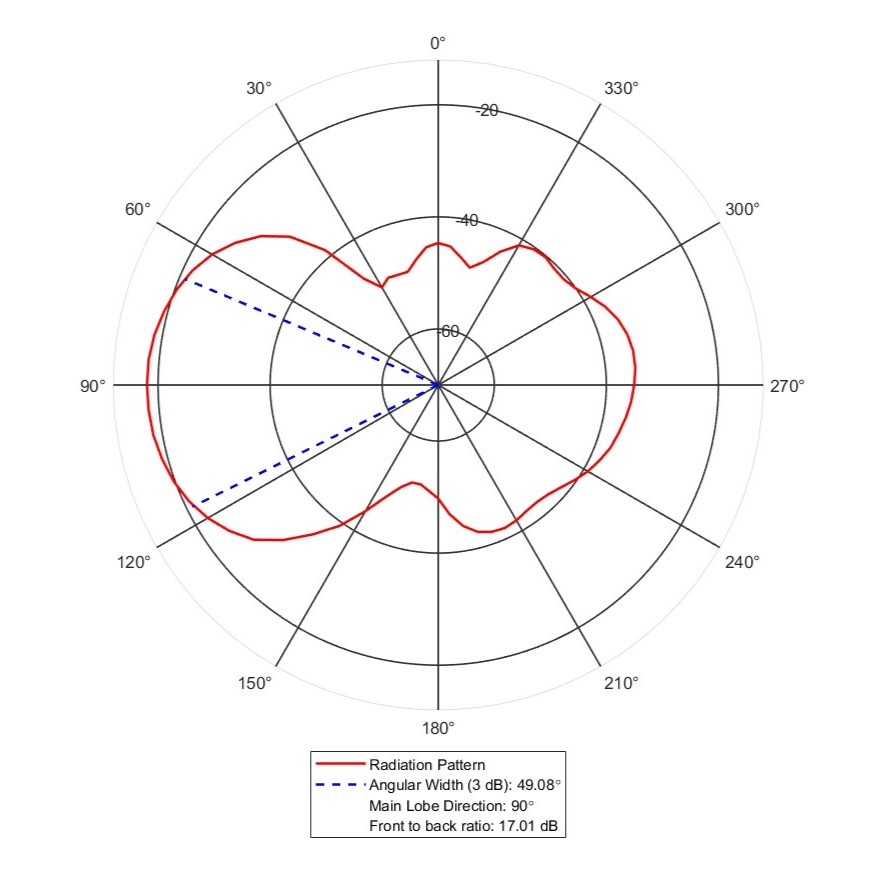
\includegraphics[width=\textwidth]{Imagens/Real_data_acquired.jpg}
         \caption{Real data acquired}
         \label{cap4:sec4:subsec1:fig1:a}
     \end{subfigure}
     \hspace{1mm}
     \begin{subfigure}{0.78\textwidth}
         \centering
         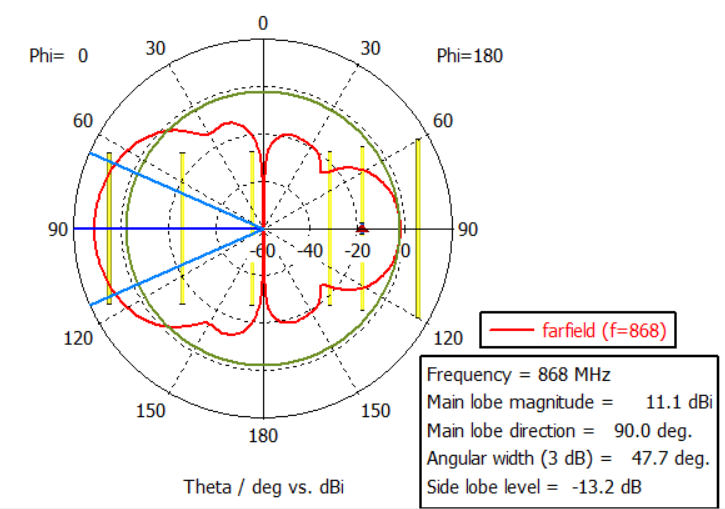
\includegraphics[width=\textwidth]{Imagens/simulationv3.png}
         \caption{Simulation of the radiation pattern}
         \label{cap4:sec4:subsec1:fig1:b}
     \end{subfigure}
        \caption{Comparison of real and simulated radiation pattern.}
        \label{cap4:sec4:subsec1:fig1}
\end{figure}

%-----------------------------------------------------------------------------------------------------
\subsection{Antenna with Band-Pass Filter}
%-----------------------------------------------------------------------------------------------------

The inclusion of the band-pass filter introduces a small insertion loss and minor modifications to the radiation pattern, which are visible when comparing the measurement to the simulation, as illustrated in Figure \ref{cap4:sec4:subsec2:fig1}

\begin{figure}[H]
     \centering
     \begin{subfigure}{0.45\textwidth}
         \centering
         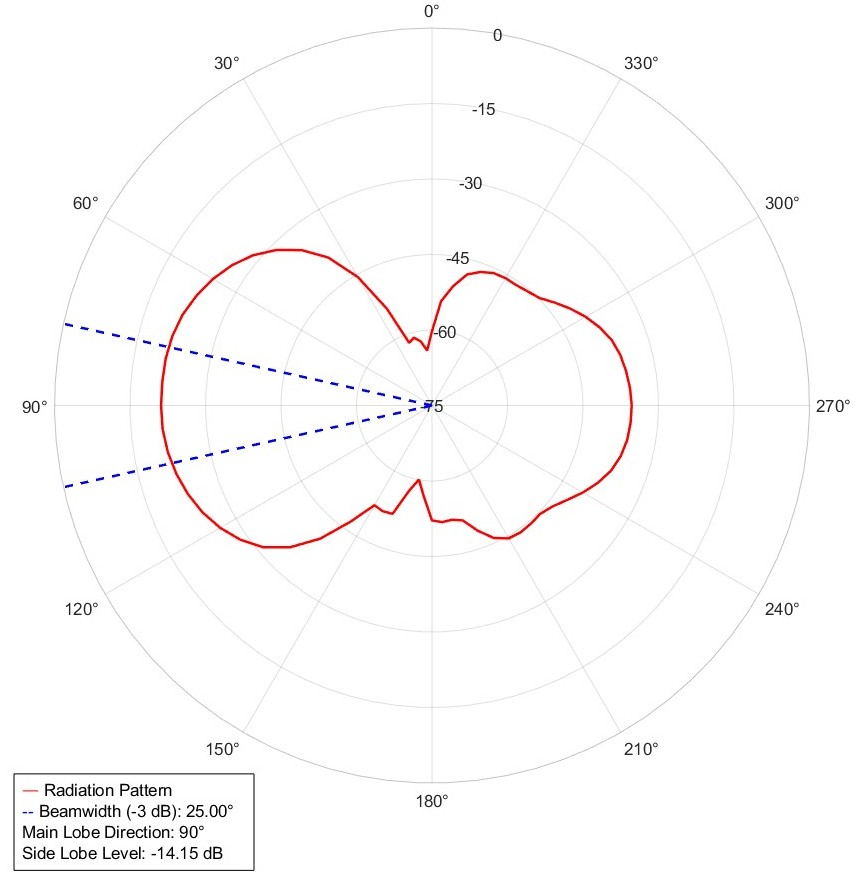
\includegraphics[width=\textwidth]{Imagens/Real_data_with_filter.jpg}
         \caption{Real data acquired with 868 MHz band-pass filter}
         \label{cap4:sec4:subsec2:fig1:a}
     \end{subfigure}
     \hspace{1mm}
     \begin{subfigure}{0.69\textwidth}
         \centering
         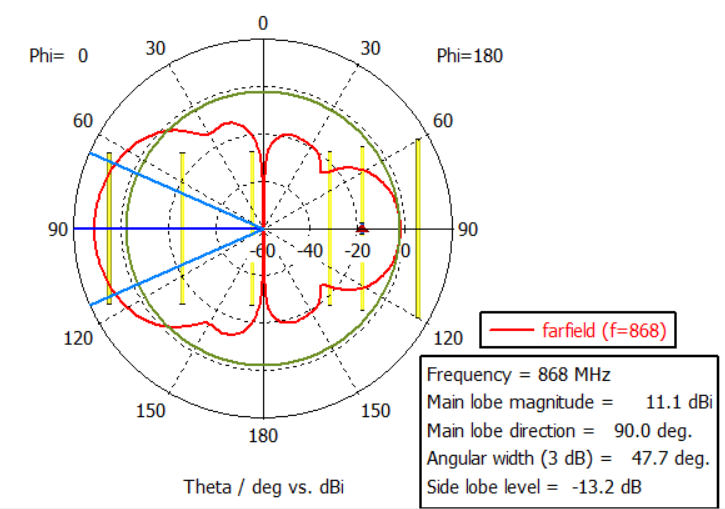
\includegraphics[width=\textwidth]{Imagens/simulationv3.png}
         \caption{Simulation of the radiation pattern on CST Studio Suite}
         \label{cap4:sec4:subsec2:fig1:b}
     \end{subfigure}
        \caption{Comparison of real and simulated radiation pattern. Antenna with band-pass filter.}
        \label{cap4:sec4:subsec2:fig1}
\end{figure}


%-----------------------------------------------------------------------------------------------------
\subsection{Antenna with Band-Pass Filter and Balun}
%-----------------------------------------------------------------------------------------------------

Adding the balun modifies the current distribution in the antenna, slightly affecting the shape of the radiation pattern compared to the previous configuration, as it is possible to visualise in Figure~\ref{cap4:sec4:subsec3:fig1}.

\begin{figure}[H]
     \centering
     \begin{subfigure}{0.45\textwidth}
         \centering
         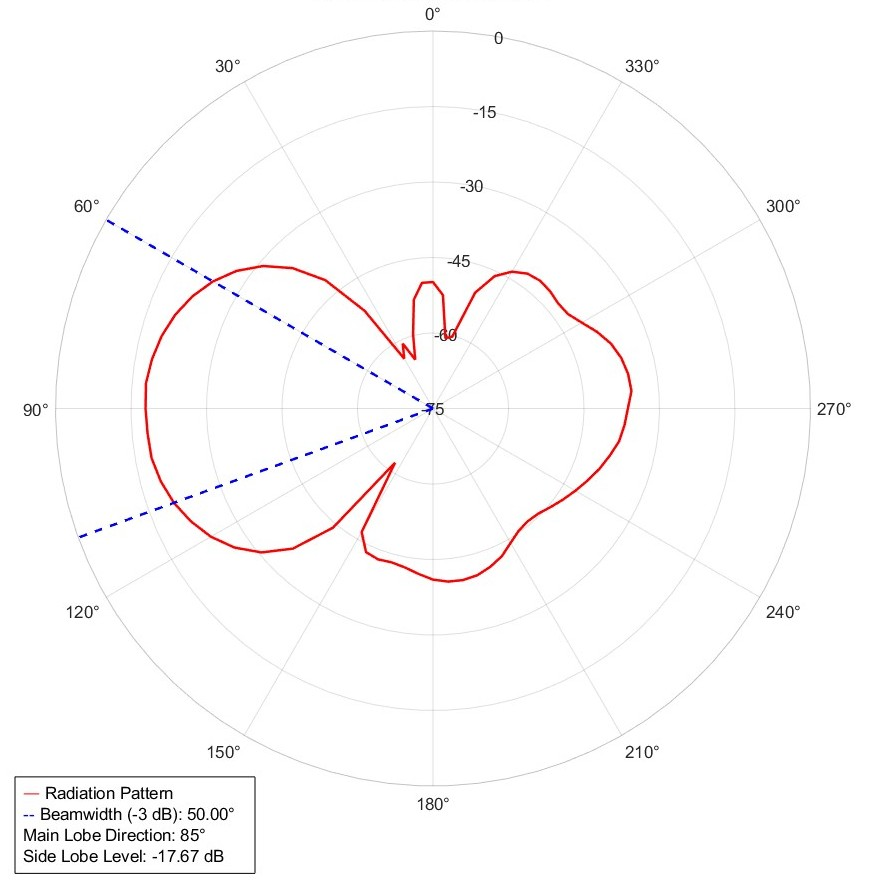
\includegraphics[width=\textwidth]{Imagens/media_real.jpg}
         \caption{Real data acquired with 868 MHz band-pass filter and balun.}
         \label{cap4:sec4:subsec3:fig1:a}
     \end{subfigure}
     \hspace{1mm}
     \begin{subfigure}{0.69\textwidth}
         \centering
         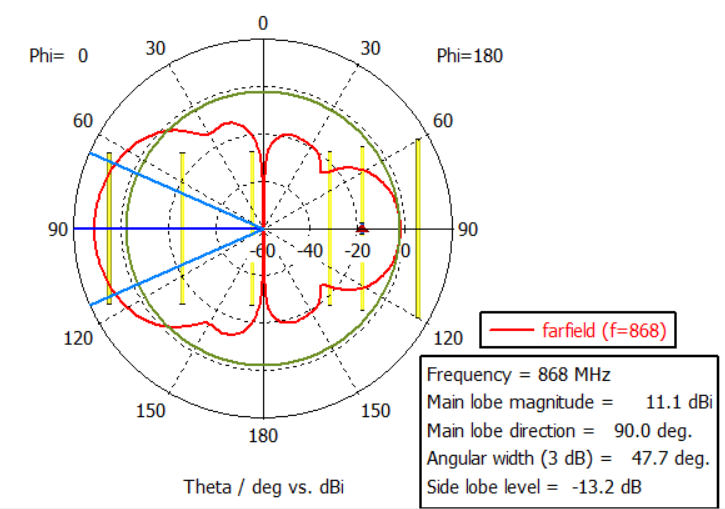
\includegraphics[width=\textwidth]{Imagens/simulationv3.png}
         \caption{Simulation of the radiation pattern on CST Studio Suite}
         \label{cap4:sec4:subsec3:fig1:b}
     \end{subfigure}
        \caption{Comparison of real and simulated radiation pattern. Antenna with band-pass filter and balun.}
        \label{cap4:sec4:subsec3:fig1}
\end{figure}

The inclusion of the band-pass filter introduces a small insertion loss ($\approx$ 3 dB) without significantly altering the main lobe of the radiation pattern.




%-----------------------------------------------------------------------------------------------------
\subsection{Antenna with Band-Pass Filter, Balun, and Impedance Matching Network}
%-----------------------------------------------------------------------------------------------------




The full configuration, including the impedance matching network, provides the most realistic representation of the final system, as can be seen in Figure \ref{cap4:sec4:subsec4:fig1}. Interestingly, the inclusion of the additional components not only preserved the main radiation characteristics but also brought the measured pattern into closer agreement with the theoretical model, showed in Figure \ref{cap4:sec4:subsec4:fig2}. Minor deviations remain, primarily due to practical insertion losses and environmental reflections.

\begin{figure}[H]
    \centering
    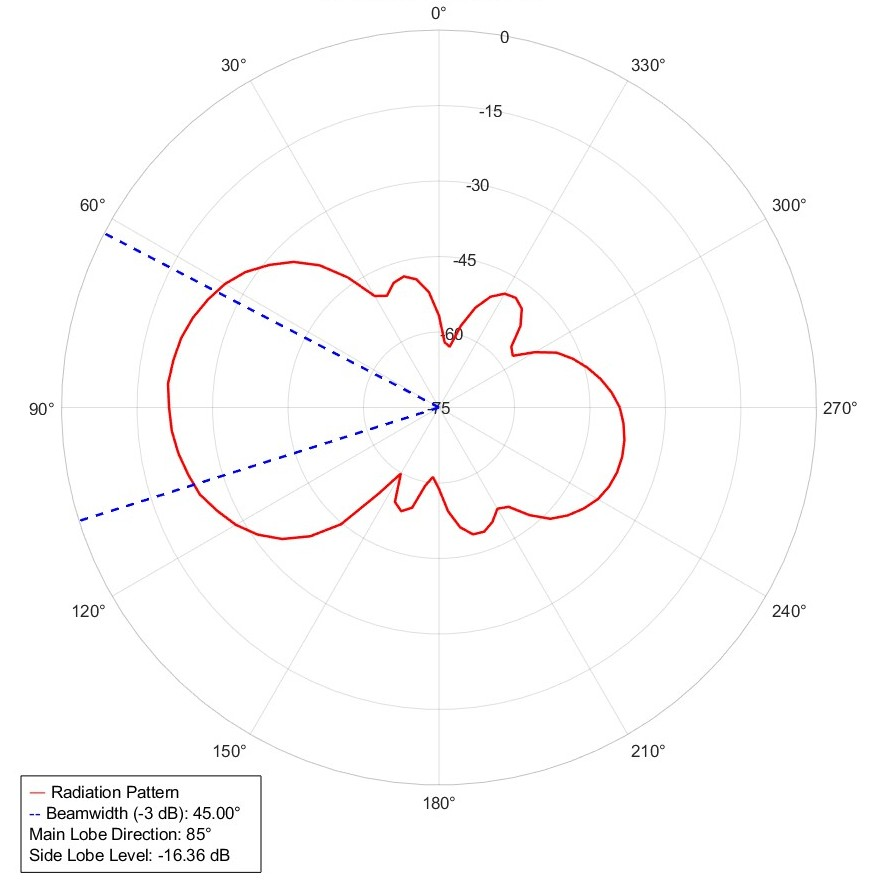
\includegraphics[width=0.65\textwidth]{Imagens/medianew.jpg}
    \caption{Measured data with filter, balun and impedance matching.}
    \label{cap4:sec4:subsec4:fig1}
\end{figure}

\begin{figure}[H]
    \centering
    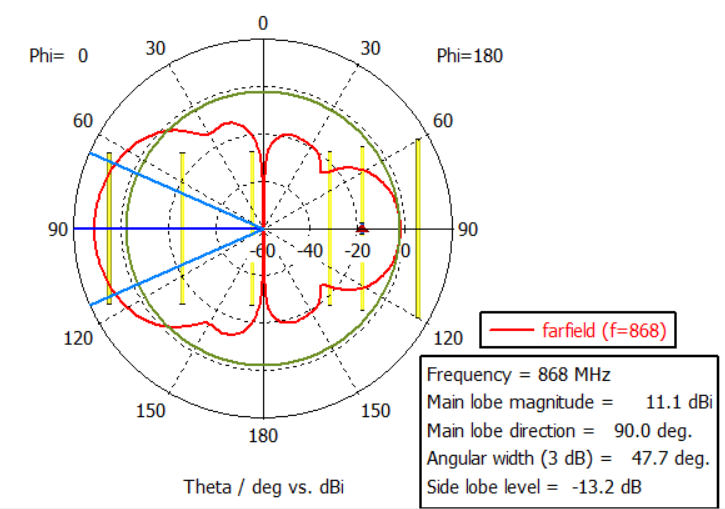
\includegraphics[width=0.95\textwidth]{Imagens/simulationv3.png}
    \caption{Simulated radiation pattern outcome from CST Studio Suite.}
    \label{cap4:sec4:subsec4:fig2}
\end{figure}


\subsubsection{3D Radiation Pattern}

Although two-dimensional radiation patterns are useful for quickly assessing antenna performance, they provide a partial view of how the radiated power is distributed in space. A full three-dimensional radiation pattern offers a more complete characterisation, allowing to see asymmetries and distortions that might not be evident in 2D slices. For this reason, a 3D measurement was carried out to complement the 2D analyses.

The three-dimensional radiation pattern of the complete antenna system was also measured and compared with the simulated model obtained in CST Studio Suite, as shown in Figure \ref{cap4:sec4:subsec4:fig3} and Figure \ref{cap4:sec4:subsec4:fig4}. Despite some distortions observed in the experimental result, a general agreement with the simulation can be identified. This confirms that the proposed measurement system is able to operate with two degrees of freedom and to characterise the radiation pattern in three dimensions.

\begin{figure}[H]
    \centering
    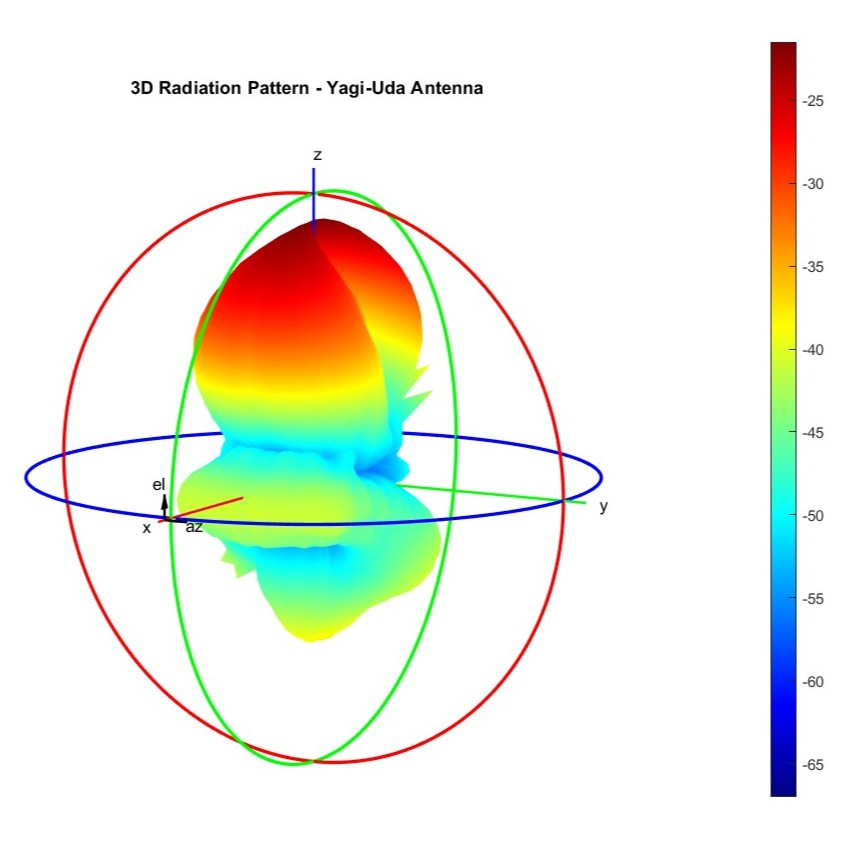
\includegraphics[width=0.7\textwidth]{Imagens/new_3d.jpg}
    \caption{Measured 3D radiation pattern.}
    \label{cap4:sec4:subsec4:fig3}
\end{figure}

\begin{figure}[H]
    \centering
    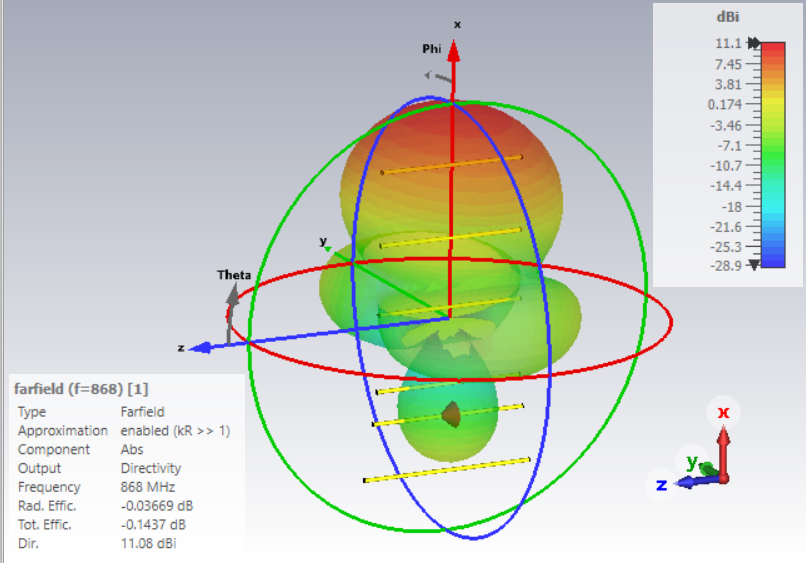
\includegraphics[width=0.7\textwidth]{Imagens/3Dsimulation.png}
    \caption{Simulated 3D radiation pattern from CST Studio Suite.}
    \label{cap4:sec4:subsec4:fig4}
\end{figure}


%-----------------------------------------------------------------------------------------------------
\section{Discussion of Results}
%-----------------------------------------------------------------------------------------------------

This section will be developed to provide both a concise overview of the obtained measurements and a summary of the main observations. The individual characterisation of each system component, such as the antenna, band-pass filter, balun, and impedance matching network, offers insight into performance and potential influence of each element on the overall system behaviour. The antenna designed and built provided good matching and radiation characteristics near the intended ISM frequency of 868~MHz, when compared with theoretical results. The band-pass filter introduced the expected insertion loss but providing frequency selectivity. The balun showed low differential-mode loss and high common-mode suppression, while the impedance matching network further optimised power transfer to the measurement system.\\
\vspace{-0.1em}
\indent It is worth noticing that the antenna gain could be indirectly estimated using the measured received power with the AD8313 RF module, the Friis equation (\ref{eq:friis}), and the previously characterised $S_{11}$ and VSWR. The estimated gain, considering the Yagi–Uda antenna’s approximate 10~dB rating, aligns well with the calculated results. This agreement provides additional validation of the antenna performance and overall system design.\\
\vspace{-0.1em}
\indent Radiation pattern measurements were performed incrementally, starting with the antenna alone and adding the filter, balun, and impedance matching network. The main lobe direction and beamwidth were generally consistent with the simulations, while minor deviations were observed as additional components were introduced. Power levels also varied with the inclusion of each component, as expected from insertion loss and other practical effects.\\
\vspace{-0.1em}
\indent In addition to the azimuthal radiation patterns, the three-dimensional radiation pattern of the complete antenna system was obtained and compared with the simulated outcome. The experimental measurement showed discrepancies with respect to the simulated model, particularly in secondary lobes, which can be attributed to environmental factors and the presence of additional circuit components, such as the balun and the impedance matching network, that were not considered in the CST simulation. Nevertheless, the main lobe of the measured pattern resembles that of the simulation, highlighting the directional characteristics expected from a Yagi–Uda antenna and allowing the identification of secondary lobes.\\
\vspace{-0.1em}
\indent Overall, the collected data provide a comprehensive record of the experimental behaviour of the system components and their interactions. The following chapter highlights the results, outlining their implications and guiding conclusions for the final system design.

%-----------------------------------------------------------------------------------------------------
\chapter{Conclusion and Future Work}
\label{cap:conclusao}
%-----------------------------------------------------------------------------------------------------

%-----------------------------------------------------------------------------------------------------
\section{Restatement of Objectives}
%-----------------------------------------------------------------------------------------------------

The primary objective of this work was to develop a mechatronic and computerised system for the measurement of antenna radiation patterns. The system was conceived with a focus on low cost, aiming to provide an accessible and practical tool for academic environments, particularly in courses related to telecommunications, radio frequency, and antenna theory. By doing so, the work saw the opportunity to bridge the gap between the high cost of commercial equipment and the educational need for hands-on demonstrations of radiation patterns, which are often difficult to understand only in theoretical terms.

%-----------------------------------------------------------------------------------------------------
\section{Summary of Achievements}
%-----------------------------------------------------------------------------------------------------

The proposed system was thought, designed, implemented, and tested, providing experimental radiation pattern measurements of an antenna operating at the ISM frequency of 868~MHz. The results obtained showed good agreement with simulated data, acknowledging the limitations of measurements carried out in an outdoor, non-anechoic environment.

The incremental characterisation of the system components provided a clear understanding of their roles:
\begin{itemize}
    \item The antenna alone demonstrated good matching and radiation characteristics close to the intended frequency.
    \item The band-pass filter introduced the expected insertion loss while improving frequency selectivity.
    \item The balun exhibited low differential-mode loss and strong common-mode suppression, enhancing the current distribution.
    \item The impedance matching network improved the alignment with the 50~$\Omega$ reference, optimising power transfer in the measurement setup.
\end{itemize}

Altogether, the system proved to be effective in reproducing the main radiation features while remaining affordable and easy to deploy, thus offering significant pedagogical potential.

%-----------------------------------------------------------------------------------------------------
\section{Limitations}
%-----------------------------------------------------------------------------------------------------

Although the objectives were met, certain limitations must be acknowledged:
\begin{itemize}
    \item The mechanical structure does not easily accommodate larger antennas, which restricts its versatility.
    \item The measurement process, while sufficiently accurate, requires a relatively long acquisition time due to the stepwise mechanical actuation.
    \item The usable frequency range is constrained by the selected components and available equipment.
    \item The absence of an anechoic chamber meant that measurements were subject to multipath and environmental reflections.
\end{itemize}

These factors do not diminish the value of the system for its intended purpose but provide guidance for future improvements.

%-----------------------------------------------------------------------------------------------------
\section{Future Work}
%-----------------------------------------------------------------------------------------------------
Several avenues for future development and research are suggested:
\begin{itemize}
    \item Performing measurements in a controlled environment, such as an anechoic chamber, in order to obtain more accurate radiation patterns.
    \item Extending the system to support a broader range of frequencies and different antenna types.
    \item Reducing the acquisition time by enhancing the speed and automation of the mechanical rotation system, while maintaining measurement accuracy.
    \item Integration of a low-cost RF signal generator operating at 868~MHz, with the aim of further reducing the dependence on expensive laboratory instruments.
    \item Developing a user-friendly software interface tailored for educational use, enabling integration into laboratory classes.
\end{itemize}

%-----------------------------------------------------------------------------------------------------
\section{Closing Remarks}
%-----------------------------------------------------------------------------------------------------

In summary, this work demonstrated the viability of a low-cost, mechatronic antenna measurement system that can support educational activities in RF and telecommunications. The developed system fills an important gap by providing an accessible and practical tool to visualise antenna radiation patterns, fostering greater understanding of a concept that is otherwise abstract and difficult to convey.

Beyond the technical results, the project also contributed to the professional development of engineering competencies. The process involved the use of CAD tools such as SolidWorks, electromagnetic simulation software such as CST Studio Suite, and practical experience with measurement instruments including VNAs, SAs, and many others. These experiences are of significant value to the formation of an engineer and further strengthen the educational impact of the work.

In addition, the project provided valuable learning experiences regarding the practical behaviour of RF components. Unlike in DC or low-frequency circuits, where idealised behaviour is often assumed, at higher frequencies parasitic effects and impedance mismatches play a crucial role. Gaining hands-on familiarity with these aspects reinforced the theoretical concepts learned in the classroom and highlighted the importance of careful design and characterisation in RF systems.

The outcomes presented here build a solid foundation for further improvement of the system and open opportunities for different applications in teaching and research, reinforcing the value of accessible tools for engineering education.



%% estilo de referências. outros valores posíveis são 'plain' e 'abbrv' apalike
%\bibliographystyle{plain}
%% listagem de referências
%\bibliography{lib/refs}

%  Caso seja usado biblatex
\printbibliography
%
% Apêndices
\appendix

%http://tex.stackexchange.com/questions/59572/custom-page-numbering-for-appendix
\pretocmd{\chapter}{%
	\clearpage
	\pagenumbering{arabic}%
	\renewcommand*{\thepage}{\thechapter\arabic{page}}%
}{}{}

\chapter{Data Processing Script in MATLAB}
\label{apendice1}

This appendix details the MATLAB script used for the processing and analysis of the data collected during the tests. The full source code for this project is available at:\\ https://github.com/mauroleme/radiation-pattern-measurement

\lstinputlisting[language=Matlab, caption={MATLAB Simulation}, label={lst:matlab_sim}]{codes/ArduinoCommunication.m}

\chapter{Main Control System Code
(Arduino)}
\label{apendice2}

This appendix presents the source code developed for the main control of the system
using the Arduino Uno. The full source code for this project is available at:\\ https://github.com/mauroleme/radiation-pattern-measurement

\lstinputlisting[language=Arduino, caption={Arduino main control}, label={lst:ino_main}]{codes/main.ino}
\chapter{Joint Class Header File (C++)}
\label{apendice3}

This appendix presents the header file developed for the implementation of the
\texttt{Joint} class used in the Arduino-based control system. The full source code for this project is available at: https://github.com/mauroleme/radiation-pattern-measurement

\lstinputlisting[language=cpp,
                 caption={Joint class header file},
                 label={lst:joint_h}]
{codes/joint2.cpp}

\chapter{Joint Class Implementation File (C++)}
\label{apendice4}

This appendix presents the implementation file developed for the
\texttt{Joint} class used in the Arduino-based control system. The full source code for this project is available at:\\ https://github.com/mauroleme/radiation-pattern-measurement

\lstinputlisting[language=cpp,
                 caption={Joint class implementation file},
                 label={lst:joint_cpp}]
{codes/joint1.cpp}

\chapter{MATLAB Code for Balun Calculation}
\label{apendice5}

This appendix presents the MATLAB source code developed to calculate the number
of turns performed by the balun during the experiment.

\lstinputlisting[language=Matlab,
                 caption={MATLAB code for balun turns calculation},
                 label={lst:matlab_balloon}]
{codes/code_balun.m}




\end{document}
